\chapter[Evaluation of the Ontological Engineering Approach to Gamify CL Scenarios]{Evaluation of the Ontological Engineering Approach to Gamify Collaborative Learning Scenarios}
\label{chapter:evaluation}

This chapter undertakes the evaluation of the ontological engineering approach to gamify CL scenarios proposed in this dissertation. To demonstrate the effectiveness and efficiency of this approach as a method to deal with the motivation problem caused by the scripted collaboration, four empirical studies, one pilot study and tree full-scale empirical studies were conducted at the University of São Paulo with undergraduate Computer Science and Computer Engineering students who participated in CL sessions that were gamified using the knowledge contained in the ontology OntoGaCLeS. Such CL sessions are known as ontology-based gamified CL sessions (\emph{ont-gamified}), and the empirical studies, as reported in this chapter, investigated their effects on the participants' motivation and learning outcomes. These effects were compared with the effects of the non-gamified CL sessions to evaluate their effectiveness, and to evaluate their efficiency, these effects were compared with the effects of CL session that were gamified without the support given by the ontology OntoGaCLeS (\emph{w/o-gamified}).

The chapter starts by presenting the formulation of the empirical studies in \autoref{sec:formulation-empirical-studies} in which the scoping, hypothesis, subjects, instruments and data collection procedure of the empirical studies are detailed. Then, \autoref{sec:pilot-study} (Pilot Empirical Study: Data Analysis Results), \autoref{sec:first-study} (First Empirical Study: Data Analysis Results), \autoref{sec:second-study} (Second Empirical Study: Data Analysis Results), and \autoref{sec:third-study} (Third Empirical Study: Data Analysis Results) present the data analysis results of four empirical studies. Finally, the interpretation and implication of obtained results in reference to the ontological engineering approach to gamify CL sessions are discussed in \autoref{sec:interpretation-implications}.

Part of the work described in this chapter will be published in the scientific article:

\begin{itemize}
\item
\aspas{\emph{Using Ontology and Gamification to Improve Students' Participation and Motivation in CSCL}} that will be published as chapter of book \aspas{\emph{First International Workshop on Social, Semantic, Adaptive and Gamification Techniques and Technologies for Distance Learning},} HEFA 2017 \cite{ChallcoMizoguchiIsotani2017}.
\end{itemize}

%%%%%%%%%%%%%%%%%%%%%%%%%%%%%%%%%%%%%%%%%%%%%%%%
\section{Formulation of the Empirical Studies}
\label{sec:formulation-empirical-studies}

For the instructional designers and practitioners, the ontological engineering approach to gamify CL scenarios aims to give a structured guidance on how to gamify CL sessions for dealing with the motivation problem caused by the scripted collaboration. With this guidance given by computer-based mechanisms and procedures of intelligent theory-aware systems that use the knowledge described in the ontology OntoGaCLeS - as was detailed in \autoref{chapter:computer-based-mechanisms-procedures}, the instructional designers and practitioners obtain CL sessions known as \aspas{\emph{ontology-based gamified CL sessions}} (\emph{ont-gamified}). These CL sessions are considered the final product to be obtained by the ontological engineering approach to gamify CL scenarios, so that to demonstrate their effectiveness and efficacy on dealing with the motivation problem caused by the scripted collaboration, it is necessary to investigate the effects of the ont-gamified CL sessions on the participants' motivation and learning outcomes. The correlation of these effects has also been evaluated to investigate the relationship between participants' motivation and learning outcomes.

Improving the participation in CL sessions has been hypothesized as a benefit of the ontological engineering approach to gamify CL scenarios. Such benefit was evaluated in the pilot empirical study to demonstrate the effectiveness of this approach to deal with the motivation problem caused by the scripted collaboration. This evaluation was carried out in relation to the effects of ont-gamified CL sessions over different percentages of participation per groups (e.g. percentage of participants without participation).

\subsection{Scoping}
\label{subsec:scoping}

Following the template proposed by \citeonline{WohlinRunesonHstOhlssonRegnellWessln2012}, the scoping of empirical studies conducted as evaluation of the ontological engineering approach to gamify CL scenarios was:

Analyze \aspas{\emph{the effects of ontology-based gamified CL sessions on the participants' motivation and learning outcomes}} for the purpose of \aspas{\emph{validating the ontology engineering approach to gamify CL scenarios}} with respect to \aspas{\emph{the effectiveness and efficiency to deal with the motivation problem caused by the scripted collaboration}} from the point of view of the \aspas{\emph{instructional designers and practitioners who would like to know the benefits of these sessions}} in the context of \aspas{\emph{CL activities in which the collaboration and interaction among participants are orchestrated and conducted by CSCL scripts.}}

%Considering this scoping, to validate the \emph{ontological engineering approach to gamify CL scenarios} as a method to deal with the motivation problem caused by the scripted collaboration, the evaluation has been organized in four empirical studies shown in \autoref{fig:graphical-pilot-empirical-study}, \autoref{fig:graphical-first-empirical-study}, \autoref{fig:graphical-second-empirical-study}, and \autoref{fig:graphical-third-empirical-study}.

Considering this scoping, the evaluation has been organized in four empirical studies shown in \autoref{fig:graphical-pilot-first-empirical-study} and \autoref{fig:graphical-second-third-empirical-study}.

\newpage
\begin{figure}[htb]
 \caption{Graphical representation of pilot and first empirical studies}
 \label{fig:graphical-pilot-first-empirical-study}
 \centering
 \begin{tabular}{c}
  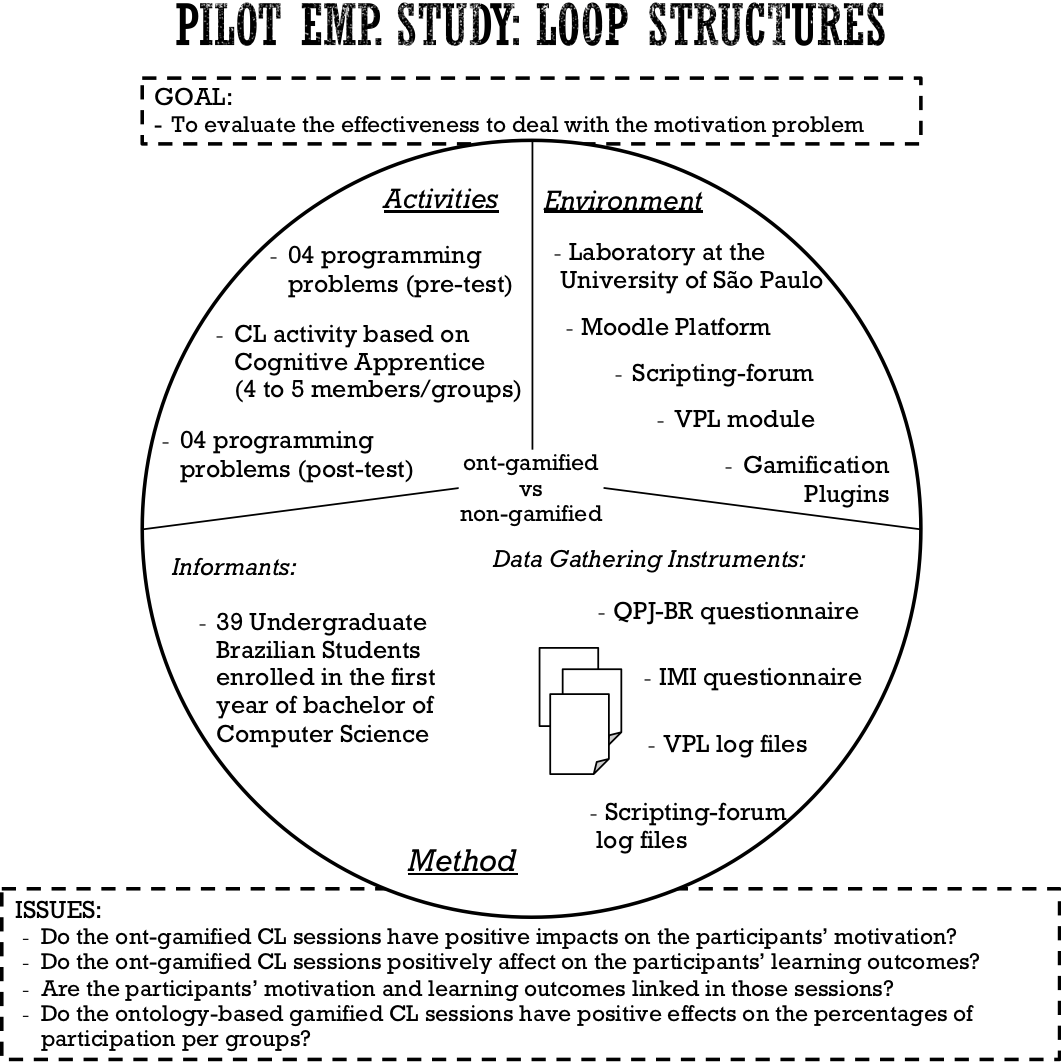
\includegraphics[width=0.63\textwidth]{images/chap-evaluation/graphical-pilot-empirical-study}\\
  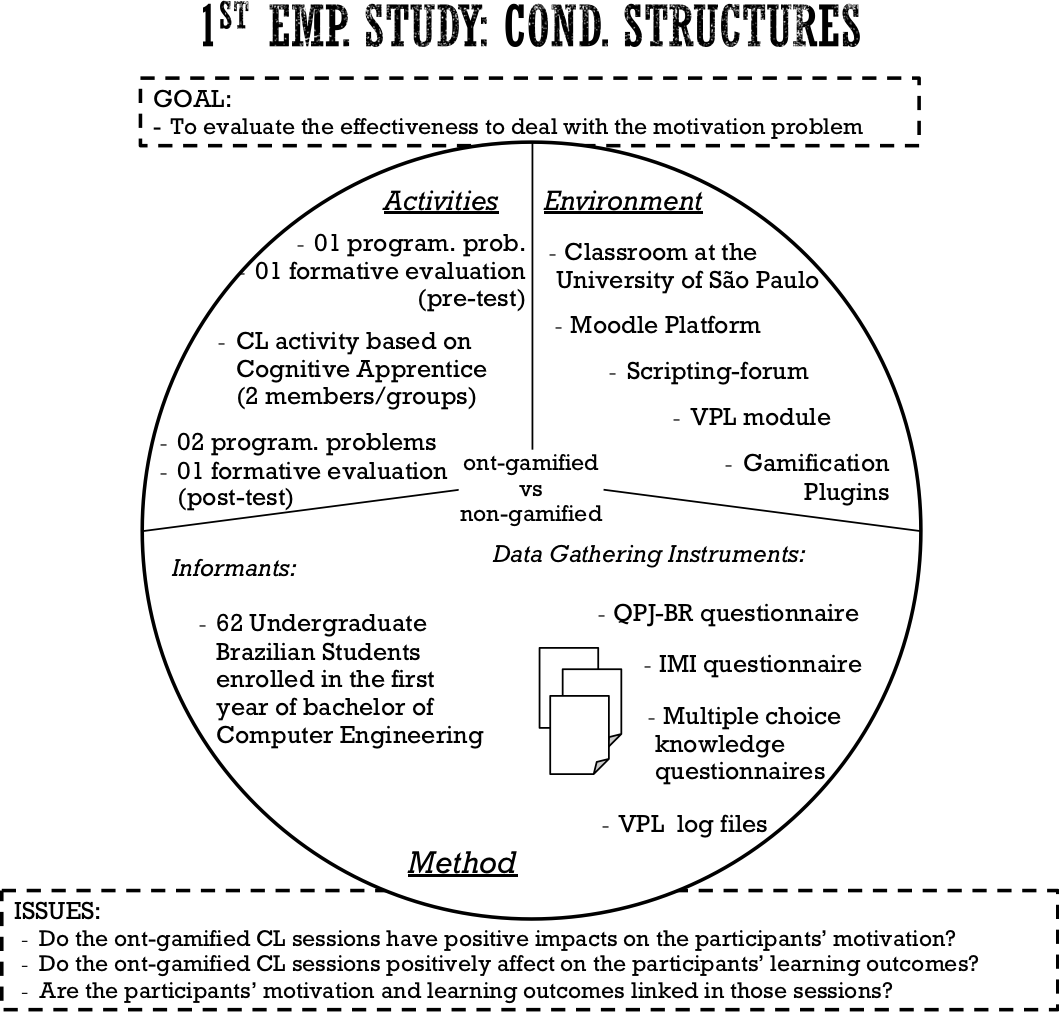
\includegraphics[width=0.63\textwidth]{images/chap-evaluation/graphical-first-empirical-study}
 \end{tabular}
 \fautor
\end{figure}

\newpage
\begin{figure}[htb]
 \caption{Graphical representation of second and third empirical studies}
 \label{fig:graphical-second-third-empirical-study}
 \centering
 \begin{tabular}{c}
  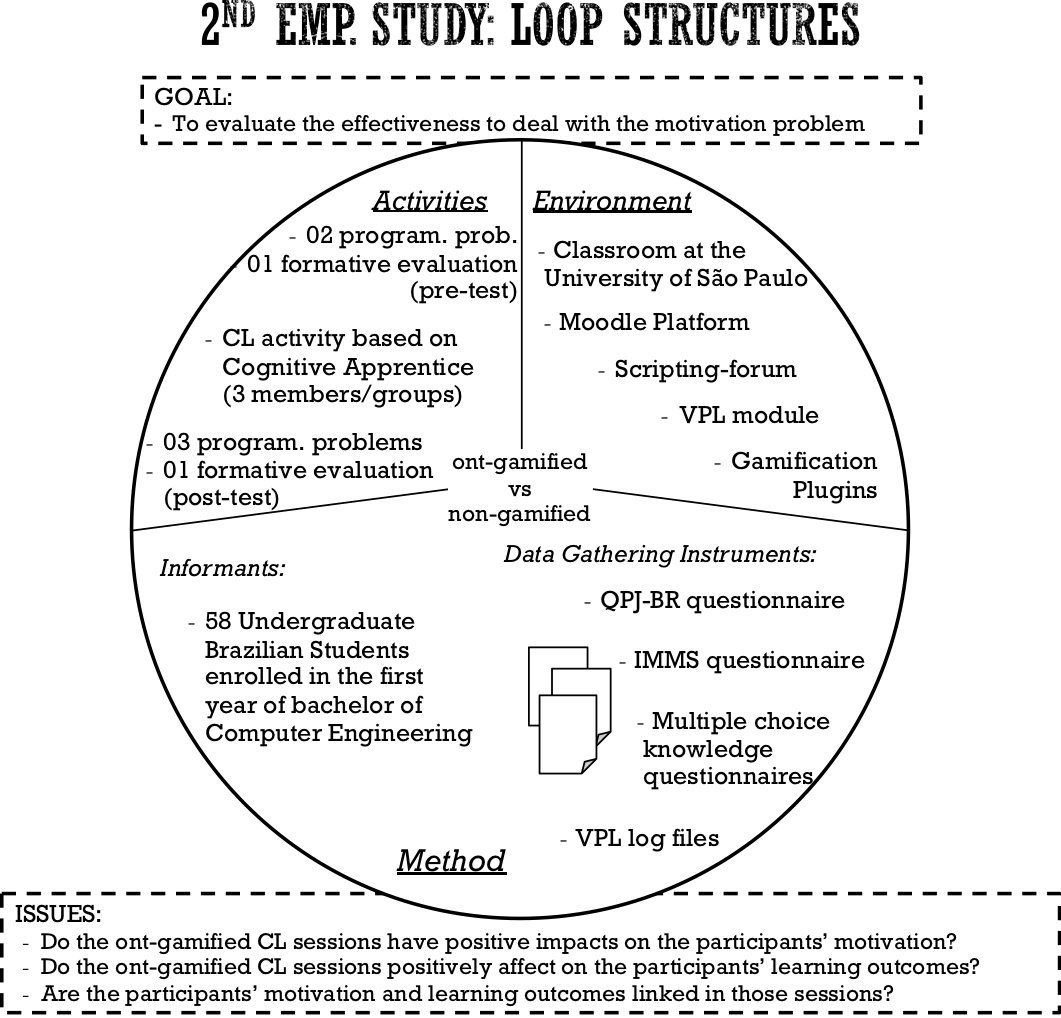
\includegraphics[width=0.63\textwidth]{images/chap-evaluation/graphical-second-empirical-study}\\
  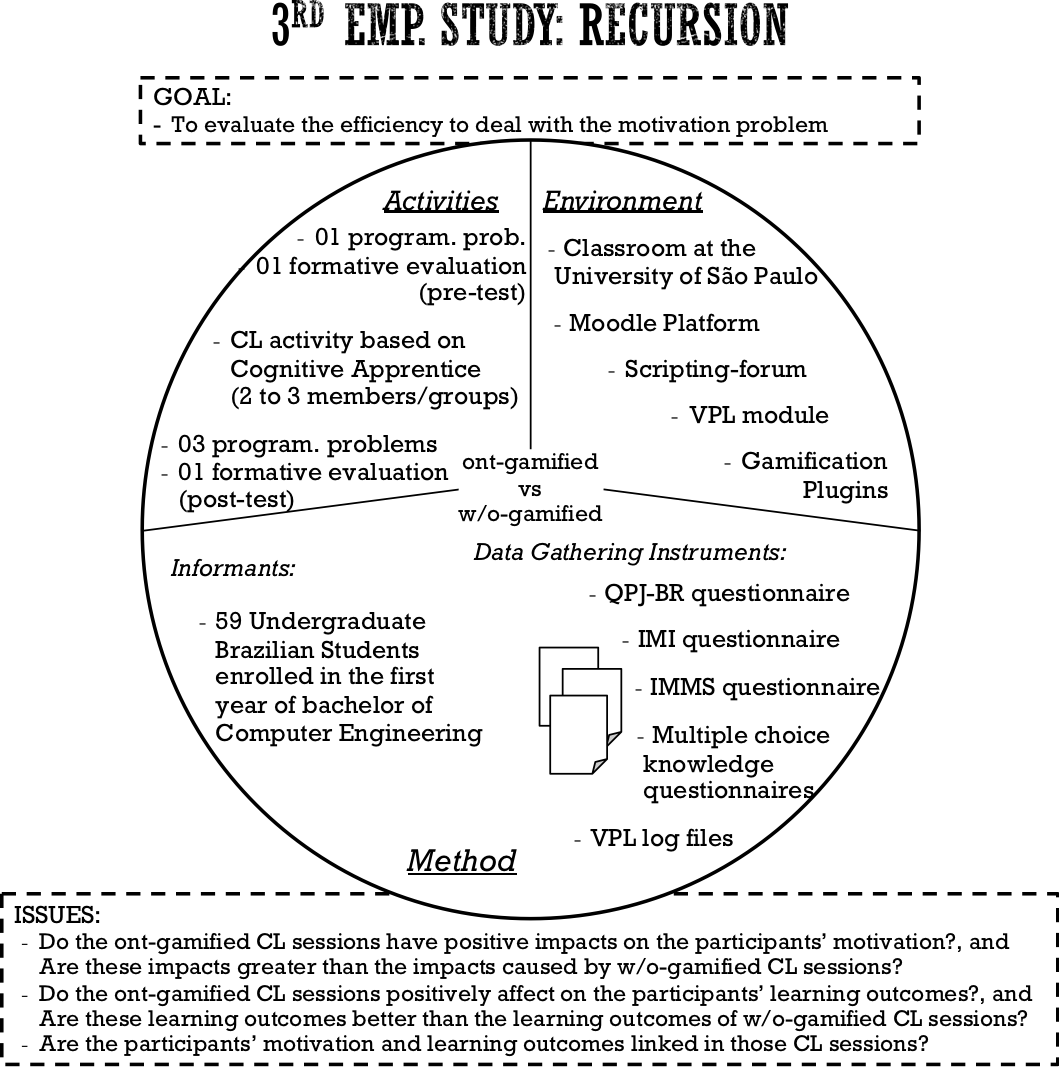
\includegraphics[width=0.63\textwidth]{images/chap-evaluation/graphical-third-empirical-study}
 \end{tabular}
 \fautor
\end{figure}

\newpage
The graphical representation for the empirical studies shown above (in \autoref{fig:graphical-pilot-first-empirical-study} and \autoref{fig:graphical-second-third-empirical-study}) is an adaptation of the Evaluand-oriented Responsive Evaluation Model (CSCL-EREM) diagram proposed by \citeonline{Jorrin-AbellanStakeMartinez-Mone2009}. The CSCL-EREM diagram, in the original version, is an artifact that summarizes the characteristics that should be taken into account by the researchers to conduct a CSCL evaluation. The diagram, employed here, is a simplified version of CSCL-EREM diagram in which only the relevant aspects of the \aspas{\emph{ontological engineering approach to gamify CL scenarios}} are summarized in the diagrams. These aspects are: the \emph{evaluand} indicated at the center of diagram; the \emph{goal} and \emph{issues} shown in dashed frames at the top and bottom of circular diagram; the educational setting features in respect to the learning \emph{environment} and \emph{activities} indicated on the left-upper and right-upper sides of the circular diagram; and the \emph{informants} and \emph{data gathering instruments} employed in the \emph{method} evaluation process shown at the bottom part of the circular diagram.

\textbf{Object of study}. The object of study is the effects of ont-gamified CL sessions on the participants' motivation and learning outcomes. The ont-gamified CL sessions have been gamified according to the suggestions given by intelligent-theory aware systems, which in turn used the ontology OntoGaCLeS as information source to give these suggestions. 
As these suggestions have been formulated employing the knowledge encoded in the ontology OntoGaCLeS to deal with the motivation problem based on well-grounded theories and practices related to gamification, the game elements were introduced in the learning environment to affect the participants' motivation, and in consequence, to produce better learning outcomes. Thus, the three issues that have been addressed in the pilot, first and second empirical studies were:

\begin{itemize}
\item Do the ontology-based gamified CL sessions have positive impacts on the participants' motivation?
\item Do the ontology-based gamified CL sessions positively affect on the participants' learning outcomes?
\item Are the participants' motivation and learning outcomes linked in those sessions?
\end{itemize}

The three issues that have been addressed in the third empirical study were:

\begin{itemize}
\item Do the ontology-based gamified CL sessions have positive impacts on the participants' motivation?, and Are these impacts better than the impacts caused by CL sessions that were gamified without the support given by the ontology OntoGaCLeS?
\item Do the ontology-based gamified CL sessions positively affect on the participants' learning outcomes?, and Are these learning outcomes better than the learning outcomes of CL sessions that were gamified without the support given by the ontology OntoGaCLeS?
\item Are the participants' motivation and learning outcomes linked in those sessions?
\end{itemize}

When the group members are adequately motivated to participate in a CL session, their levels of participation will be increased to reduce the desistance in CL activities. This effect frequently occurs and can be observed in groups with many members. In this sense, in the pilot study where the group formation for the CL sessions is defined for 4 to 5 members per groups, the issue that has been addressed in the pilot empirical study is:

\begin{itemize}
\item Do the ontology-based gamified CL sessions have positive effects on the percentage of participation per groups?
\end{itemize}

These percentages of participation per group correspond to: (1) the percentage of participants per groups having any participation that refers to a complete, semicomplete and incomplete participation level; (2) the percentage of participants per groups having an adequate participation that refers to a complete and semicomplete participation level; (3) the percentage of participants per groups having incomplete participation that refers to an incomplete and none participation level; and (4) the percentage of participants per groups without participation that refers to a none participation level. The participation levels are defined as:

\begin{itemize}
\item \emph{None participation level}: when the participant did not interact with other group members in CL sessions
\item \emph{Incomplete participation level}: when the participant interacted in CL sessions, but he/she did not complete all the necessary interactions
\item \emph{Semicomplete participation level}: when the student interacted in CL sessions performing all the necessary interactions, but he/she did not respond to all the requests made by other group members
\item \emph{Complete participation level}: when the participant interacted in CL sessions performing all the necessary interactions, and he/she responds to all the requests made by other group members
\end{itemize}
 
\textbf{Purpose}. The purpose of empirical studies was to validate the ontological engineering approach to gamify CL scenarios as a method to deal with the motivation problem caused by the scripted collaboration. 
The empirical studies were oriented to provide insights in what were the benefits of this approach in reference of the participants' motivation, and the consequence of these benefits in CL activities in which the CSCL scripts are used as method to orchestrate and structure the collaboration among the participants in the CL sessions instantiated from these scripts. Thus, in all the four empirical studies, this approach has been applied in CL activities with different levels of difficulty for their content-domains. These content-domains, from the easiest to the hardest level of difficulty, were: conditional structures, loop structures, and recursions in the course of Introduction to Computer Science. The CSCL script used to structure and orchestrate the CL sessions was a CSCL script inspired by the Cognitive Apprentice theory.

\textbf{Quality focus}. The benefits of ontology-based gamified CL sessions have been described as \emph{effectiveness} and \emph{efficiency} to deal with the motivation problem caused by the scripted collaboration. In this sense, the effectiveness was demonstrated by measuring the effects of ontology-based gamified CL sessions on the participants' motivation and learning outcomes, and then comparing the results against the results obtained from non-gamified CL sessions (\emph{ont-gamified} vs \emph{non-gamified}). Therefore, the goal in the pilot, first and second empirical studies was to evaluate the effectiveness to deal with the motivation problem; and the evaluand was ontology-based gamified and non-gamified CL sessions. The efficacy to deal with the motivation problem was defined as goal of the third empirical study, and it has been demonstrated by measuring the effects of ontology-based CL sessions on the participation' motivation and learning outcomes, and then comparing the results against the results obtained from CL sessions that were gamified without using the support given by the ontology OntoGaCLeS (\emph{ont-gamified} vs \emph{w/o-gamified}). The evaluand of this third empirical study was ontology-based gamified and CL sessions that were gamified without using the support given by the ontology OntoGaCLeS.

It is important to clarify here, that the motivation, as was explained in the \autoref{chapter:general-background}, is a construct of different factors that explains the reason whereby a human behave or act. It means that the factors to measure the participants' motivation vary according to the chosen theory to explain certain behavior or actions, the context in which the theory is applied, and the interest under study in each theory. In the empirical studies, to validate the ontological engineering approach to gamify CL scenarios, two theories were used to measure the participants' motivation. These two theories were: the SDT theory and the ARCS model of motivation.

\begin{itemize}
\item
In the SDT theory \cite{RyanDeci2000}, the construct of motivation is defined as the degree of an individual owns to behave or act based on factors related to the self-determination and self-regulation. In this sense, the construct of motivation is known as intrinsic motivation, and the instrument used to measure it in the empirical studies was an adapted Portuguese version of the Intrinsic Motivation Inventory (IMI), where the factors to measure the intrinsic motivation are: the interest/enjoyment, perceived choice, felt of pressure/tension, effort/importance, perceived competence, value/usefulness and relatedness.

\item
In the ARCS model \cite{Keller2009}, the construct of motivation is based on the expectancy-value theory in which is assumed that an individual is motivated if he/she sees value in his/her acts or behaviors and if there is an optimistic expectation for success in this acts or behaviors \cite{Wigfield1994}. Hence, the factors related to the construct of motivation in the model ARCS are: attention, relevance, confidence and satisfaction.
\end{itemize}

It is important highlight here, that, to measure the intrinsic motivation using the IMI instrument, usually, not all factors are necessary. The interest/enjoyment is only considered per se the self-report measure of intrinsic motivation. The perceived choice and perceived competence are positive predictors, the pressure/tension is the negative predictor, the value/usefulness and effort/importance are factors related to the internalization of motivation, and the relatedness factor is only applicable in context of interpersonal and friendship activities. Therefore, in the pilot, first and third empirical studies the adapted Portuguese version of the IMI questionnaire has been used as data gathering instrument to measure: the \emph{interest/enjoyment} as the factor directly related to measure the intrinsic motivation, the \emph{perceived choice} as the only positive predictor, the \emph{pressure/tension} as the negative predictor, and the \emph{effort/importance} as the only factor related with the internalization of motivation.

The data gathering instrument used to measure the motivation as factors based on the ARCS model in the second and third empirical studies was the adapter Portuguese version of Instructional Materials Motivation Survey (IMMS) questionnaire. The measurement given by this instrument was the \aspas{\emph{level of motivation}} that consists in the factors: \emph{attention}, \emph{relevance} and \emph{satisfaction}. The confidence factor has been removed from the original ARCS model to avoid an overlapping of factors with the IMI questionnaire because the confidence and perceived choice are factors related to the self-regulation. Thus, the \emph{level of motivation} is a constructor defined to refer the motivation that is completely separated from the intrinsic motivation.

\textbf{Perspective}. The perspective for the empirical studies came from the viewpoint of the instructional designers and researchers.

\begin{itemize}
\item
Instructional designers would like to know the benefits of using ontology-based gamification CL sessions instead to use non-gamified CL session or CL sessions that are gamified without using the support given by the ontology OntoGaCLeS. In this sense, the pilot study and the first two full-scale studies presented here compare the effects of ontology-based gamified CL sessions (\emph{ont-gamified}) and non-gamified CL scenarios (\emph{non-gamified}), whereas the third full-scale study compares the effects of ontology-based gamified CL sessions (\emph{ont-gamified}) and CL sessions that were gamified without using the support given by the ontology OntoGaCLeS (\emph{w/o-gamified}).

\item
Researchers would like to know if the ontological engineering approach to gamify CL scenarios, as a method proposed in this dissertation, is effective and efficient method to deal with the motivation problem caused by the scripted collaboration. 
\end{itemize}

\textbf{Context}. The context in which the empirical studies has been conducted were the CL activities in which the CL sessions have been instantiated from a CSCL script inspired by an instructional/learning theory. 
Particularly, in the empirical studies conducted to validate the ontological engineering approach to gamify the CL scenarios, the CSCL script used to design and to orchestrate the interaction among the participants was a CSCL script inspired by the Cognitive Apprentice theory, and the domain-contents for which the scripts have been instantiated as CL sessions were three subjects related to the course of \aspas{Introduction to Computer Science.} Thus, different difficulty levels of subjects were employed in the instantiation of the CL sessions in the empirical studies, these subjects from the easiest difficulty level to the most difficult level were: the subject of conditional structures for the first empirical study, the subject of loop structures for the pilot and second empirical study, and the subject of recursion for the third empirical study.

%% ========================== %%

\subsection{Hypothesis Formulation}

In order \emph{to evaluate the effectiveness to deal with the motivation problem} caused by the scripted collaboration (First Goal, \emph{g1}), the first issue addressed in the pilot and first empirical studies was \aspas{\emph{Do the ontology-based gamified CL sessions have positive impacts on the participants' motivation}?} by testing the:

\begin{description}
\item[Null hypothesis, $H_{null,IM,g1}$:] \aspas{\emph{There was no significant difference between the intrinsic motivation of students who participated in ontology-based gamified CL sessions and the intrinsic motivation of students who participated in non-gamified CL sessions},} against the
\item[Alternative hypothesis, $H_{alt,IM,g1}$:] \aspas{\emph{The intrinsic motivation of students who participated in ontology-based gamified CL sessions was greater than the intrinsic motivation of students who participated in non-gamified CL sessions}.}
\end{description}

In the second empirical study, this first issue was addressed by testing the:  

\begin{description}
\item[Null hypothesis, $H_{null,LoM,g1}$:] \aspas{\emph{There was no significant difference between the level of motivation obtained by students who participated in ontology-based gamified CL sessions and the level of motivation obtained by students who participated in non-gamified CL sessions},} against the
\item[Alternative hypothesis, $H_{alt,LoM,g1}$:] \aspas{\emph{The level of motivation obtained by students who participated in ontology-based gamified CL sessions was greater than the level of motivation obtained by students who participated in non-gamified CL sessions}.}
\end{description}

The second issue \aspas{\emph{Do the ontology-based gamified CL sessions positively affect on the participants' learning outcomes}?} has been addressed in the pilot, first and second empirical studies by testing the:

\begin{description}
\item[Null hypothesis, $H_{null,GSK,g1}$:] \aspas{\emph{There was no significant difference between the gains in skill/knowledge obtained by students who participated in ontology-based gamified CL sessions and the gains in skill/knowledge obtained by students who participated in non-gamified CL sessions},} against the
\item[Alternative hypothesis, $H_{alt,GSK,g1}$:] \aspas{\emph{The gains in skill/knowledge obtained by students who participated in ontology-based gamified CL sessions was greater than the gains in skill/knowledge obtained by students who participated in non-gamified CL sessions}.}
\end{description}

In the pilot, first, and second empirical studies, the third issue \aspas{\emph{Are the participants' motivation and learning outcomes linked in either the non-gamified CL sessions or the ontology-based gamified CL sessions}?} has been addressed by testing the:

\begin{description}
\item[Null hypothesis, $H_{null,\rho,g1}$:] \aspas{\emph{There was no significant correlation between the participants' motivation and their gains in skill/knowledge in either the non-gamified CL sessions or the ontology-based gamified CL sessions},} against the
\item[Alternative hypothesis, $H_{alt,\rho,g1}$:] \aspas{\emph{There was a significant correlation between the participants' motivation and their gains in skill/knowledge in either the non-gamified CL sessions or the ontology-based gamified CL sessions}.}
\end{description}

The four issue \aspas{\emph{Do the ontology-based gamified CL sessions have positive effects on the percentages of participation per groups}?} has been addressed in the pilot empirical study by testing the:

\begin{description}
\item[Null hypothesis, $H_{null,Pct,g1}$:] \aspas{\emph{
There was no significant difference between the percentages of participation per groups in ontology-based gamified CL sessions and the percentages of participation per groups in non-gamified CL sessions},} against the
\item[Alternative hypothesis, $H_{alt,Pct,g1}$:] \aspas{\emph{
The percentages of participation per groups in ontology-based gamified CL sessions are better than the percentage of participation per groups in non-gamified CL sessions}.}
\end{description}

In order \emph{to evaluate the efficiency to deal with the motivation problem} caused by the scripted collaboration (Second Goal, \emph{g2}), the first issue  \aspas{\emph{
Do the ontology-based gamified CL sessions have positive impacts on the participants' motivation?, and Are these impacts better than the impacts caused by CL sessions that were gamified without the support given by the ontology OntoGaCLeS
}?}
has been addressed in the third empirical study by testing the:

\begin{description}
\item[Null hypothesis, $H_{null,IM,g2}$:] \aspas{\emph{There was no significant difference between the intrinsic motivation of students who participated in ontology-based gamified CL sessions and the intrinsic motivation of students who participated in CL sessions that were gamified without the support given by the ontology OntoGaCLeS},} against the
\item[Alternative hypothesis, $H_{alt,IM,g2}$:] \aspas{\emph{The intrinsic motivation of students who participated in ontology-based gamified CL sessions was greater than the intrinsic motivation of students who participated in CL sessions that were gamified without the support given by the ontology OntoGaCLeS}.}
\end{description}

\begin{description}
\item[Null hypothesis, $H_{null,LoM,g2}$:] \aspas{\emph{There was no significant difference between the level of motivation obtained by students who participated in ontology-based gamified CL sessions and the level of motivation obtained by students who participated in CL sessions that were gamified without the support given by the ontology OntoGaCLeS},} against the
\item[Alternative hypothesis, $H_{alt,LoM,g2}$:] \aspas{\emph{The level of motivation obtained by students who participated in ontology-based gamified CL sessions was greater than the level of motivation obtained by students who participated in CL sessions that were gamified without the support given by the ontology OntoGaCLeS}.}
\end{description}

In the third empirical study, the second issue \aspas{\emph{
Do the ontology-based gamified CL sessions positively affect on the participants' learning outcomes?, and Are these learning outcomes better than the learning outcomes of CL sessions that were gamified without the support given by the ontology OntoGaCLeS}?} has been addressed by testing the:

\begin{description}
\item[Null hypothesis, $H_{null,GSK,g2}$:] \aspas{\emph{There was no significant difference between the gains in skill/knowledge obtained by students who participated in ontology-based gamified CL sessions and the gains in skill/knowledge obtained by students who participated in CL sessions that were gamified without the support given by the ontology OntoGaCLeS},} against the
\item[Alternative hypothesis, $H_{alt,GSK,g2}$:] \aspas{\emph{The gains in skill/knowledge obtained by students who participated in ontology-based gamified CL sessions was greater than the gains in skill/knowledge obtained by students who participated in CL sessions that were gamified without the support given by the ontology OntoGaCLeS}.}
\end{description}

The third issue \aspas{\emph{Are the participants' motivation and learning outcomes linked in either the ontology-based gamified CL sessions and the CL sessions that were gamified without using the support given by the ontology OntoGaCLeS}?} has been addressed in the third empirical study by testing the:

\begin{description}
\item[Null hypothesis, $H_{null,\rho,g2}$:] \aspas{\emph{There was no significant correlation between the participants' motivation and their gains in skill/knowledge in either the ontology-based gamified CL sessions or the CL sessions that were gamified without using the support given by the ontology OntoGaCLeS},} against the
\item[Alternative hypothesis, $H_{alt,\rho,g2}$:] \aspas{\emph{There was a significant correlation between the participants' motivation and their gains in skill/knowledge in either the ontology-based gamified CL sessions or the CL sessions that were gamified without using the support given by the ontology OntoGaCLeS}.}
\end{description}

%% ========================== %%

\subsection{Variables Selection}

\autoref{tab:variables-empirical-studies} summarizes the variables involved in the empirical studies with the type of values for the variables and a brief explanation of them. The independent variables \aspas{\emph{Type}} determined the type of CL sessions for which the evaluation of the ontological engineering approach to gamify CL scenario were carried out. Thus, when the goal of the empirical study was to evaluate the effectiveness of dealing with the motivation problem ($g1$), the types of CL sessions were: ontology-based gamified CL sessions and non-gamified CL sessions; and when the goal of the empirical study was to evaluate the efficiency of dealing with the motivation problem ($g2$), the types of CL sessions were: ontology-based gamified CL sessions (\emph{ont-gamified}) and CL sessions that were gamified without using the support given by the ontology OntoGaCLeS (\emph{w/o-gamified}).

\setlongtables{\small
\begin{longtable}{cllc}\caption{Independent and dependent variables for the empirical studies} \tabularnewline
\hline\hline
\multicolumn{1}{c}{Name}&\multicolumn{1}{c}{Values}&\multicolumn{1}{c}{Description}&\multicolumn{1}{c}{Studies}\tabularnewline
\hline
\endfirsthead\caption[]{\em (continued)} \tabularnewline
\hline
\multicolumn{1}{c}{Name}&\multicolumn{1}{c}{Values}&\multicolumn{1}{c}{Description}&\multicolumn{1}{c}{Studies}\tabularnewline
\hline
\endhead
\hline
\endfoot
\label{tab:variables-empirical-studies}
%\multicolumn{4}{l}{\emph{Dependent Variables}:}\tabularnewline \hline
Type &
\multicolumn{1}{p{2.5cm}}{\{\emph{ont-gamified}, \emph{non-gamified}\}} &
\multicolumn{1}{p{8.5cm}}{To evaluate the effectiveness, each student participated in one of these two types of CL scenarios during the empirical studies} &
\multicolumn{1}{p{1.5cm}}{\centering pilot, first, second}
\tabularnewline \hline

Type &
\multicolumn{1}{p{2.5cm}}{\{\emph{ont-gamified}, \emph{w/o-gamified}\}} &
\multicolumn{1}{p{8.5cm}}{To evaluate the efficiency, each student participated in one of these two types of CL scenarios during the empirical studies} &
\multicolumn{1}{p{1.5cm}}{\centering third}
\tabularnewline \hline

\multicolumn{4}{l}{\emph{Controller Variables}:}\tabularnewline \hline

CLRole &
\multicolumn{1}{p{2.5cm}}{\{\mbox{\emph{Master}}, \mbox{\emph{Apprentice}\}}} &
\multicolumn{1}{p{8.5cm}}{The CL role played by each participant in the CL sessions instantiated from a CSCL script inspired by the Cognitive Apprenticeship theory.
These roles are assigned for a participant according to his/her current knowledge/skill state} &
\multicolumn{1}{p{1.5cm}}{\centering pilot, first, second, third}
\tabularnewline \hline

\multicolumn{4}{l}{\emph{Dependent Variables}:}\tabularnewline \hline

\multicolumn{1}{p{2cm}}{\centering \mbox{Intrinsic} \mbox{Motivation}} &
\multicolumn{1}{p{2.5cm}}{\centering \emph{logits}} &
\multicolumn{1}{p{8.5cm}}{The intrinsic motivation estimates for the participants as the factors: interest/enjoyment, perceived choice, pressure/tension, and effort/importance. This dependent variable and its factors have been measured on a \emph{logit} scale} &
\multicolumn{1}{p{1.5cm}}{\centering pilot, first, third}
\tabularnewline \hline

\multicolumn{1}{p{2cm}}{\centering \mbox{Level} of \mbox{Motivation}} &
\multicolumn{1}{p{2.5cm}}{\centering \emph{logits}} &
\multicolumn{1}{p{8.5cm}}{The level of motivation estimates for the participants as the factors: attention, relevance, and satisfaction. This dependent variable and its factors have been measured on a \emph{logit} scale} &
\multicolumn{1}{p{1.5cm}}{\centering second, third}
\tabularnewline \hline

\multicolumn{1}{p{2cm}}{\centering \mbox{Gains} in \mbox{Skill}/\mbox{Knowledge}} &
\multicolumn{1}{p{2.5cm}}{\centering \emph{logits}} &
\multicolumn{1}{p{8.5cm}}{The gains in skill/knowledge for the participants were measured as learning outcomes employing irt-models for programming problems and multiple choice knowledge questionnaires on a \emph{logit} scale} &
\multicolumn{1}{p{1.5cm}}{\centering pilot, first, second, third}
\tabularnewline \hline


\multicolumn{1}{p{2cm}}{\centering Pct. of \mbox{Participation} per \mbox{Groups}} &
\multicolumn{1}{p{2.5cm}}{\centering \mbox{\emph{Pct.}}} &
\multicolumn{1}{p{8.5cm}}{The percentages of participation per group. These percentages correspond to the 
pct. of students without participation, pct. of students having participation, pct. of students having incomplete participation, and pct. of students having adequate participation.} &
\multicolumn{1}{p{1.5cm}}{\centering pilot}
\tabularnewline \hline

\end{longtable}}

%% ========================== %%

\subsection{Selection of Subjects}

According to the real situation in which the empirical studies were carried out, the subjects for the empirical studies were chosen based on convenience. The subjects were students signed-up in the course of Introduction to Computer Science taught by the Prof. Seiji Isotani to the graduate programs in Computer Science and Computer Engineering at the University of São Paulo during the second semester of 2016 (August -  December) and the first semester of 2017 (March - July). Thus, the selection of subjects, described as informants in the CSCL-EREM diagrams of \autoref{fig:graphical-pilot-first-empirical-study} and \autoref{fig:graphical-second-third-empirical-study} for each empirical study, were: 

\begin{description}
\item[For the pilot empirical study,]
39 undergraduate Brazilian students enrolled in the first year of bachelor of Computer Science at the University of São Paulo.
\item[For the first empirical study,]
62 undergraduate Brazilian students enrolled in the first year of bachelor of Computer Engineering at the University of São Paulo.
\item[For the second empirical study,]
58 undergraduate Brazilian students enrolled in the first year of bachelor of Computer Engineering at the University of São Paulo.
\item[For the third empirical study,]
59 undergraduate Brazilian students enrolled in the first year of bachelor of Computer Engineering at the University of São Paulo.
\end{description}

The participants in the empirical studies were chosen from a homogeneous population in the age range from 17 to 25 years old, sharing the same social-economy status and culture. 

%% ========================== %%
\subsection{Design}

Employing the scoping, hypothesis formulation, variables selection, and selection of subjects detailed in the previous subsections, the principles to design the four empirical studies were:

\begin{description}
\item[Randomization.] The CL role was not randomly assigned to the students in the empirical studies. If the student known how to use the cognitive or meta-cognitive skill and had experience in how to use this skill, he/she played the master role, otherwise the student played the apprentice role. The students as subjects of empirical studies were not selected randomly, they were the students signed-up to the course of Introduction to Computer Science at the University of São Paulo during the second semester of 2016 and the first semester of 2017. With these students as subjects of empirical studies, a theory-driven group formation was carried out according to the pseudo-algorithm proposed by \citeonline{IsotaniMizoguchi2008a}; and then, randomly, one half of the groups were assigned to participate in one of two types of CL sessions defined as \emph{evaluand} in each empirical study, whereas the other half of groups was assigned to participate in the other type of CL sessions. Thus, for the pilot, first and second empirical studies, one half of groups defined by the theory-driven group formation was randomly chosen to participate in non-gamified CL sessions, and the other half of groups was chosen to participate in ontology-based CL sessions.
For the third empirical study, one half of groups was randomly participated in ontology-based CL sessions, and the other half of groups participated in CL session that were gamified without using the support given by the ontology OntoGaCLeS.

\item[Blocking.] No systematic approach to block the independent and controlled variable has been applied in the empirical studies. The decision to assign CL roles for the students as subject of empirical studies was based on their current skill/knowledge states, so that this decision could be considered a way to block the impact of students having different levels of knowledge and having different levels of cognitive or meta-cognitive skills. 
 
\item[Balancing.] The empirical studies did not have a balanced design because they were conducted in real situations, the course of Introduction to Computer Science at the University of São Paulo during the 2nd semester of 2016 and the 1st semester of 2017.
\end{description}

According to the principles mentioned above, the four empirical studies have been defined as quasi-experiments with a $2\times2$ factorial design, and with a randomized assignment of the type of CL session for the groups defined by the theory-driven group formation proposed by \citeonline{IsotaniMizoguchi2008a}. Furthermore, each empirical study has been conducted in three phases: pre-test phase, intervention phase, and post-test phase. During the pre-test phase, the skill and knowledge levels of students were estimated to assign the CL roles. The necessary and desired conditions to assign Player roles for the participants have also been obtained in the pre-test phase through a questionnaire of player types. The gains in skill/knowledge for the participants were estimated as the difference of their skill and knowledge obtained in the post-test phase and their skill and knowledge obtained in the pre-test phase. In the post-test phase, motivation surveys were applied to the participants for measuring the participants' motivation as measurement of the intrinsic motivation and the level of motivation.

%% ========================== %%
\subsection{Instrumentation}
\label{subsec:instrumentation}

As was shown in the conceptual flow to gamify CL sessions using the knowledge described in the ontology OntoGaCLeS (\autoref{fig:conceptual-flow-gamify-cl-sessions}), to obtain the ontology-based gamified CL sessions, it is necessary to have the information about the necessary and desired conditions to assign player roles for the subjects (students) in each empirical study. This information has been collected in the Moodle platform through a Web-based version of QPJ-BR questionnaire \cite{AndradeMarquesBittencourtIsotani2016}. This questionnaire is detailed in \autoref{annex:QPJ-BR-questionnaire}.

Programming problem tasks and multiple choice knowledge questionnaires were used as information sources to estimate the skill and knowledge of participants in the pre-test and post-test phases. The skill and knowledge estimates from pre-test was also be used to assign the CL roles for the participants of empirical studies.
\autoref{tab:programming-problem-multiple-choice-questionnaires} shows the programming problem tasks and multiple choice knowledge questionnaires employed in the empirical studies.
All of the programming problem tasks were implemented in an adapted version of \emph{VPL module}\footnote{Virtual Programming Lab for Moodle 2 with screen and code recordings - \url{https://github.com/geiser/moodle-mod_vpl}}, and the multiple choice knowledge questionnaires were developed using the \emph{AMC software}\footnote{Software to create multiple choice questionnaires - \url{https://www.auto-multiple-choice.net/}}

\setlongtables{\small
\begin{longtable}{cccp{9cm}c}\caption{Programming problem tasks and multiple choice knowledge questionnaires} \tabularnewline
\hline\hline
\multicolumn{1}{c}{Code}&\multicolumn{1}{c}{Study}&\multicolumn{1}{c}{Phase}&\multicolumn{1}{c}{Title}&\multicolumn{1}{c}{\autoref{annex:data-gathering-instruments-skill-knowledge}}\tabularnewline
\hline
\endfirsthead\caption[]{\em (continued)} \tabularnewline
\hline
\multicolumn{1}{c}{Code}&\multicolumn{1}{c}{Study}&\multicolumn{1}{c}{Phase}&\multicolumn{1}{c}{Title}&\multicolumn{1}{c}{\autoref{annex:data-gathering-instruments-skill-knowledge}}\tabularnewline
\hline
\endhead
\hline
%\multicolumn{6}{r}{\tiny Signif. codes:  0 \aspas{**} 0.01 \aspas{*} 0.05}
\endfoot
\label{tab:programming-problem-multiple-choice-questionnaires}

P1'&pilot&pre-test&
Programming Problem: Calculate the proper divisors of a number (\emph{Divisores próprios})
&\autoref{annex:pilot-study-p1} \tabularnewline

P2'&pilot&pre-test&
Programming Problem: Calculate the sum of prime divisors of number (\emph{Soma dos divisores próprios})
&\autoref{annex:pilot-study-p2} \tabularnewline

P3'&pilot&pre-test&
Programming Problem: Calculate distance of rebounds for an elastic ball (\emph{Distância dos rebates da bola de elástico})
&\autoref{annex:pilot-study-p3} \tabularnewline

P4'&pilot&pre-test&
Programming Problem: Calculate the maximum length of a hailstone sequence (\emph{Máximo comprimento das sequências de números granizo})&
\autoref{annex:pilot-study-p4} \tabularnewline

PA'&pilot&post-test&
Programming Problem: Calculate the Inverse Fibonacci sequence on base $n$ and $m$ (\emph{Sequência inversa Fibonacci de base $n$ e $m$})&
\autoref{annex:pilot-study-pA} \tabularnewline

PB'&pilot&post-test&
Programming Problem: Calculate the absolute difference between odd and even numbers in an inverse Fibonacci sequence (\emph{Diferença absoluta entre os números pares e ímpares na sequência inversa Fibonacci})&
\autoref{annex:pilot-study-pB} \tabularnewline

PC'&pilot&post-test&
Programming Problem: Calculate the i-th prize of a machine slot (\emph{O i-ésimo prêmio da caça-níquel)})&
\autoref{annex:pilot-study-pC} \tabularnewline

PD'&pilot&post-test&
Programming Problem: Calculate the highest prize of a machine slot (\emph{Ganhando o prêmio maior da caça-níquel})&
\autoref{annex:pilot-study-pD} \tabularnewline

P1&first&pre-test&
Programming Problem: Develop a simple virtual temperature monitor(\emph{Monitor de Temperatura Virtual})&
\autoref{annex:first-study-p1}\tabularnewline

p1a&first&pre-test&
Formative Evaluation: Multiple choice knowledge questionnaires of cond. structures (\emph{provinha1a})&
\autoref{annex:first-study-pre}\tabularnewline


PA&first&post-test&
Programming Problem: Develop a Basal Metabolic Rate (\emph{TMB - Taxa Metabólica Basal})&
\autoref{annex:first-study-pA}\tabularnewline

PB&first&post-test&
Programming Problem: Develop a diet calculator (\emph{Calculadora de dieta})&
\autoref{annex:first-study-pB}\tabularnewline

p1b&first&pre-test&
Formative Evaluation: Multiple choice knowledge questionnaires of cond. structures (\emph{provinha1b})&
\autoref{annex:first-study-pos}\tabularnewline

P2&second&pre-test&
Programming Problem: Calculate the proper divisors of a number (\emph{Divisores próprios})&
\autoref{annex:second-study-p2}\tabularnewline

P3&second&pre-test&
Programming Problem: Calculate the maximum length of a hailstone sequence (\emph{Máximo comprimento das sequências de números granizo})&
\autoref{annex:second-study-p3}\tabularnewline

p2a&second&pre-test&
Formative Evaluation: Multiple choice knowledge questionnaires of loop structures (\emph{provinha2a})&
\autoref{annex:second-study-pre}\tabularnewline

PC&second&post-test&
Programming Problem: Calculate a geometric sequence (\emph{Sequências de potências})&
\autoref{annex:second-study-pC}\tabularnewline

PD&second&post-test&
Programming Problem: Calculate global minimum coin changes (\emph{Caixa eletrônico})&
\autoref{annex:second-study-pD}\tabularnewline

PE&second&post-test&
Programming Problem: Count number of semi-primes for RSA (\emph{Contagem de semi-primos para o algoritmo RSA})&
\autoref{annex:second-study-pE}\tabularnewline

p2b&second&post-test&
Formative Evaluation: Multiple choice knowledge questionnaires of loop structures (\emph{provinha2b})&
\autoref{annex:second-study-pos}\tabularnewline

P4&third&pre-test&
Programming Problem: Calculate fibonacci polynomials (\emph{Polinômios de Fibonacci})&
\autoref{annex:third-study-p4}\tabularnewline

p3a&third&pre-test&
Formative Evaluation: Multiple choice knowledge questionnaires of recursion (\emph{provinha3a})&
\autoref{annex:third-study-pre}\tabularnewline

PF&third&post-test&
Programming Problem: Generation of planning poker sequence (\emph{Planning Poker})&
\autoref{annex:third-study-pF}\tabularnewline

PG&third&post-test&
Programming Problem: Counting palindromes (\emph{Contagem de palindromos})&
\autoref{annex:third-study-pG}\tabularnewline

PH&third&post-test&
Programming Problem: Maze solving algorithm (\emph{A saída do labirinto})&
\autoref{annex:third-study-pH}\tabularnewline

p3c&third&post-test&
Formative Evaluation: Multiple choice knowledge questionnaires of recursion (\emph{provinha3c})&
\autoref{annex:third-study-pos}\tabularnewline

\hline
\end{longtable}}

In the empirical studies, the data gathering instruments used to measure the participants' motivation were:
\begin{itemize}
\item
a Web-based questionnaire for the adapted Portuguese version of the Intrinsic Motivation Inventory (\autoref{annex:data-gathering-instruments-motivation}: \autoref{annex:IMI-pilot-study}) employed in the pilot empirical study to gather information related to the participants' intrinsic motivation
\item
a Paper-based questionnaire for the adapted Portuguese version of the Intrinsic Motivation Inventory (\autoref{annex:data-gathering-instruments-motivation}: \autoref{annex:IMI-first-study}) employed in the first empirical study to gather information related to the participants' intrinsic motivation
\item
a Paper-based questionnaire for the adapted Portuguese version of the Instructional Materials Motivation Survey (\autoref{annex:data-gathering-instruments-motivation}: \autoref{annex:IMMS-second-study}) employed in the second empirical study to gather information related to the participants' level of motivation
\item
a Web-based questionnaire for the adapted Portuguese version of the Intrinsic Motivation Inventory and the adapted Portuguese Instructional Materials Motivation Survey (\autoref{annex:data-gathering-instruments-motivation}: \autoref{annex:IMI-IMMS-third-study}) employed in the third empirical study to gather information related to the participants' intrinsic motivation and level of motivation
\end{itemize}

The ontology-based gamified CL sessions in the empirical studies were obtained through the conceptual flow to gamify CL sessions shown in \autoref{fig:conceptual-flow-gamify-cl-sessions}, so that the information encoded in the \aspas{\emph{ontological model to apply gamification as persuasive technology in CL scenarios based on the Cognitive Apprenticeship theory and with the player roles based on the Yee's model to personalize the gamification}} has been used with the \emph{Gamification plugins} in the Moodle platform to define the ontology-based gamified CL sessions. However, due to the lack of automatic support given by the Gamification plugins to set and to configure the game elements in the Moodle learning environment, the gamified CL sessions were not obtained using all the three ontological structures to represent gamified CL scenarios described in this model. In this sense, only two of three ontological structures to represent gamified CL scenarios were employed at the same time in each empirical study to set and configure the Gamification plugins, Thus,

\begin{itemize}
\item For the pilot, first and second empirical studies, the ontological structures to represent \aspas{\emph{Gamified Cognitive Apprenticeship Scenario for Master/Yee Achiever and Apprentice/Yee Achiever}} and \aspas{\emph{Gamified Cognitive Apprenticeship Scenario for Master/Yee Socializer and Apprentice/Yee Socializer}} were used to obtain the ontology-based gamified CL sessions.
\item For the third empirical study, the ontological structures to represent \aspas{\emph{Gamified Cognitive Apprenticeship Scenario for Master/Yee Achiever and Apprentice/Yee Achiever}} and \aspas{\emph{Gamified Cognitive Apprenticeship Scenario for Master/Social Achiever and Apprentice/Social Achiever}} were used to obtain the ontology-based gamified CL sessions.%detail in appendix the screens and CSCL script-
\end{itemize}

Finally, in all the types of CL sessions (ont-gamified CL sessions, non-gamified CL sessions, and w/o-gamified CL sessions), a CSCL script inspired by the Cognitive Apprenticeship theory and illustrated in \autoref{fig:cognitive-apprenticeship-cscl-script} was used as a method to orchestrate and structure the collaboration among the participants. This script was implemented as an activity in the Moodle platform by employing the \emph{Scripting-forum module}\footnote{Available at the URL: \url{https://github.com/geiser/moodle\_scripting\_forum}}.

%\subsubsection*{non-gamified CL sessions}
%\subsubsection*{w/o-gamified CL sessions}
%The CL sessions that were gamified without using the support given by the ontology OntoGaCLeS.
%\subsubsection*{Ontology-based gamified CL sessions}
%The independent variables \aspas{\emph{Type}} determined the type of CL sessions for which the evaluation of the ontological engineering approach to gamify CL scenario were carried out. Thus, when the goal of the empirical study was to evaluate the effectiveness of dealing with the motivation problem, the types of CL sessions were: ontology-based gamified CL sessions and non-gamified CL sessions; and when the goal of the empirical study was to evaluate the efficiency of dealing with the motivation problem, the types of CL sessions were: ontology-based gamified CL sessions (\emph{ont-gamified} CL sessions) and CL sessions that have been gamified without using the support given by the ontology OntoGaCLeS (\emph{w/o-gamified} CL sessions).

%% ========================== %%
\subsection{Schedule, Timing, and Data Collection Procedure}
\label{subsec:data-collection-procedure}

\textbf{Preparation:} The aspects under study in the empirical studies and the hypotheses stated in this dissertation were not informed to the participants (students) of the empirical studies, but they were aware that the researcher wanted to use the data gathered by their participation in the course. All participants (students) were guaranteed anonymity, and all materials that were used in the data collection procedure were prepared in advance. Previously to the intervention phase, as part of the preparation phase, the students were instructed in how to participate in the CL activity using the \emph{Scripting-forum module} in the Moodle platform.

\subsubsection{Execution: Pilot Empirical Study}

The pilot empirical study was executed over three weeks with the schedule, timing and data collection procedure shown in \autoref{fig:data-collection-procedure-pilot-study}.

\begin{figure}[htb]
 \caption{Diagram of the schedule, timing and data collection procedure in the pilot empirical study}
 \label{fig:data-collection-procedure-pilot-study}
 \centering
 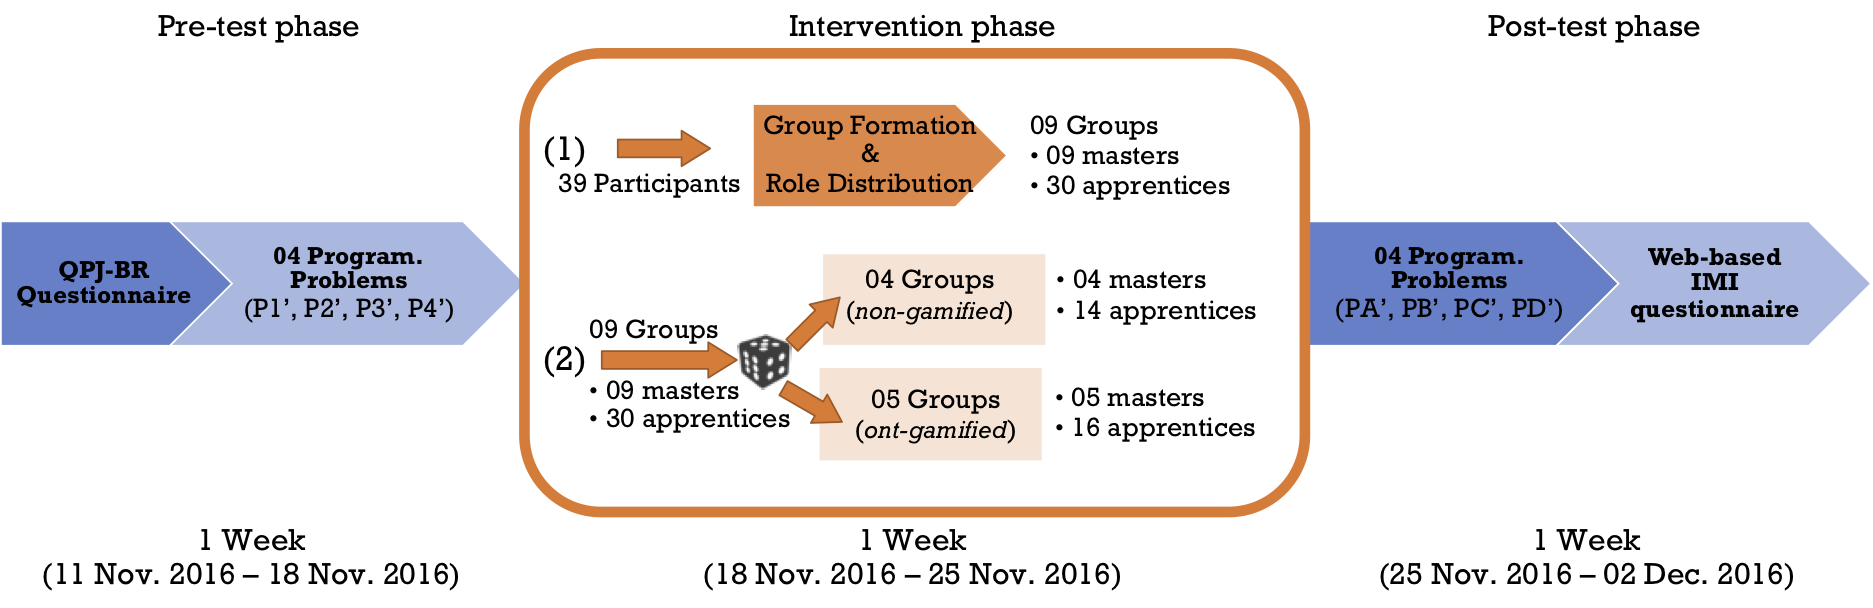
\includegraphics[width=1\textwidth]{images/chap-evaluation/data-collection-procedure-pilot-study.png}
 \fautor
\end{figure}

\textbf{During the pre-test phase (1 week)}, from 11 November 2016 to 18 November 2016, the Web-based QPJ-BR questionnaire has been answered by all the participants through the Moodle platform using the \emph{Questionnaire module}\footnote{Available at the URL: \url{https://github.com/geiser/moodle-mod\_questionnaire}}. During this phase, to gather data related to the skill/knowledge, four programming problem tasks (P1', P2', P3', and P4' - detailed in \autoref{tab:programming-problem-multiple-choice-questionnaires}) have also been solved by the students in the Moodle platform using the VPL module.

\textbf{During the intervention phase (1 week)}, from 18 November 2016 to 25 November 2016, the 39 students participated in either non-gamified CL sessions or ontology-based gamified CL sessions. These students were formed into 9 groups of 4 or 5 members with 9 masters and 30 apprentices assigned according to the theory-driven group formation \cite{IsotaniMizoguchi2008a}. Four of these nine groups participated in non-gamified CL sessions, and five groups participated in ontology-based gamified CL sessions.

The ontological structures to represent \aspas{\emph{Gamified Cognitive Apprenticeship Scenario for Master/Yee Achiever and Apprentice/Yee Achiever}} and \aspas{\emph{Gamified Cognitive Apprenticeship Scenario for Master/Yee Socializer and Apprentice/Yee Socializer}} were used to obtain the ontology-based gamified CL sessions in which:
\begin{itemize}
\item The students who had more liking for achievement-components than positive liking for social-components were assigned to play the \emph{Yee Achiever role} in gamified CL sessions instantiated from the ontological structure \aspas{\emph{Gamified Cognitive Apprenticeship Scenario for Master/Yee Achiever and Apprentice/Yee Achiever}} to support a CL Gameplay experience of \emph{individual competition}.
\item The students who had more positive liking for social-components than positive liking for achievement-components were assigned to play the \emph{Yee Socializer role} in gamified CL sessions instantiated from the ontological structure \aspas{\emph{Gamified Cognitive Apprenticeship Scenario for Master/Yee Socializer and Apprentice/Yee Socializer}} to support a CL Gameplay experience of \emph{cooperative competition}.
\end{itemize}

\textbf{During the post-test phase (1 week)}, from 25 November 2016 to 02 December 2016, to gather data related to the skill/knowledge, four programming problem tasks (PA', PB', PC', and PD' - detailed in \autoref{tab:programming-problem-multiple-choice-questionnaires}) have been solved by the students in the Moodle platform using the VPL module. The students also answered the IMI questionnaire through the Moodle platform using the \emph{Questionnaire module} to gather data related to the participants' intrinsic motivation.

\subsubsection{Execution: First Empirical Study}

The first empirical study was executed over four weeks and four days with the schedule, timing and data collection procedure shown in \autoref{fig:data-collection-procedure-first-study}.

\begin{figure}[htb]
 \caption{Diagram of the schedule, timing and data collection procedure in the first empirical study}
 \label{fig:data-collection-procedure-first-study}
 \centering
 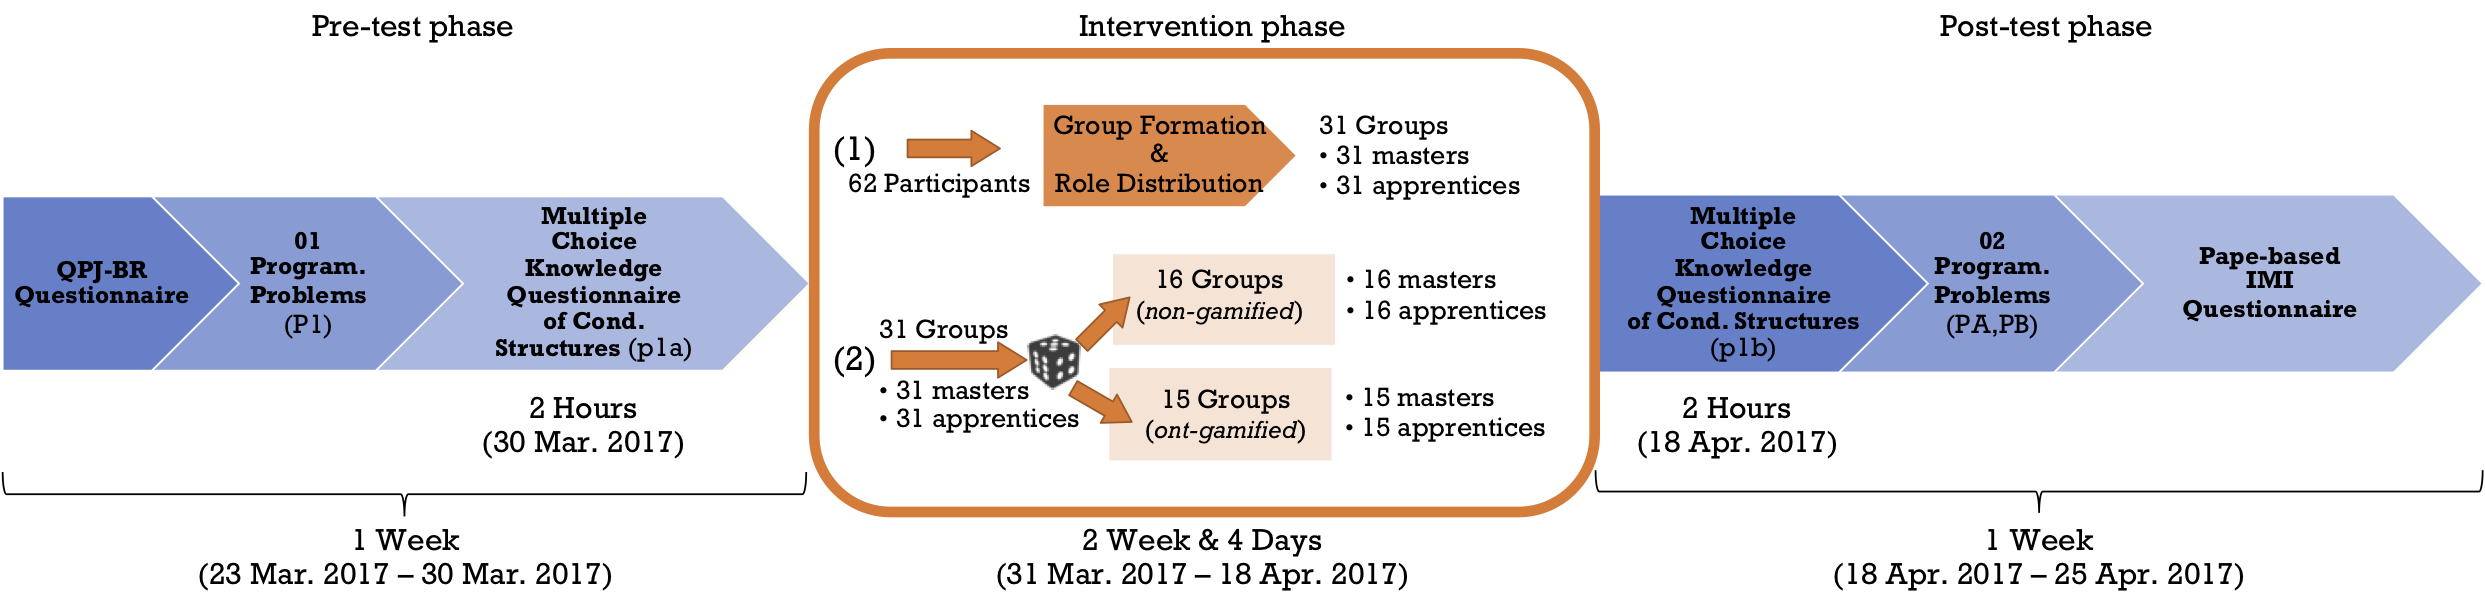
\includegraphics[width=1\textwidth]{images/chap-evaluation/data-collection-procedure-first-study.png}
 \fautor
\end{figure}

\textbf{During the pre-test phase (1 week)}, from 23 March 2017 to 30 March 2017, to gather information of students' preference related to their liking for game-components, the Web-based QPJ-BR questionnaire has been answered by all the participants through the Moodle platform using the \emph{Questionnaire module}. Data related to the participants' initial skill/knowledge were gathered from one programming problem task (P1) and one multiple choice knowledge questionnaire of conditional structures (p1a), both instruments are detailed in \autoref{tab:programming-problem-multiple-choice-questionnaires}. The programming problem task (P1) was solved by the students in the Moodle platform using the \emph{VPL module}, and the students answered the multiple choice knowledge questionnaire (p1a) - during 2 hours on March, 30th - at the classroom in the University of São Paulo as a formative evaluation in the course of Introduction to Computer Science. 

\textbf{During the intervention phase (2 weeks \& 4 days)}, from 31 March 2017 to 18 April 2017, the 62 students participated in either non-gamified CL sessions or ontology-based gamified CL sessions. These students were formed into 31 groups of 2 members with 31 masters and 31 apprentices assigned according to the theory-driven group formation \cite{IsotaniMizoguchi2008a}. Sixteen of thirty one groups participated in non-gamified CL sessions, and fifteen groups participated in ontology-based gamified CL sessions.

The ontological structures to represent \aspas{\emph{Gamified Cognitive Apprenticeship Scenario for Master/Yee Achiever and Apprentice/Yee Achiever}} and \aspas{\emph{Gamified Cognitive Apprenticeship Scenario for Master/Yee Socializer and Apprentice/Yee Socializer}} were used to obtain the ontology-based gamified CL sessions in which:
\begin{itemize}
\item The students who had more liking for achievement-components than positive liking for social-components were assigned to play the \emph{Yee Achiever role} in gamified CL sessions instantiated from the ontological structure \aspas{\emph{Gamified Cognitive Apprenticeship Scenario for Master/Yee Achiever and Apprentice/Yee Achiever}} to support a CL Gameplay experience of \emph{individual competition}.
\item The students who had more positive liking for social-components than positive liking for achievement-components were assigned to play the \emph{Yee Socializer role} in gamified CL sessions instantiated from the ontological structure \aspas{\emph{Gamified Cognitive Apprenticeship Scenario for Master/Yee Socializer and Apprentice/Yee Socializer}} to support a CL Gameplay experience of \emph{cooperative competition}.
\end{itemize}

\textbf{During the post-test phase (1 week)}, from 18 April 2017 to 25 April 2017, to gather data related to the skill/knowledge, the multiple choice knowledge questionnaire of conditional structures (p1b) was answered by the participants - during 2 hours on April, 18th - at the classroom in the University of São Paulo as a formative evaluation in the course of Introduction to Computer Science. Two programming problem tasks (PA, PB - detailed in \autoref{tab:programming-problem-multiple-choice-questionnaires}) have been solved by the students in the Moodle platform using the VPL module. The students also answered the paper-based IMI questionnaire at the classroom in the University of São Paulo to gather data related to the students' intrinsic motivation. 

\subsubsection{Execution: Second Empirical Study}

The second empirical study was executed over four weeks with the schedule, timing and data collection procedure shown in \autoref{fig:data-collection-procedure-second-study}.

\begin{figure}[htb]
 \caption{Diagram of the schedule, timing and data collection procedure in the second empirical study}
 \label{fig:data-collection-procedure-second-study}
 \centering
 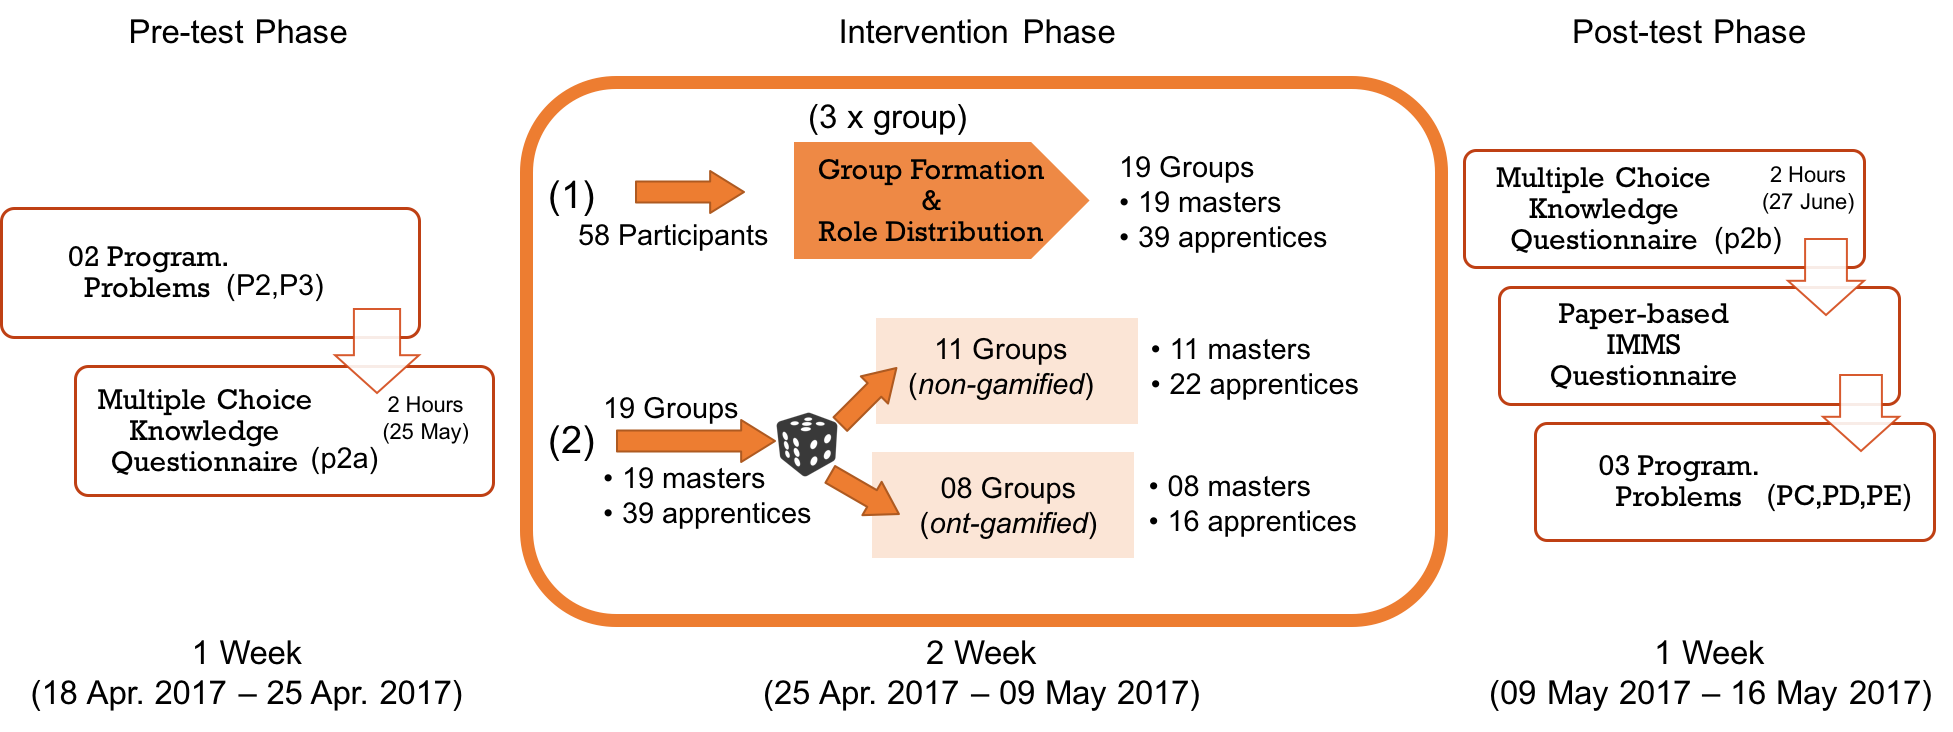
\includegraphics[width=1\textwidth]{images/chap-evaluation/data-collection-procedure-second-study.png}
 \fautor
\end{figure}

\textbf{During the pre-test phase (1 week)}, from 18 April 2017 to 25 April 2017, students' preference related to their liking for game-components were gathered through a paper-based QPJ-BR questionnaire answered by all the students in the Moodle platform using the \emph{Questionnaire module}. Data related to the participants' initial skill/knowledge were gathered from one programming problem task (P2, and P3 - detailed in \autoref{tab:programming-problem-multiple-choice-questionnaires}) and one multiple choice knowledge questionnaire of loop structures (p2a). The students solved the programming problem tasks in the Moodle platform using the \emph{VPL module}, and they answered the multiple choice knowledge questionnaire (p2a) - during 2 hours on April, 25th - at the University of São Paulo as a formative evaluation in the course of Introduction to Computer Science. 

\textbf{During the intervention phase (2 weeks)}, from 25 April 2017 to 9 May 2017, the 58 students participated in either non-gamified CL sessions or ontology-based gamified CL sessions. These students were formed into 19 groups of 3 members with 19 masters and 39 apprentices assigned according to the theory-driven group formation \cite{IsotaniMizoguchi2008a}. Eleven of nineteen groups participated in non-gamified CL sessions, and eight groups participated in ontology-based gamified CL sessions.

The ontological structures to represent \aspas{\emph{Gamified Cognitive Apprenticeship Scenario for Master/Yee Achiever and Apprentice/Yee Achiever}} and \aspas{\emph{Gamified Cognitive Apprenticeship Scenario for Master/Yee Socializer and Apprentice/Yee Socializer}} were used to obtain the ontology-based gamified CL sessions in which:
\begin{itemize}
\item The students who had more liking for achievement-components than positive liking for social-components were assigned to play the \emph{Yee Achiever role} in gamified CL sessions instantiated from the ontological structure \aspas{\emph{Gamified Cognitive Apprenticeship Scenario for Master/Yee Achiever and Apprentice/Yee Achiever}} to support a CL Gameplay experience of \emph{individual competition}.
\item The students who had more positive liking for social-components than positive liking for achievement-components were assigned to play the \emph{Yee Socializer role} in gamified CL sessions instantiated from the ontological structure \aspas{\emph{Gamified Cognitive Apprenticeship Scenario for Master/Yee Socializer and Apprentice/Yee Socializer}} to support a CL Gameplay experience of \emph{cooperative competition}.
\end{itemize}

\textbf{During the post-test phase (1 week)}, from 9 May 2017 to 16 May 2017, to gather data related to the skill/knowledge, the multiple choice knowledge questionnaire of loop structures (p2b) was answered by the students - during 2 hours on May, 9th - at the classroom in the University of São Paulo as a formative evaluation in the course of Introduction to Computer Science. 
Three programming problem tasks (PC, PD, PE - detailed in \autoref{tab:programming-problem-multiple-choice-questionnaires}) have been solved by the students in the Moodle platform using the VPL module. To gather data related to the participants' level of motivation, the students answered the paper-based IMMS questionnaire at the classroom in the University of São Paulo.

\subsubsection{Execution: Third Empirical Study}

The third empirical study was executed over six weeks and three days with the schedule, timing and data collection procedure shown in \autoref{fig:data-collection-procedure-third-study}.

\begin{figure}[htb]
 \caption{Diagram of the schedule, timing and data collection procedure in the third empirical study}
 \label{fig:data-collection-procedure-third-study}
 \centering
 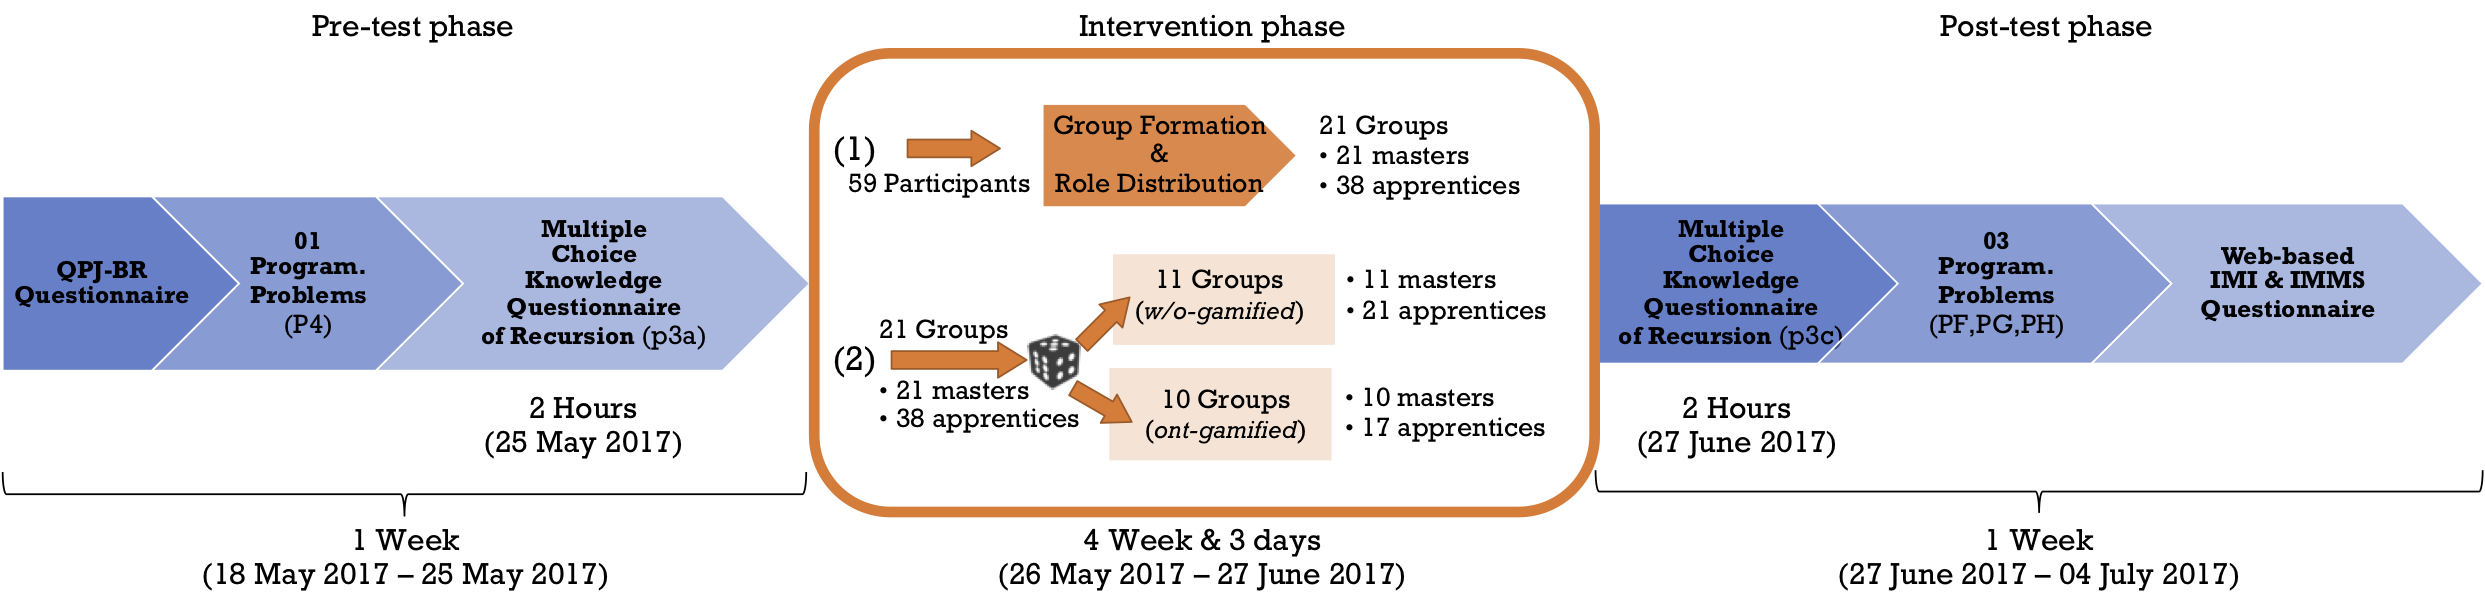
\includegraphics[width=1\textwidth]{images/chap-evaluation/data-collection-procedure-third-study.png}
 \fautor
\end{figure}

\textbf{During the pre-test phase (1 week)}, from 18 May 2017 to 25 May 2017, the Web-based QPJ-BR questionnaire were answered by all the participants through the Moodle platform using the \emph{Questionnaire module}. To gather data related to the skill/knowledge, students solved one programming problem task (P4) in the Moodle platform using the VPL module, and they answered the multiple choice knowledge questionnaire of recursion (p3a) at the classroom in the University of São Paulo - during 2 hours on May 25th.

\textbf{During the intervention phase (4 week \& 3 days)}, from 26 May 2017 to 27 June 2017, the 59 students participated in either ontology-based gamified CL sessions (\emph{ont-gamified} CL sessions) or CL sessions that were gamified without using the support given by the ontology OntoGaCLeS (\emph{w/o-gamified} CL sessions). The students were formed into 21 groups of 2 or 3 members with 21 masters and 38 apprentices assigned according to the theory-driven group formation \cite{IsotaniMizoguchi2008a}. Eleven of twenty-one groups participated in \emph{w/o-gamified} CL sessions, and ten groups participated in \emph{ont-gamified} CL sessions.

The ontological structures to represent \aspas{\emph{Gamified Cognitive Apprenticeship Scenario for Master/Yee Achiever and Apprentice/Yee Achiever}} and \aspas{\emph{Gamified Cognitive Apprenticeship Scenario for Master/Social Achiever and Apprentice/Social Achiever}} were used to obtain the ontology-based gamified CL sessions in which:
\begin{itemize}
\item The students who had liking for achievement-components and did not had liking for social-components were assigned to play the \emph{Yee Achiever role} in gamified CL sessions instantiated from the ontological structure \aspas{\emph{Gamified Cognitive Apprenticeship Scenario for Master/Yee Achiever and Apprentice/Yee Achiever}} to support a CL Gameplay experience of \emph{individual competition}.
\item The students who had positive liking for social-components and achievement-components were assigned to play the \emph{Social Achiever role} in gamified CL sessions instantiated from the ontological structure \aspas{\emph{Gamified Cognitive Apprenticeship Scenario for Master/Social Achiever and Apprentice/Social Achiever}} to support a CL Gameplay experience of \emph{individual and cooperative competition}.
\end{itemize}

\textbf{During the post-test phase (1 week)}, from 27 June 2017 to 04 July 2017, to gather data related to the skill/knowledge, a multiple choice knowledge questionnaire of recursion (p3c) has been answered by the participants at the classroom in University of São Paulo during 2 hours on June 27th. Three programming problem tasks (PF, PG and PH - detailed in \autoref{tab:programming-problem-multiple-choice-questionnaires}) have been solved by the students in the Moodle platform using the VPL module. To gather data related to the students' intrinsic motivation and level of motivation, the students answered the IMI and IMMS questionnaire through the Moodle platform using the \emph{Questionnaire module}.

%% ========================== %%
\subsection{Validity Evaluation}
\label{subsec:validity-evaluation}

The motivation surveys (adapted Portuguese IMI \& IMMS questionnaires) and the data gathered by these instruments to estimate the participants' intrinsic motivation and level of motivation were validated through Confirmatory Factorial Analysis (CFA) and reliability analysis. This validation is detailed in \autoref{appendix:validation-motivation-surveys}, and prior to perform it, the outliers such as careless responses and extreme values were detected and treated as detailed in \autoref{appendix:outliers}. Employing the data gathered by these surveys in the empirical studies, the participants' intrinsic motivation and level of motivation were estimated by means of RSM-based instruments, so that to validate them, their assumptions were checked by test of unidimensionality, test of local independence, and test of monotonicity. The results of these tests are detailed in \autoref{appendix:irt-models}.

To estimate the gains in skill/knowledge from programming problem tasks and multiple choice knowledge questionnaires, the stacking procedures with GPCM were used. Thus, the validation of these measurement instruments were carried out in the GPCM employing the test of unidimensionality, and the test of local independence detailed in \autoref{appendix:irt-models}.

%% ========================== %%
\subsection{Data Analysis Procedure}
\label{sec:evaluation-analysis-procedure}

To measure the students' intrinsic motivation and level of motivation towards their participation in the ontology-based gamified CL sessions, non-gamified CL sessions, and CL session that were gamified without using the support given by the ontology OntoGaCLeS, RSM-based instruments (\autoref{appendix:irt-models}) were used as a psychometric instrument for analyzing the self-reported data collected by the motivation surveys in the empirical studies. The RSM-based instruments are measurement instruments built as Item Response Theory (IRT) models in which the latent trait being measured by the items is estimated in function of rating scale data \cite{George2005}. These instruments are appropriate for the data gathered through the motivation surveys, employed in the empirical studies, in which all the items have a seven-likert scale response format \cite{van2013handbook}.

After having the participants' intrinsic motivation estimates and the level of motivation estimates by means of RSM-based instruments, two-way ANOVA tests have been carried out to compare the effects on the participants' motivation caused by the ontology-based gamified CL sessions. The results on these tests were calculated employing a variation between the types of CL sessions (\emph{ont-gamified} CL sessions, \emph{non-gamified} CL sessions, and \emph{w/o-gamified} CL sessions) and the CL roles played by the participants in these sessions.

To investigate the effect of different types of CL sessions on the learning outcomes, the gains in knowledge/skills of participants have been estimated by stacking the pre-test and post-test data with GPCMs \cite{Wright2003}. \autoref{appendix:irt-models} details the stacked data analyses that were carried out to obtain the gains in knowledge/skills for the empirical studies.
After having these results, two-way ANOVA tests have been run to compare the learning outcomes in the different types of CL sessions and the CL roles played by the participants.

After to carried out the ANOVA tests by evaluating whether there was no significant differences on the participants' motivation and learning outcomes, Spearman's rank-order correlation tests have been run to find out whether the effects of different types of CL sessions on the participants' motivation and learning outcomes were significantly linked.

%%%%%%%%%%%%%%%%%%%%%%%%%%%%%%%%%%%%%%%%%%%%%%%%

\section{Pilot Empirical Study: Data Analysis Results}
\label{sec:pilot-study}

\subsection*{Do the ontology-based gamified CL sessions have positive impacts on the participants' motivation?}

In order to answered this question, two-way between-subjects ANOVA tests were conducted to compare the effects of ontology-based gamified CL sessions (\emph{ont-gamified}) and non-gamified CL sessions (\emph{non-gamified}) on the participants' intrinsic motivation, perceived choice, pressure/tension and effort/importance estimates. The interaction effects between these two types of CL sessions and the CL roles, \emph{Master} and \emph{Apprentice}, are evaluated in these tests. \autoref{tab:two-way-intrinsic-motivation-pilot-study}  shows the results in which there are statistically significant difference at the $0.05$ level for the participants' intrinsic motivation and perceived choice. The effect on the intrinsic motivation for the type of CL session yielded an $F$ ratio of $F(1,26) = 4.702$, $p = 0.039$ with significant differences between non-gamified CL sessions and ont-gamified CL sessions . In relation to the perceived choice, the effect for the type of CL session yielded an $F$ ratio of $F(1,26) = 6.980$, $p = 0.014$, indicating significant differences between non-gamified CL sessions and ont-gamified CL sessions.

%latex.default(result_df, caption = paste("Summary of two-way ANOVA results",     in_title), size = "small", longtable = T, ctable = F, landscape = F,     rowlabel = "", where = "!htbp", file = filename, append = T)%
\setlongtables{\small
\begin{longtable}{lrrrrl}\caption{Two-way ANOVA results for the latent trait estimates of intrinsic motivation, interest/enjoyment, perceived choice, pressure/tension and effort/importance in the pilot empirical study} \tabularnewline
\hline\hline
\multicolumn{1}{l}{}&\multicolumn{1}{c}{Sum Sq}&\multicolumn{1}{c}{Df}&\multicolumn{1}{c}{F value}&\multicolumn{1}{c}{Pr(\textgreater F)}&\multicolumn{1}{c}{Sig}\tabularnewline
\hline
\endfirsthead\caption[]{\em (continued)} \tabularnewline
\hline
\multicolumn{1}{l}{}&\multicolumn{1}{c}{Sum Sq}&\multicolumn{1}{c}{Df}&\multicolumn{1}{c}{F value}&\multicolumn{1}{c}{Pr(\textgreater F)}&\multicolumn{1}{c}{Sig}\tabularnewline
\hline
\endhead
\hline
\multicolumn{6}{r}{\tiny Signif. codes:  0 \aspas{**} 0.01 \aspas{*} 0.05}
\endfoot
\label{tab:two-way-intrinsic-motivation-pilot-study}
%Intrinsic Motivation:(Intercept)&$ 0.042$&$ 1$&$0.082$&$0.777$&\tabularnewline
Intrinsic Motivation:Type&$ 2.397$&$ 1$&$4.702$&$0.039$&*\tabularnewline
%Intrinsic Motivation:CLRole&$ 0.456$&$ 1$&$0.894$&$0.353$&\tabularnewline
Intrinsic Motivation:Type:CLRole&$ 0.080$&$ 1$&$0.156$&$0.696$&\tabularnewline
Intrinsic Motivation:Residuals&$13.254$&$26$&$$&$$&\tabularnewline
%Interest/Enjoyment:(Intercept)&$ 0.483$&$ 1$&$0.208$&$0.652$&$$\tabularnewline
Interest/Enjoyment:Type&$ 8.107$&$ 1$&$3.495$&$0.073$&$$\tabularnewline
%Interest/Enjoyment:CLRole&$ 1.879$&$ 1$&$0.810$&$0.376$&$$\tabularnewline
Interest/Enjoyment:Type:CLRole&$ 0.599$&$ 1$&$0.258$&$0.616$&$$\tabularnewline
Interest/Enjoyment:Residuals&$60.314$&$26$&$$&$$&$$\tabularnewline
%Perceived Choice:(Intercept)&$ 0.103$&$ 1$&$0.195$&$0.663$&\tabularnewline
Perceived Choice:Type&$ 3.675$&$ 1$&$6.980$&$0.014$&*\tabularnewline
%Perceived Choice:CLRole&$ 0.066$&$ 1$&$0.126$&$0.725$&\tabularnewline
Perceived Choice:Type:CLRole&$ 1.050$&$ 1$&$1.994$&$0.170$&\tabularnewline
Perceived Choice:Residuals&$13.689$&$26$&$$&$$&\tabularnewline
%Pressure/Tension:(Intercept)&$ 0.017$&$ 1$&$0.036$&$0.850$&$$\tabularnewline
Pressure/Tension:Type&$ 1.125$&$ 1$&$2.472$&$0.128$&$$\tabularnewline
%Pressure/Tension:CLRole&$ 0.027$&$ 1$&$0.060$&$0.809$&$$\tabularnewline
Pressure/Tension:Type:CLRole&$ 0.012$&$ 1$&$0.026$&$0.874$&$$\tabularnewline
Pressure/Tension:Residuals&$11.838$&$26$&$$&$$&$$\tabularnewline
%Effort/Importance:(Intercept)&$ 0.010$&$ 1$&$0.019$&$0.892$&$$\tabularnewline
Effort/Importance:Type&$ 0.335$&$ 1$&$0.645$&$0.429$&$$\tabularnewline
%Effort/Importance:CLRole&$ 0.068$&$ 1$&$0.130$&$0.721$&$$\tabularnewline
Effort/Importance:Type:CLRole&$ 0.273$&$ 1$&$0.525$&$0.475$&$$\tabularnewline
Effort/Importance:Residuals&$13.516$&$26$&$$&$$&$$\tabularnewline
\hline
\end{longtable}}

Tukey post-hoc comparisons have been run to confirm the significant differences occurred between the types of CL sessions and the CL roles. \autoref{tab:post-hoc-intrinsic-motivation-pilot-study} summarizes the descriptive statistics and the results of post-hoc comparisons. According to these results, the intrinsic motivation of students who participated in ont-gamified CL sessions ($lsmean = 0.419$ \emph{logit}, and $SE = 0.206$) is greater than the intrinsic motivation of students who participated in non-gamified CL sessions ($lsmean = -0.322$ \emph{logit}, and $SE = 0.273$) with a p-adj. value of $0.013$ and Hedges' $g=0.956$ large effect size. The interest/enjoyment of participants in ont-gamified CL sessions ($lsmean = 0.848$ \emph{logit}, and $SE = 0.440$) is greater than the interest/enjoyment of participants in non-gamified CL sessions ($lsmean = -0.515$ \emph{logit}, and $SE = 0.582$) with a p-adj. value of $0.039$ and Hedges' $g=0.780$ medium effect size. In ont-gamified CL sessions, the perceived choice with $lsmean = 0.382$ \emph{logit} and $SE = 0.209$ is significantly greater than the perceived choice in non-gamified CL sessions with $lsmean = -0.535$ \emph{logit} and $SE = 0.277$ at the p-adj. value of $0.031$ and Hedges' $g = 0.814$ large effect size.

Having these results, the null hypothesis, $H_{null,IM,g1}$: \aspas{\emph{There was no significant difference between the intrinsic motivation of students who participated in ontology-based gamified CL sessions and the intrinsic motivation of students who participated in non-gamified CL sessions},} is rejected. Thus, this pilot empirical study becomes an evidence to support the alternative hypothesis, $H_{alt,IM,g1}$: \aspas{\emph{The intrinsic motivation of students who participated in ontology-based gamified CL sessions was greater than the intrinsic motivation of students who participated in non-gamified CL sessions},} with positive impacts in the participants' intrinsic motivation, interest/enjoyment, and perceived choice.

%latex.default(post_hoc_df, caption = paste("Descriptive statistics and Tukey post-hoc test results",     in_title), size = "small", longtable = T, ctable = F, landscape = T,     rowlabel = "", where = "!htbp", file = filename, append = T)%
\setlongtables\begin{landscape}{\scriptsize
\begin{longtable}{lrrrrrrrrrrrll}\caption{Descriptive statistics and Tukey post-hoc test results for the latent trait estimates of intrinsic motivation, interest/enjoyment, perceived choice, pressure/tension and effort/importance in the pilot empirical study} \tabularnewline
\hline\hline
\multicolumn{1}{l}{}&\multicolumn{1}{c}{N}&\multicolumn{1}{c}{mean}&\multicolumn{1}{c}{lsmean}&\multicolumn{1}{c}{SE}&\multicolumn{1}{c}{df}&\multicolumn{1}{c}{lwr.CI}&\multicolumn{1}{c}{upr.CI}&\multicolumn{1}{c}{t.ratio}&\multicolumn{1}{c}{p.value}&\multicolumn{1}{c}{p-adj.}&\multicolumn{1}{c}{g}&\multicolumn{1}{c}{sig}&\multicolumn{1}{c}{mag}\tabularnewline
\hline
\endfirsthead\caption[]{\em (continued)} \tabularnewline
\hline
\multicolumn{1}{l}{}&\multicolumn{1}{c}{N}&\multicolumn{1}{c}{mean}&\multicolumn{1}{c}{lsmean}&\multicolumn{1}{c}{SE}&\multicolumn{1}{c}{df}&\multicolumn{1}{c}{lwr.CI}&\multicolumn{1}{c}{upr.CI}&\multicolumn{1}{c}{t.ratio}&\multicolumn{1}{c}{p.value}&\multicolumn{1}{c}{p-adj.}&\multicolumn{1}{c}{g}&\multicolumn{1}{c}{sig}&\multicolumn{1}{c}{mag}\tabularnewline
\hline
\endhead
\hline
\multicolumn{14}{r}{\tiny Signif. codes:  0 \aspas{**} 0.01 \aspas{*} 0.05} 
\endfoot
\label{tab:post-hoc-intrinsic-motivation-pilot-study}
Intrinsic Motivation:non-gamified&$14$&$-0.389$&$-0.322$&$0.273$&$26$&$-0.882$&$ 0.239$&$$&$$&$$&$$&&\tabularnewline
Intrinsic Motivation:ont-gamified&$16$&$ 0.305$&$ 0.419$&$0.206$&$26$&$-0.004$&$ 0.843$&$$&$$&$$&$$&&\tabularnewline
Intrinsic Motivation:non-gamified - ont-gamified&$30$&$-0.694$&$-0.741$&$0.342$&$$&$-1.231$&$-0.157$&$-2.168$&$0.039$&$0.013$&$-0.956$&*&large\tabularnewline
Intrinsic Motivation:non-gamified.Apprentice&$12$&$-0.416$&$-0.416$&$0.206$&$26$&$-0.839$&$ 0.008$&$$&$$&$$&$$&&\tabularnewline
Intrinsic Motivation:ont-gamified.Apprentice&$12$&$ 0.190$&$ 0.190$&$0.206$&$26$&$-0.233$&$ 0.614$&$$&$$&$$&$$&&\tabularnewline
Intrinsic Motivation:non-gamified.Apprentice - ont-gamified.Apprentice&$24$&$-0.606$&$-0.606$&$0.291$&$$&$-1.406$&$ 0.194$&$-2.079$&$0.048$&$0.186$&$-0.818$&&\tabularnewline
Intrinsic Motivation:non-gamified.Master&$ 2$&$-0.228$&$-0.228$&$0.505$&$26$&$-1.266$&$ 0.810$&$$&$$&$$&$$&&\tabularnewline
Intrinsic Motivation:ont-gamified.Master&$ 4$&$ 0.649$&$ 0.649$&$0.357$&$26$&$-0.085$&$ 1.382$&$$&$$&$$&$$&&\tabularnewline
Intrinsic Motivation:non-gamified.Master - ont-gamified.Master&$ 6$&$-0.876$&$-0.876$&$0.618$&$$&$-2.573$&$ 0.820$&$-1.417$&$0.168$&$0.500$&$-0.991$&&\tabularnewline
\hline

Interest/Enjoyment:non-gamified&$14$&$-0.617$&$-0.515$&$0.582$&$26$&$-1.711$&$ 0.680$&$$&$$&$$&$$&&\tabularnewline
Interest/Enjoyment:ont-gamified&$16$&$ 0.591$&$ 0.848$&$0.440$&$26$&$-0.056$&$ 1.752$&$$&$$&$$&$$&&\tabularnewline
Interest/Enjoyment:non-gamified - ont-gamified&$30$&$-1.208$&$-1.363$&$0.729$&$$&$-2.354$&$-0.063$&$-1.869$&$0.073$&$0.039$&$-0.780$&*&medium\tabularnewline
Interest/Enjoyment:non-gamified.Apprentice&$12$&$-0.658$&$-0.658$&$0.440$&$26$&$-1.562$&$ 0.246$&$$&$$&$$&$$&&\tabularnewline
Interest/Enjoyment:ont-gamified.Apprentice&$12$&$ 0.335$&$ 0.335$&$0.440$&$26$&$-0.569$&$ 1.238$&$$&$$&$$&$$&&\tabularnewline
Interest/Enjoyment:non-gamified.Apprentice - ont-gamified.Apprentice&$24$&$-0.993$&$-0.993$&$0.622$&$$&$-2.698$&$ 0.713$&$-1.596$&$0.123$&$0.398$&$-0.612$&&\tabularnewline
Interest/Enjoyment:non-gamified.Master&$ 2$&$-0.372$&$-0.372$&$1.077$&$26$&$-2.586$&$ 1.841$&$$&$$&$$&$$&&\tabularnewline
Interest/Enjoyment:ont-gamified.Master&$ 4$&$ 1.361$&$ 1.361$&$0.762$&$26$&$-0.204$&$ 2.927$&$$&$$&$$&$$&&\tabularnewline
Interest/Enjoyment:non-gamified.Master - ont-gamified.Master&$ 6$&$-1.734$&$-1.734$&$1.319$&$$&$-5.352$&$ 1.885$&$-1.314$&$0.200$&$0.562$&$-1.100$&&\tabularnewline
\hline

Perceived Choice:non-gamified&$14$&$-0.316$&$-0.535$&$0.277$&$26$&$-1.105$&$ 0.034$&$$&$$&$$&$$&&\tabularnewline
Perceived Choice:ont-gamified&$16$&$ 0.290$&$ 0.382$&$0.209$&$26$&$-0.048$&$ 0.813$&$$&$$&$$&$$&&\tabularnewline
Perceived Choice:non-gamified - ont-gamified&$30$&$-0.607$&$-0.918$&$0.347$&$$&$-1.152$&$-0.061$&$-2.642$&$0.014$&$0.031$&$-0.814$&*&large\tabularnewline
Perceived Choice:non-gamified.Apprentice&$12$&$-0.229$&$-0.229$&$0.209$&$26$&$-0.659$&$ 0.202$&$$&$$&$$&$$&&\tabularnewline
Perceived Choice:ont-gamified.Apprentice&$12$&$ 0.199$&$ 0.199$&$0.209$&$26$&$-0.232$&$ 0.629$&$$&$$&$$&$$&&\tabularnewline
Perceived Choice:non-gamified.Apprentice - ont-gamified.Apprentice&$24$&$-0.427$&$-0.427$&$0.296$&$$&$-1.240$&$ 0.386$&$-1.442$&$0.161$&$0.486$&$-0.557$&&\tabularnewline
Perceived Choice:non-gamified.Master&$ 2$&$-0.842$&$-0.842$&$0.513$&$26$&$-1.897$&$ 0.212$&$$&$$&$$&$$&&\tabularnewline
Perceived Choice:ont-gamified.Master&$ 4$&$ 0.566$&$ 0.566$&$0.363$&$26$&$-0.180$&$ 1.312$&$$&$$&$$&$$&&\tabularnewline
Perceived Choice:non-gamified.Master - ont-gamified.Master&$ 6$&$-1.408$&$-1.408$&$0.628$&$$&$-3.132$&$ 0.316$&$-2.241$&$0.034$&$0.139$&$-1.767$&&\tabularnewline
\hline
\newpage

Pressure/Tension:non-gamified&$14$&$ 0.238$&$ 0.285$&$0.258$&$26$&$-0.245$&$0.814$&$$&$$&$$&$$&$$&$$\tabularnewline
Pressure/Tension:ont-gamified&$16$&$-0.230$&$-0.223$&$0.195$&$26$&$-0.624$&$0.177$&$$&$$&$$&$$&$$&$$\tabularnewline
Pressure/Tension:non-gamified - ont-gamified&$30$&$ 0.468$&$ 0.508$&$0.323$&$$&$-0.040$&$0.976$&$1.572$&$0.128$&$0.069$&$0.699$&$$&$$\tabularnewline
Pressure/Tension:non-gamified.Apprentice&$12$&$ 0.219$&$ 0.219$&$0.195$&$26$&$-0.181$&$0.620$&$$&$$&$$&$$&$$&$$\tabularnewline
Pressure/Tension:ont-gamified.Apprentice&$12$&$-0.237$&$-0.237$&$0.195$&$26$&$-0.637$&$0.164$&$$&$$&$$&$$&$$&$$\tabularnewline
Pressure/Tension:non-gamified.Apprentice - ont-gamified.Apprentice&$24$&$ 0.456$&$ 0.456$&$0.275$&$$&$-0.300$&$1.212$&$1.656$&$0.110$&$0.366$&$0.624$&$$&$$\tabularnewline
Pressure/Tension:non-gamified.Master&$ 2$&$ 0.350$&$ 0.350$&$0.477$&$26$&$-0.631$&$1.331$&$$&$$&$$&$$&$$&$$\tabularnewline
Pressure/Tension:ont-gamified.Master&$ 4$&$-0.210$&$-0.210$&$0.337$&$26$&$-0.903$&$0.484$&$$&$$&$$&$$&$$&$$\tabularnewline
Pressure/Tension:non-gamified.Master - ont-gamified.Master&$ 6$&$ 0.560$&$ 0.560$&$0.584$&$$&$-1.044$&$2.163$&$0.958$&$0.347$&$0.774$&$0.950$&$$&$$\tabularnewline
\hline

Effort/Importance:non-gamified&$14$&$ 0.028$&$ 0.162$&$0.275$&$26$&$-0.404$&$0.728$&$$&$$&$$&$$&$$&$$\tabularnewline
Effort/Importance:ont-gamified&$16$&$-0.084$&$-0.115$&$0.208$&$26$&$-0.543$&$0.313$&$$&$$&$$&$$&$$&$$\tabularnewline
Effort/Importance:non-gamified - ont-gamified&$30$&$ 0.112$&$ 0.277$&$0.345$&$$&$-0.430$&$0.654$&$0.803$&$0.429$&$0.674$&$0.155$&$$&$$\tabularnewline
Effort/Importance:non-gamified.Apprentice&$12$&$-0.025$&$-0.025$&$0.208$&$26$&$-0.453$&$0.403$&$$&$$&$$&$$&$$&$$\tabularnewline
Effort/Importance:ont-gamified.Apprentice&$12$&$-0.052$&$-0.052$&$0.208$&$26$&$-0.480$&$0.376$&$$&$$&$$&$$&$$&$$\tabularnewline
Effort/Importance:non-gamified.Apprentice - ont-gamified.Apprentice&$24$&$ 0.027$&$ 0.027$&$0.294$&$$&$-0.780$&$0.835$&$0.092$&$0.927$&$1.000$&$0.037$&$$&$$\tabularnewline
Effort/Importance:non-gamified.Master&$ 2$&$ 0.349$&$ 0.349$&$0.510$&$26$&$-0.699$&$1.397$&$$&$$&$$&$$&$$&$$\tabularnewline
Effort/Importance:ont-gamified.Master&$ 4$&$-0.178$&$-0.178$&$0.361$&$26$&$-0.919$&$0.563$&$$&$$&$$&$$&$$&$$\tabularnewline
Effort/Importance:non-gamified.Master - ont-gamified.Master&$ 6$&$ 0.527$&$ 0.527$&$0.624$&$$&$-1.186$&$2.240$&$0.844$&$0.406$&$0.833$&$0.545$&$$&$$\tabularnewline
\hline
\end{longtable}}\end{landscape}

\newpage
\subsection*{Do the ontology-based gamified CL sessions positively affect on the participants' learning outcomes?}

In order to answer this question, two-way between-subjects ANOVA tests were run to compare the effects of ontology-based gamified CL sessions (\emph{ont-gamified}) and non-gamified CL sessions (\emph{non-gamified}) on the gains in skill/knowledge estimates. These tests evaluated the interaction effects between these two types of CL sessions and the two CL roles: \emph{Master} and \emph{Apprentice}. The results of these tests are shown in \autoref{tab:two-way-learning-outcomes-pilot-study} in which there are not statistically significant difference at the $0.05$ level for the gains in skill/knowledge estimates for the \aspas{\emph{signed-up students}} (SignedUpPs) and \aspas{\emph{students with effective participation}} (EffectivePs).
\begin{itemize}
\item 
\emph{Signed-up students} (SignedUpPs) were students enrolled in the course, and that were participants in the CL sessions
\item
\emph{Students with effective participation} (EffectivePs) were signed-up students who had a complete, semicomplete or incomplete participation level in the CL sessions. It means that they were students with at least interacted one time in the CL session (non-gamified CL session or ont-gamified CL session) with other member of CL group.
\end{itemize}

%latex.default(result_df, caption = paste("Summary of two-way ANOVA results",     in_title), size = "small", longtable = T, ctable = F, landscape = F,     rowlabel = "", where = "!htbp", file = filename, append = T)%
\setlongtables{\small
\begin{longtable}{lrrrrl}\caption{Two-way ANOVA results for the gains in skill/knowledge estimates in the pilot empirical study} \tabularnewline
\hline\hline
\multicolumn{1}{l}{}&\multicolumn{1}{c}{Sum Sq}&\multicolumn{1}{c}{Df}&\multicolumn{1}{c}{F value}&\multicolumn{1}{c}{Pr(\textgreater F)}&\multicolumn{1}{c}{Sig}\tabularnewline
\hline
\endfirsthead\caption[]{\em (continued)} \tabularnewline
\hline
\multicolumn{1}{l}{}&\multicolumn{1}{c}{Sum Sq}&\multicolumn{1}{c}{Df}&\multicolumn{1}{c}{F value}&\multicolumn{1}{c}{Pr(\textgreater F)}&\multicolumn{1}{c}{Sig}\tabularnewline
\hline
\endhead
\hline
\multicolumn{6}{r}{\tiny Signif. codes:  0 \aspas{**} 0.01 \aspas{*} 0.05}
\endfoot
\label{tab:two-way-learning-outcomes-pilot-study} 
%SignedUpPs:(Intercept)&$147.269$&$ 1$&$32.624$&$0.000$&\tabularnewline
SignedUpPs:Type&$  0.432$&$ 1$&$ 0.096$&$0.759$&\tabularnewline
%SignedUpPs:CLRole&$ 48.137$&$ 1$&$10.664$&$0.003$&**\tabularnewline
SignedUpPs:Type:CLRole&$  3.485$&$ 1$&$ 0.772$&$0.388$&\tabularnewline
SignedUpPs:Residuals&$117.368$&$26$&$$&$$&\tabularnewline
%EffectivePs:(Intercept)&$126.330$&$ 1$&$35.770$&$0.000$&\tabularnewline
EffectivePs:Type&$  3.087$&$ 1$&$ 0.874$&$0.363$&\tabularnewline
%EffectivePs:CLRole&$ 42.192$&$ 1$&$11.947$&$0.003$&**\tabularnewline
EffectivePs:Type:CLRole&$  0.427$&$ 1$&$ 0.121$&$0.732$&\tabularnewline
EffectivePs:Residuals&$ 60.040$&$17$&$$&$$&\tabularnewline
\hline
\end{longtable}}

To confirm the significant differences occurred between the types of CL sessions and the CL roles, Tukey post-hoc comparisons have been run, and \autoref{tab:post-hoc-learning-outcomes-pilot-study} summarizes the results of post-hoc comparisons and the descriptive statistics. Although the gains in skill/knowledge estimates for students with effective participation in ont-gamified CL sessions were greater than the gains in skill/knowledge estimates for students with effective participation in non-gamified CL sessions, there were not significant differences in the gains in skill/knowledge of signed-up students and students with effective participation. Thus, the null hypothesis, $H_{null,GSK,g1}$: \aspas{\emph{There was no significant difference between the gains in skill/knowledge obtained by students who participated in ontology-based gamified CL sessions and the gains in skill/knowledge obtained by students who participated in non-gamified CL sessions},} is not rejected.

%latex.default(post_hoc_df, caption = paste("Descriptive statistics and Tukey post-hoc test results",     in_title), size = "small", longtable = T, ctable = F, landscape = T,     rowlabel = "", where = "!htbp", file = filename, append = T)%
\setlongtables\begin{landscape}{\scriptsize
\begin{longtable}{lrrrrrrrrrrrrr}\caption{Descriptive statistics and Tukey post-hoc test results for the gains in skill/knowledge estimates in the pilot empirical study} \tabularnewline
\hline\hline
\multicolumn{1}{l}{}&\multicolumn{1}{c}{N}&\multicolumn{1}{c}{mean}&\multicolumn{1}{c}{lsmean}&\multicolumn{1}{c}{SE}&\multicolumn{1}{c}{df}&\multicolumn{1}{c}{lwr.CI}&\multicolumn{1}{c}{upr.CI}&\multicolumn{1}{c}{t.ratio}&\multicolumn{1}{c}{p.value}&\multicolumn{1}{c}{p.ajd}&\multicolumn{1}{c}{g}&\multicolumn{1}{c}{sig}&\multicolumn{1}{c}{mag}\tabularnewline
\hline
\endfirsthead\caption[]{\em (continued)} \tabularnewline
\hline
\multicolumn{1}{l}{}&\multicolumn{1}{c}{N}&\multicolumn{1}{c}{mean}&\multicolumn{1}{c}{lsmean}&\multicolumn{1}{c}{SE}&\multicolumn{1}{c}{df}&\multicolumn{1}{c}{lwr.CI}&\multicolumn{1}{c}{upr.CI}&\multicolumn{1}{c}{t.ratio}&\multicolumn{1}{c}{p.value}&\multicolumn{1}{c}{p.ajd}&\multicolumn{1}{c}{g}&\multicolumn{1}{c}{sig}&\multicolumn{1}{c}{mag}\tabularnewline
\hline
\endhead
\hline
\multicolumn{14}{r}{\tiny Signif. codes:  0 \aspas{**} 0.01 \aspas{*} 0.05} 
\endfoot
\label{tab:post-hoc-learning-outcomes-pilot-study}
SignedUpPs:non-gamified&$14$&$ 3.768$&$ 2.705$&$0.692$&$26$&$ 1.282$&$4.127$&$$&$$&$$&$$&$$&$$\tabularnewline
SignedUpPs:ont-gamified&$16$&$ 2.829$&$ 2.427$&$0.573$&$26$&$ 1.249$&$3.604$&$$&$$&$$&$$&$$&$$\tabularnewline
SignedUpPs:non-gamified - ont-gamified&$30$&$ 0.940$&$ 0.278$&$0.898$&$$&$-0.659$&$2.538$&$ 0.309$&$0.759$&$0.238$&$ 0.376$&$$&$$\tabularnewline
SignedUpPs:non-gamified.Apprentice&$11$&$ 4.566$&$ 4.566$&$0.641$&$26$&$ 3.249$&$5.883$&$$&$$&$$&$$&$$&$$\tabularnewline
SignedUpPs:ont-gamified.Apprentice&$11$&$ 3.499$&$ 3.499$&$0.641$&$26$&$ 2.182$&$4.816$&$$&$$&$$&$$&$$&$$\tabularnewline
SignedUpPs:non-gamified.Apprentice - ont-gamified.Apprentice&$22$&$ 1.067$&$ 1.067$&$0.906$&$$&$-1.418$&$3.553$&$ 1.178$&$0.249$&$0.646$&$ 0.517$&$$&$$\tabularnewline
SignedUpPs:non-gamified.Master&$ 3$&$ 0.843$&$ 0.843$&$1.227$&$26$&$-1.678$&$3.365$&$$&$$&$$&$$&$$&$$\tabularnewline
SignedUpPs:ont-gamified.Master&$ 5$&$ 1.355$&$ 1.355$&$0.950$&$26$&$-0.599$&$3.308$&$$&$$&$$&$$&$$&$$\tabularnewline
SignedUpPs:non-gamified.Master - ont-gamified.Master&$ 8$&$-0.511$&$-0.511$&$1.552$&$$&$-4.768$&$3.745$&$-0.330$&$0.744$&$0.987$&$-0.176$&$$&$$\tabularnewline


EffectivePs:non-gamified&$ 8$&$ 2.535$&$ 2.196$&$0.686$&$17$&$ 0.749$&$3.644$&$$&$$&$$&$$&$$&$$\tabularnewline
EffectivePs:ont-gamified&$13$&$ 3.392$&$ 3.010$&$0.536$&$17$&$ 1.880$&$4.140$&$$&$$&$$&$$&$$&$$\tabularnewline
EffectivePs:non-gamified - ont-gamified&$21$&$-0.858$&$-0.814$&$0.871$&$$&$-2.639$&$0.924$&$-0.935$&$0.363$&$0.324$&$-0.346$&$$&$$\tabularnewline
EffectivePs:non-gamified.Apprentice&$ 5$&$ 3.550$&$ 3.550$&$0.840$&$17$&$ 1.776$&$5.323$&$$&$$&$$&$$&$$&$$\tabularnewline
EffectivePs:ont-gamified.Apprentice&$ 8$&$ 4.666$&$ 4.666$&$0.664$&$17$&$ 3.264$&$6.068$&$$&$$&$$&$$&$$&$$\tabularnewline
EffectivePs:non-gamified.Apprentice - ont-gamified.Apprentice&$13$&$-1.116$&$-1.116$&$1.071$&$$&$-4.162$&$1.929$&$-1.042$&$0.312$&$0.728$&$-0.740$&$$&$$\tabularnewline
EffectivePs:non-gamified.Master&$ 3$&$ 0.843$&$ 0.843$&$1.085$&$17$&$-1.446$&$3.132$&$$&$$&$$&$$&$$&$$\tabularnewline
EffectivePs:ont-gamified.Master&$ 5$&$ 1.355$&$ 1.355$&$0.840$&$17$&$-0.419$&$3.128$&$$&$$&$$&$$&$$&$$\tabularnewline
EffectivePs:non-gamified.Master - ont-gamified.Master&$ 8$&$-0.511$&$-0.511$&$1.372$&$$&$-4.413$&$3.390$&$-0.373$&$0.714$&$0.982$&$-0.176$&$$&$$\tabularnewline

\hline
\end{longtable}}\end{landscape}

\newpage
\subsection*{Are the participants' motivation and learning outcomes linked in either the non-gamified CL sessions or the ontology-based gamified CL sessions?}

Spearman's rank-order correlation tests were run to determine the relationship between the motivation and learning outcomes obtained by signed-up students (SignedUpPs) and students with effective participation (EffectivePs) in the ontology-based gamified CL sessions (\emph{ont-gamified}) and the non-gamified CL sessions (\emph{non-gamified}). 
\autoref{tab:correlation-matrices-pilot-study} shows the results of the correlation tests and their p-values in which the gains in skill/knowledge estimates were used as learning outcome measurement, and the intrinsic motivation, interest/enjoyment, perceived choice, pressure/tension and effort/importance estimates were used as motivation measurement.

According to these results, there was not significant correlation between the participants' motivation and learning outcomes in the non-gamified CL sessions and ont-gamified CL sessions. Thus, the null hypothesis, $H_{null,\rho,g1}$: \aspas{\emph{There was no significant correlation between the participants' motivation and their gains in skill/knowledge in either the non-gamified CL sessions or the ontology-based gamified CL sessions},} is not rejected.

%latex.default(round(M, 4), caption = paste("Correlation matrix",     "of", mod$title, in_title), size = "small", longtable = T,     ctable = F, landscape = T, insert.bottom = paste("method: ",         mod$method), where = "!htbp", file = filename, append = T)%
\setlongtables{\scriptsize
\begin{longtable}{lR{1.5cm}R{1.5cm}R{1.5cm}R{1.5cm}R{1.5cm}}\caption{Correlation matrices and their p-values for the motivation and learning outcomes of participants in the pilot empirical study} \tabularnewline
\hline\hline
\multicolumn{1}{l}{Gains in Skill/Knowledge}&\multicolumn{1}{R{1.5cm}}{\mbox{Intrinsic} \mbox{Motivation}}&\multicolumn{1}{R{1.5cm}}{\mbox{Interest}/ \mbox{Enjoyment}}&\multicolumn{1}{R{1.5cm}}{\mbox{Perceived} \mbox{Choice}}&\multicolumn{1}{R{1.5cm}}{\mbox{Pressure}/ \mbox{Tension}}&\multicolumn{1}{R{1.5cm}}{\mbox{Effort}/ \mbox{Importance}}\tabularnewline
\hline
\endfirsthead\caption[]{\em (continued)} \tabularnewline
\hline
\multicolumn{1}{l}{Gains in Skill/Knowledge}&\multicolumn{1}{R{1.5cm}}{\mbox{Intrinsic} \mbox{Motivation}}&\multicolumn{1}{R{1.5cm}}{\mbox{Interest}/ \mbox{Enjoyment}}&\multicolumn{1}{R{1.5cm}}{\mbox{Perceived} \mbox{Choice}}&\multicolumn{1}{R{1.5cm}}{\mbox{Pressure}/ \mbox{Tension}}&\multicolumn{1}{R{1.5cm}}{\mbox{Effort}/ \mbox{Importance}}\tabularnewline
\hline
\endhead
\hline
\multicolumn{6}{r}{\tiny method:  spearman}\tabularnewline
\endfoot
\label{tab:correlation-matrices-pilot-study}
SignedUpPs:non-gamified&$-0.3500$&$-0.2368$&$-0.0700$&$-0.0948$&$0.0112$\tabularnewline
 &$(0.24)$&$(0.43)$&$(0.82)$&$(0.75)$&$(0.97)$\tabularnewline
SignedUpPs:ont-gamified&$-0.3771$&$-0.4327$&$-0.3872$&$ 0.3131$&$0.3067$\tabularnewline
 &$(0.18)$&$(0.12)$&$(0.17)$&$(0.27)$&$(0.28)$\tabularnewline
SignedUpPs:non-gamified.Apprentice&$-0.3149$&$-0.1628$&$-0.3466$&$-0.0419$&$0.2150$\tabularnewline
 &$(0.34)$&$(0.63)$&$(0.29)$&$(0.90)$&$(0.52)$\tabularnewline
SignedUpPs:ont-gamified.Apprentice&$-0.0486$&$-0.1094$&$-0.0973$&$ 0.2294$&$0.5368$\tabularnewline
  &$(0.89)$&$(0.76)$&$(0.78)$&$(0.52)$&$(0.10)$\tabularnewline
\hline
EffectivePs:non-gamified&$ 0.0721$&$0.3784$&$ 0.3945$&$ 0.1802$&$ 0.1182$\tabularnewline
 &$(0.87)$&$(0.40)$&$(0.38)$&$(0.69)$&$(0.80)$\tabularnewline
EffectivePs:ont-gamified&$-0.4772$&$-0.5123$&$-0.3996$&$ 0.4137$&$0.3215$\tabularnewline
 &$(0.11)$&$(0.08)$&$(0.19)$&$(0.18)$&$(0.30)$\tabularnewline
EffectivePs:non-gamified.Apprentice&$ 0.1026$&$ 0.5643$&$-0.7105$&$ 0.4104$&$ 0.6579$\tabularnewline
 &$(0.86)$&$(0.32)$&$(0.17)$&$(0.49)$&$(0.22)$\tabularnewline
EffectivePs:ont-gamified.Apprentice&$-0.3114$&$-0.1796$&$-0.0599$&$ 0.4424$&$0.4817$\tabularnewline
 &$(0.45)$&$(0.67)$&$(0.88)$&$(0.27)$&$(0.22)$\tabularnewline
\hline
\end{longtable}}


\subsection*{Do the ontology-based gamified CL sessions have positive effects on the percentages of participation per groups?}

In order to answer this question, Mann-Whitney's U tests have been run on  different percentages of participation per group in ontology-based gamified CL sessions (\emph{ont-gamified}) and non-gamified CL sessions (\emph{non-gamified}). These percentages were: the percentage of students per groups having any participation (\emph{PctHavingParticipation} - refers to complete, semicomplete and incomplete participation level), the percentage of students per groups having an adequate participation (\emph{PctAdequateParticipation} - refers to complete and semicomplete participation level), the percentage of students per groups having incomplete participation (\emph{PctIncompleteParticipation} - refers to incomplete and none participation level), and the percentage of students per groups without participation (\emph{PctWithoutParticipation} - refers to none participation level).

The participation levels are defined as:
\begin{itemize}
\item
\emph{None participation level}: when the student did not interact with others in CL sessions
\item
\emph{Incomplete participation level}: when the student interacted in CL sessions, but he/she did not complete all the necessary interactions
\item
\emph{Semicomplete participation level}: when the student interacted in CL sessions carried out all the necessary interactions, but he/she did not respond to all requests made by others
\item
\emph{Complete participation level}: when the student interacted in CL sessions performing all the necessary interactions, and he/she responds to all requests made by others
\end{itemize}

\autoref{tab:mann-whitney-result-participation} shows the results of Mann-Whitney's U tests in which there were significant differences for all the percentages of participation per groups with exception of the percentage of students per groups having an adequate participation. According to these results, the percentage of students per groups having any participation in ont-gamified CL sessions ($median = 0.50$) was greater than the percentage of students per groups having any participation in non-gamified CL sessions ($median = 0.40$). This result indicates a significant difference with values of $U = 10.5$, $Z= -1.78$, \emph{p-value}$ = 0.035$ and $r = 0.477$ (medium effect size). The percentage of students per groups having an incomplete participation in ont-gamified CL sessions ($median = 0.25$) was significantly less than the percentage of students per groups having an incomplete participation in non-gamified CL sessions ($median = 0.60$) with values of $U = 21.0$, $Z= 1.79$, \emph{p-value}$ = 0.048$ and $r = 0.567$ (large effect size). Finally, with values of $U = 12.0$, $Z= 2.16$, \emph{p-value}$ = 0.029$ and $r = 0.816$ (large effect size), the percentage of students per groups without participation in ont-gamified CL sessions ($median = 0.25$) was significantly less than the percentage of students per groups without participation in non-gamified CL sessions ($median = 0.60$).

%latex.default(result_wilcoxon_df, caption = paste("Full descriptive statistic of the pair wilcoxon analysis",     in_title), size = "scriptsize", longtable = T, ctable = F,     landscape = T, rowlabel = "", where = "!htbp", file = filename,     append = T)%
\setlongtables%\begin{landscape}
{\scriptsize
\begin{longtable}{llrrrrrrrrll}\caption{Mann-Whitney's U results for 
the pct. of participation per groups
in the pilot empirical study} \tabularnewline
\hline\hline
\multicolumn{1}{l}{}&\multicolumn{1}{c}{Type}&\multicolumn{1}{c}{N}&\multicolumn{1}{c}{Med}&\multicolumn{1}{c}{Mean.R}&\multicolumn{1}{c}{U}&\multicolumn{1}{c}{Z}&\multicolumn{1}{c}{p.value}&\multicolumn{1}{c}{r}&\multicolumn{1}{c}{mag}&\multicolumn{1}{c}{Sig}\tabularnewline
\hline
\endfirsthead\caption[]{\em (continued)} \tabularnewline
\hline
\multicolumn{1}{l}{}&\multicolumn{1}{c}{Type}&\multicolumn{1}{c}{N}&\multicolumn{1}{c}{Med}&\multicolumn{1}{c}{Mean.R}&\multicolumn{1}{c}{U}&\multicolumn{1}{c}{Z}&\multicolumn{1}{c}{p.value}&\multicolumn{1}{c}{r}&\multicolumn{1}{c}{mag}&\multicolumn{1}{c}{Sig}\tabularnewline
\hline
\endhead
\hline
\multicolumn{11}{r}{\tiny Signif. codes:  0 \aspas{**} 0.01 \aspas{*} 0.05}
\endfoot
\label{tab:mann-whitney-result-participation}
PctHavingParticipation&non-gamified&$6$&$0.40$&$5.25$&$10.5$&$-1.78$&$0.035$&$0.477$&med&*\tabularnewline
PctHavingParticipation&ont-gamified&$8$&$0.50$&$9.19$&$10.5$&$-1.78$&$0.035$&$0.477$&med&*\tabularnewline
PctAdequateParticipation&non-gamified&$4$&$0.40$&$4.12$&$ 6.5$&$-1.45$&$0.082$&$0.436$&med&\tabularnewline
PctAdequateParticipation&ont-gamified&$7$&$0.50$&$7.07$&$ 6.5$&$-1.45$&$0.082$&$0.436$&med&\tabularnewline
PctIncompleteParticipation&non-gamified&$5$&$0.60$&$7.20$&$21.0$&$ 1.79$&$0.048$&$0.567$&larg&*\tabularnewline
PctIncompleteParticipation&ont-gamified&$5$&$0.25$&$3.80$&$21.0$&$ 1.79$&$0.048$&$0.567$&larg&*\tabularnewline
PctWithoutParticipation&non-gamified&$3$&$0.60$&$6.00$&$12.0$&$ 2.16$&$0.029$&$0.816$&larg&*\tabularnewline
PctWithoutParticipation&ont-gamified&$4$&$0.25$&$2.50$&$12.0$&$ 2.16$&$0.029$&$0.816$&larg&*\tabularnewline
\hline
\end{longtable}}%\end{landscape}

Based on these results, the null hypothesis, $H_{null,Pct,g1}$: \aspas{\emph{
There was no significant difference between the percentages of participation per groups in ontology-based gamified CL sessions and the percentages of participation per groups in non-gamified CL sessions},} is rejected. In this sense, this empirical study becomes an evidence to support the alternative hypothesis, $H_{alt,Pct,g1}$: \aspas{\emph{
The percentages of participation per groups in ontology-based gamified CL sessions are better than the percentage of participation per groups in non-gamified CL sessions},} increasing the percentage of students per groups having any participation, and reducing the percentage of students per groups having an incomplete participation and without participation. 

%%%%%%%%%%%%%%%%%%%%%%%%%%%%%%%%%%%%%%%%%%%%%%%%
\section{First Empirical Study: Data Analysis Results}
\label{sec:first-study}

\subsection*{Do the ontology-based gamified CL sessions have positive impacts on the participants' motivation?}

In order to answer this question, 
two-way ANOVA tests have been run to compare the effects of ontology-based gamified CL sessions (\emph{ont-gamified}) and non-gamified CL sessions (\emph{non-gamified}) on the participants' intrinsic motivation, interest/enjoyment, perceived choice, pressure/tension and effort/importance.
\autoref{tab:two-way-intrinsic-motivation-first-study} shows the results of the ANOVA tests, and 
according to these results, there were statistically significant difference at the $0.05$ level for the participants' intrinsic motivation, interest/enjoyment, pressure/tension and effort/importance. On the participants' intrinsic motivation, the effect for the type of CL session yielded a $F$ ratio of $F(1,56) = 8.103$ and $p = 0.006$ indicating significant differences between non-gamified CL sessions and ont-gamified CL sessions. The effect on the participants' perceived choice for the type of CL session yielded a $F$ ratio of $F(1,56) = 7.885$ and $p = 0.007$ indicating significant differences between non-gamified CL sessions and ont-gamified CL sessions. On the participants' pressure/tension, the effect for the type of CL session and CL roles yielded a $F$ ratio of $F(1,56) = 6.151$ and $p = 0.016$ indicating significant differences between the pressure/tension of apprentices in non-gamified CL sessions and the pressure/tension of apprentices in ont-gamified CL sessions. The effect on the effort/importance for the type of CL session yielded a $F$ ratio of $F(1,56) = 4.303$ and $p = 0.043$ indicating significant differences between non-gamified CL sessions and ont-gamified CL sessions.


%latex.default(result_df, caption = paste("Summary of two-way ANOVA results",     in_title), size = "small", longtable = T, ctable = F, landscape = F,     rowlabel = "", where = "!htbp", file = filename, append = T)%
\setlongtables{\small
\begin{longtable}{lrrrrl}\caption{Two-way ANOVA for the latent trait estimates of intrinsic motivation, interest/enjoyment, perceived choice, pressure/tension and effort/importance in the first empirical study} \tabularnewline
\hline\hline
\multicolumn{1}{l}{}&\multicolumn{1}{c}{Sum Sq}&\multicolumn{1}{c}{Df}&\multicolumn{1}{c}{F value}&\multicolumn{1}{c}{Pr(\textgreater F)}&\multicolumn{1}{c}{Sig}\tabularnewline
\hline
\endfirsthead\caption[]{\em (continued)} \tabularnewline
\hline
\multicolumn{1}{l}{}&\multicolumn{1}{c}{Sum Sq}&\multicolumn{1}{c}{Df}&\multicolumn{1}{c}{F value}&\multicolumn{1}{c}{Pr(\textgreater F)}&\multicolumn{1}{c}{Sig}\tabularnewline
\hline
\endhead
\hline
\multicolumn{6}{r}{\tiny Signif. codes:  0 \aspas{**} 0.01 \aspas{*} 0.05}
\endfoot
\label{tab:two-way-intrinsic-motivation-first-study}
%Intrinsic Motivation:(Intercept)&$ 0.579$&$ 1$&$1.520$&$0.223$&\tabularnewline
Intrinsic Motivation:Type&$ 3.087$&$ 1$&$8.103$&$0.006$&**\tabularnewline
%Intrinsic Motivation:CLRole&$ 0.064$&$ 1$&$0.168$&$0.683$&\tabularnewline
Intrinsic Motivation:Type:CLRole&$ 0.020$&$ 1$&$0.053$&$0.819$&\tabularnewline
Intrinsic Motivation:Residuals&$21.333$&$56$&$$&$$&\tabularnewline
%Interest/Enjoyment:(Intercept)&$ 0.421$&$ 1$&$0.419$&$0.520$&$$\tabularnewline
Interest/Enjoyment:Type&$ 0.946$&$ 1$&$0.942$&$0.336$&$$\tabularnewline
%Interest/Enjoyment:CLRole&$ 0.268$&$ 1$&$0.267$&$0.607$&$$\tabularnewline
Interest/Enjoyment:Type:CLRole&$ 2.003$&$ 1$&$1.993$&$0.164$&$$\tabularnewline
Interest/Enjoyment:Residuals&$52.258$&$52$&$$&$$&$$\tabularnewline
%Perceived Choice:(Intercept)&$ 0.016$&$ 1$&$0.020$&$0.889$&\tabularnewline
Perceived Choice:Type&$ 6.371$&$ 1$&$7.885$&$0.007$&**\tabularnewline
%Perceived Choice:CLRole&$ 0.229$&$ 1$&$0.283$&$0.597$&\tabularnewline
Perceived Choice:Type:CLRole&$ 0.050$&$ 1$&$0.061$&$0.805$&\tabularnewline
Perceived Choice:Residuals&$45.244$&$56$&$$&$$&\tabularnewline
%Pressure/Tension:(Intercept)&$ 5.506$&$ 1$&$5.333$&$0.025$&\tabularnewline
Pressure/Tension:Type&$ 2.428$&$ 1$&$2.352$&$0.131$&\tabularnewline
%Pressure/Tension:CLRole&$ 0.011$&$ 1$&$0.011$&$0.918$&\tabularnewline
Pressure/Tension:Type:CLRole&$ 6.351$&$ 1$&$6.151$&$0.016$&*\tabularnewline
Pressure/Tension:Residuals&$57.815$&$56$&$$&$$&\tabularnewline
%Effort/Importance:(Intercept)&$ 0.078$&$ 1$&$0.086$&$0.770$&\tabularnewline
Effort/Importance:Type&$ 3.861$&$ 1$&$4.303$&$0.043$&*\tabularnewline
%Effort/Importance:CLRole&$ 2.374$&$ 1$&$2.646$&$0.109$&\tabularnewline
Effort/Importance:Type:CLRole&$ 0.799$&$ 1$&$0.891$&$0.349$&\tabularnewline
Effort/Importance:Residuals&$50.244$&$56$&$$&$$&\tabularnewline
\hline
\end{longtable}}

Tukey post-hoc comparisons were run to confirm the significant differences in the participants' motivation of ANOVA tests. \autoref{tab:post-hoc-intrinsic-motivation-first-study} shows the results of the post-hoc comparisons in which the intrinsic motivation of participants in ont-gamified CL sessions ($lsmean=0.129$ \emph{logit}, and $SE = 0.113$) is greater than the intrinsic motivation of participants in non-gamified CL sessions ($lsmean=-0.325$ \emph{logit}, and $SE = 0.113$) with a p-adj. value of $0.006$ and Hedges' $g=0.743$ medium effect size. The perceived choice of participants in ont-gamified CL sessions ($lsmean=0.310$ \emph{logit}, and $SE = 0.164$) is greater than the perceived choice of participants in non-gamified CL sessions ($lsmean=-0.343$ \emph{logit}, and $SE = 0.164$) with a p-adj. value of $0.007$ and Hedges' $g=0.724$ medium effect size. The pressure/tension of apprentices in ont-gamified CL sessions ($lsmean=-0.237$ \emph{logit}, and $SE = 0.262$) is less than apprentices in non-gamified CL sessions ($lsmean=0.817$ \emph{logit}, and $SE = 0.272$) with a p-adj. value of $0.035$ and Hedges' $g=0.964$ large effect size. The participants' effort/importance in ont-gamified CL sessions ($lsmean=0.218$ \emph{logit}, and $SE = 0.173$) is greater than the participants' effort/importance in non-gamified CL sessions ($lsmean=-0.290$ \emph{logit}, and $SE = 0.173$) with a p-adj. value of $0.035$ and Hedges' $g=0.544$ medium effect size.

According to the results obtained in the two-way ANOVA tests and Tukey post-hoc comparisons, the null hypothesis, $H_{null,IM,g1}$: \aspas{\emph{There was no significant difference between the intrinsic motivation of students who participated in ontology-based gamified CL sessions and the intrinsic motivation of students who participated in non-gamified CL sessions},} is rejected becoming this empirical study an evidence to support the alternative hypothesis, $H_{alt,IM,g1}$: \aspas{\emph{The intrinsic motivation of students who participated in ontology-based gamified CL sessions was greater than the intrinsic motivation of students who participated in non-gamified CL sessions},} with positive impacts in the intrinsic motivation, perceived choice, pressure/tension (of apprentices), and effort/importance.

%latex.default(post_hoc_df, caption = paste("Descriptive statistics and Tukey post-hoc test results",     in_title), size = "small", longtable = T, ctable = F, landscape = T,     rowlabel = "", where = "!htbp", file = filename, append = T)%
\setlongtables\begin{landscape}{\scriptsize
\begin{longtable}{lrrrrrrrrrrrll}\caption{Descriptive statistics and Tukey post-hoc test results for the latent trait estimates of intrinsic motivation, interest/enjoyment, perceived choice, pressure/tension and effort/importance in the first empirical study} \tabularnewline
\hline\hline
\multicolumn{1}{l}{}&\multicolumn{1}{c}{N}&\multicolumn{1}{c}{mean}&\multicolumn{1}{c}{lsmean}&\multicolumn{1}{c}{SE}&\multicolumn{1}{c}{df}&\multicolumn{1}{c}{lwr.CI}&\multicolumn{1}{c}{upr.CI}&\multicolumn{1}{c}{t.ratio}&\multicolumn{1}{c}{p.value}&\multicolumn{1}{c}{p-adj.}&\multicolumn{1}{c}{g}&\multicolumn{1}{c}{sig}&\multicolumn{1}{c}{mag}\tabularnewline
\hline
\endfirsthead\caption[]{\em (continued)} \tabularnewline
\hline
\multicolumn{1}{l}{}&\multicolumn{1}{c}{N}&\multicolumn{1}{c}{mean}&\multicolumn{1}{c}{lsmean}&\multicolumn{1}{c}{SE}&\multicolumn{1}{c}{df}&\multicolumn{1}{c}{lwr.CI}&\multicolumn{1}{c}{upr.CI}&\multicolumn{1}{c}{t.ratio}&\multicolumn{1}{c}{p.value}&\multicolumn{1}{c}{p-adj.}&\multicolumn{1}{c}{g}&\multicolumn{1}{c}{sig}&\multicolumn{1}{c}{mag}\tabularnewline
\hline
\endhead
\hline
\multicolumn{14}{r}{\tiny Signif. codes:  0 \aspas{**} 0.01 \aspas{*} 0.05}
\endfoot
\label{tab:post-hoc-intrinsic-motivation-first-study}
Intrinsic Motivation:non-gamified&$30$&$-0.329$&$-0.325$&$0.113$&$56$&$-0.552$&$-0.099$&$$&$$&$$&$$&&\tabularnewline
Intrinsic Motivation:ont-gamified&$30$&$ 0.129$&$ 0.129$&$0.113$&$56$&$-0.097$&$ 0.354$&$$&$$&$$&$$&&\tabularnewline
Intrinsic Motivation:non-gamified - ont-gamified&$60$&$-0.458$&$-0.454$&$0.160$&$$&$-0.777$&$-0.138$&$-2.847$&$0.006$&$0.006$&$-0.743$&**&medium\tabularnewline
Intrinsic Motivation:non-gamified.Apprentice&$14$&$-0.274$&$-0.274$&$0.165$&$56$&$-0.605$&$ 0.056$&$$&$$&$$&$$&&\tabularnewline
Intrinsic Motivation:ont-gamified.Apprentice&$15$&$ 0.143$&$ 0.143$&$0.159$&$56$&$-0.176$&$ 0.462$&$$&$$&$$&$$&&\tabularnewline
Intrinsic Motivation:non-gamified.Apprentice - ont-gamified.Apprentice&$29$&$-0.418$&$-0.418$&$0.229$&$$&$-1.025$&$ 0.190$&$-1.820$&$0.074$&$0.275$&$-0.583$&&\tabularnewline
Intrinsic Motivation:non-gamified.Master&$16$&$-0.376$&$-0.376$&$0.154$&$56$&$-0.686$&$-0.067$&$$&$$&$$&$$&&\tabularnewline
Intrinsic Motivation:ont-gamified.Master&$15$&$ 0.114$&$ 0.114$&$0.159$&$56$&$-0.205$&$ 0.434$&$$&$$&$$&$$&&\tabularnewline
Intrinsic Motivation:non-gamified.Master - ont-gamified.Master&$31$&$-0.491$&$-0.491$&$0.222$&$$&$-1.078$&$ 0.097$&$-2.212$&$0.031$&$0.132$&$-0.896$&&\tabularnewline
\hline

Interest/Enjoyment:non-gamified&$28$&$-0.217$&$-0.217$&$0.189$&$52$&$-0.597$&$0.163$&$$&$$&$$&$$&$$&$$\tabularnewline
Interest/Enjoyment:ont-gamified&$28$&$ 0.062$&$ 0.043$&$0.190$&$52$&$-0.338$&$0.424$&$$&$$&$$&$$&$$&$$\tabularnewline
Interest/Enjoyment:non-gamified - ont-gamified&$56$&$-0.279$&$-0.260$&$0.268$&$$&$-0.816$&$0.259$&$-0.970$&$0.336$&$0.303$&$-0.274$&$$&$$\tabularnewline
Interest/Enjoyment:non-gamified.Apprentice&$14$&$-0.097$&$-0.097$&$0.268$&$52$&$-0.635$&$0.441$&$$&$$&$$&$$&$$&$$\tabularnewline
Interest/Enjoyment:ont-gamified.Apprentice&$13$&$-0.215$&$-0.215$&$0.278$&$52$&$-0.773$&$0.343$&$$&$$&$$&$$&$$&$$\tabularnewline
Interest/Enjoyment:non-gamified.Apprentice - ont-gamified.Apprentice&$27$&$ 0.118$&$ 0.118$&$0.386$&$$&$-0.906$&$1.143$&$ 0.307$&$0.760$&$0.990$&$ 0.106$&$$&$$\tabularnewline
Interest/Enjoyment:non-gamified.Master&$14$&$-0.337$&$-0.337$&$0.268$&$52$&$-0.875$&$0.201$&$$&$$&$$&$$&$$&$$\tabularnewline
Interest/Enjoyment:ont-gamified.Master&$15$&$ 0.302$&$ 0.302$&$0.259$&$52$&$-0.217$&$0.821$&$$&$$&$$&$$&$$&$$\tabularnewline
Interest/Enjoyment:non-gamified.Master - ont-gamified.Master&$29$&$-0.639$&$-0.639$&$0.373$&$$&$-1.628$&$0.350$&$-1.715$&$0.092$&$0.326$&$-0.678$&$$&$$\tabularnewline
\hline

Perceived Choice:non-gamified&$30$&$-0.340$&$-0.343$&$0.164$&$56$&$-0.672$&$-0.013$&$$&$$&$$&$$&&\tabularnewline
Perceived Choice:ont-gamified&$30$&$ 0.310$&$ 0.310$&$0.164$&$56$&$-0.019$&$ 0.639$&$$&$$&$$&$$&&\tabularnewline
Perceived Choice:non-gamified - ont-gamified&$60$&$-0.650$&$-0.652$&$0.232$&$$&$-1.115$&$-0.185$&$-2.808$&$0.007$&$0.007$&$-0.724$&**&medium\tabularnewline
Perceived Choice:non-gamified.Apprentice&$14$&$-0.376$&$-0.376$&$0.240$&$56$&$-0.857$&$ 0.106$&$$&$$&$$&$$&&\tabularnewline
Perceived Choice:ont-gamified.Apprentice&$15$&$ 0.219$&$ 0.219$&$0.232$&$56$&$-0.246$&$ 0.684$&$$&$$&$$&$$&&\tabularnewline
Perceived Choice:non-gamified.Apprentice - ont-gamified.Apprentice&$29$&$-0.595$&$-0.595$&$0.334$&$$&$-1.479$&$ 0.290$&$-1.781$&$0.080$&$0.293$&$-0.617$&&\tabularnewline
Perceived Choice:non-gamified.Master&$16$&$-0.310$&$-0.310$&$0.225$&$56$&$-0.760$&$ 0.141$&$$&$$&$$&$$&&\tabularnewline
Perceived Choice:ont-gamified.Master&$15$&$ 0.401$&$ 0.401$&$0.232$&$56$&$-0.064$&$ 0.865$&$$&$$&$$&$$&&\tabularnewline
Perceived Choice:non-gamified.Master - ont-gamified.Master&$31$&$-0.710$&$-0.710$&$0.323$&$$&$-1.565$&$ 0.145$&$-2.198$&$0.032$&$0.136$&$-0.802$&&\tabularnewline
\newpage

Pressure/Tension:non-gamified&$30$&$ 0.484$&$ 0.505$&$0.186$&$56$&$ 0.132$&$0.877$&$$&$$&$$&$$&&\tabularnewline
Pressure/Tension:ont-gamified&$30$&$ 0.102$&$ 0.102$&$0.186$&$56$&$-0.270$&$0.473$&$$&$$&$$&$$&&\tabularnewline
Pressure/Tension:non-gamified - ont-gamified&$60$&$ 0.382$&$ 0.403$&$0.263$&$$&$-0.144$&$0.908$&$ 1.534$&$0.131$&$0.151$&$ 0.358$&&\tabularnewline
Pressure/Tension:non-gamified.Apprentice&$14$&$ 0.817$&$ 0.817$&$0.272$&$56$&$ 0.273$&$1.361$&$$&$$&$$&$$&&\tabularnewline
Pressure/Tension:ont-gamified.Apprentice&$15$&$-0.237$&$-0.237$&$0.262$&$56$&$-0.763$&$0.288$&$$&$$&$$&$$&&\tabularnewline
Pressure/Tension:non-gamified.Apprentice - ont-gamified.Apprentice&$29$&$ 1.054$&$ 1.054$&$0.378$&$$&$ 0.054$&$2.054$&$ 2.792$&$0.007$&$0.035$&$ 0.964$&*&large\tabularnewline
Pressure/Tension:non-gamified.Master&$16$&$ 0.193$&$ 0.193$&$0.254$&$56$&$-0.316$&$0.701$&$$&$$&$$&$$&&\tabularnewline
Pressure/Tension:ont-gamified.Master&$15$&$ 0.441$&$ 0.441$&$0.262$&$56$&$-0.084$&$0.967$&$$&$$&$$&$$&&\tabularnewline
Pressure/Tension:non-gamified.Master - ont-gamified.Master&$31$&$-0.249$&$-0.249$&$0.365$&$$&$-1.216$&$0.718$&$-0.681$&$0.499$&$0.904$&$-0.249$&&\tabularnewline
\hline

Effort/Importance:non-gamified&$30$&$-0.311$&$-0.290$&$0.173$&$56$&$-0.637$&$ 0.057$&$$&$$&$$&$$&&\tabularnewline
Effort/Importance:ont-gamified&$30$&$ 0.218$&$ 0.218$&$0.173$&$56$&$-0.128$&$ 0.564$&$$&$$&$$&$$&&\tabularnewline
Effort/Importance:non-gamified - ont-gamified&$60$&$-0.529$&$-0.508$&$0.245$&$$&$-1.019$&$-0.039$&$-2.074$&$0.043$&$0.035$&$-0.544$&*&medium\tabularnewline
Effort/Importance:non-gamified.Apprentice&$14$&$ 0.025$&$ 0.025$&$0.253$&$56$&$-0.482$&$ 0.532$&$$&$$&$$&$$&&\tabularnewline
Effort/Importance:ont-gamified.Apprentice&$15$&$ 0.302$&$ 0.302$&$0.245$&$56$&$-0.188$&$ 0.792$&$$&$$&$$&$$&&\tabularnewline
Effort/Importance:non-gamified.Apprentice - ont-gamified.Apprentice&$29$&$-0.277$&$-0.277$&$0.352$&$$&$-1.209$&$ 0.655$&$-0.786$&$0.435$&$0.860$&$-0.260$&&\tabularnewline
Effort/Importance:non-gamified.Master&$16$&$-0.605$&$-0.605$&$0.237$&$56$&$-1.079$&$-0.130$&$$&$$&$$&$$&&\tabularnewline
Effort/Importance:ont-gamified.Master&$15$&$ 0.134$&$ 0.134$&$0.245$&$56$&$-0.356$&$ 0.624$&$$&$$&$$&$$&&\tabularnewline
Effort/Importance:non-gamified.Master - ont-gamified.Master&$31$&$-0.739$&$-0.739$&$0.340$&$$&$-1.640$&$ 0.162$&$-2.171$&$0.034$&$0.144$&$-0.839$&&\tabularnewline
\hline
\end{longtable}}\end{landscape}

\newpage
\subsection*{Do the ontology-based gamified CL sessions positively affect on the participants' learning outcomes?}

In order to answer this question, two-way between-subjects ANOVA tests were conducted to compare the effects of non-gamified CL sessions (\emph{non-gamified}) and ontology-based gamified CL sessions (\emph{ont-gamified}) on the gains in skill/knowledge estimates. The results of these tests are indicated in \autoref{tab:anova-learning-outcomes-first} in which there was a significant difference on the gains in skill/knowledge estimates of students with effective participation in CL sessions (EffectivePs). This significant difference is indicated for the interaction between the type of CL session and CL roles with a $F$ ratio of $F(1,42) = 7.609$ and $p = 0.009$ (EffectivePs:Type:CLRole).

\setlongtables{\small
\begin{longtable}{lrrrrl}\caption{Two-way ANOVA results for the gains in skill/knowledge estimates in the first empirical study} \tabularnewline
\hline\hline
\multicolumn{1}{l}{}&\multicolumn{1}{c}{Sum Sq}&\multicolumn{1}{c}{Df}&\multicolumn{1}{c}{F value}&\multicolumn{1}{c}{Pr(\textgreater F)}&\multicolumn{1}{c}{Sig}\tabularnewline
\hline
\endfirsthead\caption[]{\em (continued)} \tabularnewline
\hline
\multicolumn{1}{l}{}&\multicolumn{1}{c}{Sum Sq}&\multicolumn{1}{c}{Df}&\multicolumn{1}{c}{F value}&\multicolumn{1}{c}{Pr(\textgreater F)}&\multicolumn{1}{c}{Sig}\tabularnewline
\hline
\endhead
\hline
\multicolumn{6}{r}{\tiny Signif. codes:  0 \aspas{**} 0.01 \aspas{*} 0.05}
\endfoot
\label{tab:anova-learning-outcomes-first}
%Type.(Intercept)&$9.866$&$ 1$&$291.364$&$0.000$&\tabularnewline
SignedUpPs:Type&$0.031$&$ 1$&$  0.927$&$0.340$&\tabularnewline
%SignedUpPs:CLRole&$1.321$&$ 1$&$ 39.020$&$0.000$&**\tabularnewline
SignedUpPs:Type:CLRole&$0.002$&$ 1$&$  0.067$&$0.796$&\tabularnewline
SignedUpPs:Residuals&$1.693$&$50$&$$&$$&\tabularnewline
%EffectivePs:(Intercept)&$10.287$&$ 1$&$228.937$&$0.000$&\tabularnewline
EffectivePs:Type&$ 0.095$&$ 1$&$  2.124$&$0.152$&\tabularnewline
%EffectivePs:CLRole&$ 0.280$&$ 1$&$  6.242$&$0.016$&*\tabularnewline
EffectivePs:Type:CLRole&$ 0.342$&$ 1$&$  7.609$&$0.009$&**\tabularnewline
EffectivePs:Residuals&$ 1.887$&$42$&$$&$$&\tabularnewline
\hline
\end{longtable}}

\autoref{tab:learning-outcomes-post-hoc-tukey-first-study} shown the Tukey post-hoc comparisons results for the first empirical study. These comparisons have been run to confirm the significant differences found by the ANOVA tests on the gains in skill/knowledge for the types of CL sessions and the CL roles. According to these results, for the master students with effective participation, the gains in skill/knowledge in ont-gamified CL sessions ($lsmean = 0.271$ \emph{logit}, and $SE = 0.057$) were significantly less than the gains in skill/knowledge in non-gamified CL sessions ($lsmean = 0.542$ \emph{logit}, and $SE = 0.075$) with a p-adj. value of $0.030$ and Hedges' $g = 1.108$ large effect size.

Having the results of Tukey post-hoc comparisons, the null hypothesis, $H_{null,GSK,g1}$: \aspas{\emph{There was no significant difference between the gains in skill/knowledge obtained by students who participated in ontology-based gamified CL sessions and the gains in skill/knowledge obtained by students who participated in non-gamified CL sessions},} is rejected. However, the first empirical study is not an evidence to support 
the alternative hypothesis, $H_{alt,GSK,g1}$: \aspas{\emph{The gains in skill/knowledge obtained by students who participated in ontology-based gamified CL sessions was greater than the gains in skill/knowledge obtained by students who participated in non-gamified CL sessions},}
because the gains in skill/knowledge estimates of master students in non-gamified CL sessions were significantly greater than the gains in skill/knowledge of master students in ont-gamified CL sessions.

%latex.default(post_hoc_df, caption = paste("Descriptive statistics and Tukey post-hoc test results",     in_title), size = "small", longtable = T, ctable = F, landscape = T,     rowlabel = "", where = "!htbp", file = filename, append = T)%
\setlongtables\begin{landscape}{\scriptsize
\begin{longtable}{lrrrrrrrrrrrrr}\caption{Descriptive statistics and Tukey post-hoc test results for the gains in skill/knowledge estimates in the first empirical study} \tabularnewline
\hline\hline
\multicolumn{1}{l}{}&\multicolumn{1}{c}{N}&\multicolumn{1}{c}{mean}&\multicolumn{1}{c}{lsmean}&\multicolumn{1}{c}{SE}&\multicolumn{1}{c}{df}&\multicolumn{1}{c}{lwr.CI}&\multicolumn{1}{c}{upr.CI}&\multicolumn{1}{c}{t.ratio}&\multicolumn{1}{c}{p.value}&\multicolumn{1}{c}{p.ajd}&\multicolumn{1}{c}{g}&\multicolumn{1}{c}{sig}&\multicolumn{1}{c}{mag}\tabularnewline
\hline
\endfirsthead\caption[]{\em (continued)} \tabularnewline
\hline
\multicolumn{1}{l}{}&\multicolumn{1}{c}{N}&\multicolumn{1}{c}{mean}&\multicolumn{1}{c}{lsmean}&\multicolumn{1}{c}{SE}&\multicolumn{1}{c}{df}&\multicolumn{1}{c}{lwr.CI}&\multicolumn{1}{c}{upr.CI}&\multicolumn{1}{c}{t.ratio}&\multicolumn{1}{c}{p.value}&\multicolumn{1}{c}{p.ajd}&\multicolumn{1}{c}{g}&\multicolumn{1}{c}{sig}&\multicolumn{1}{c}{mag}\tabularnewline
\hline
\endhead
\hline
\multicolumn{14}{r}{\tiny Signif. codes:  0 \aspas{**} 0.01 \aspas{*} 0.05}
\endfoot
\label{tab:learning-outcomes-post-hoc-tukey-first-study}
SignedUpPs:non-gamified&$24$&$ 0.419$&$ 0.407$&$0.038$&$50$&$ 0.331$&$0.482$&$$&$$&$$&$$&$$&$$\tabularnewline
SignedUpPs:ont-gamified&$30$&$ 0.455$&$ 0.455$&$0.034$&$50$&$ 0.388$&$0.523$&$$&$$&$$&$$&$$&$$\tabularnewline
SignedUpPs:non-gamified - ont-gamified&$54$&$-0.036$&$-0.049$&$0.050$&$$&$-0.137$&$0.065$&$-0.963$&$0.340$&$0.478$&$-0.147$&$$&$$\tabularnewline
SignedUpPs:non-gamified.Apprentice&$13$&$ 0.558$&$ 0.558$&$0.051$&$50$&$ 0.455$&$0.660$&$$&$$&$$&$$&$$&$$\tabularnewline
SignedUpPs:ont-gamified.Apprentice&$15$&$ 0.620$&$ 0.620$&$0.048$&$50$&$ 0.524$&$0.715$&$$&$$&$$&$$&$$&$$\tabularnewline
SignedUpPs:non-gamified.Apprentice - ont-gamified.Apprentice&$28$&$-0.062$&$-0.062$&$0.070$&$$&$-0.247$&$0.124$&$-0.885$&$0.380$&$0.813$&$-0.376$&$$&$$\tabularnewline
SignedUpPs:non-gamified.Master&$11$&$ 0.255$&$ 0.255$&$0.055$&$50$&$ 0.144$&$0.367$&$$&$$&$$&$$&$$&$$\tabularnewline
SignedUpPs:ont-gamified.Master&$15$&$ 0.291$&$ 0.291$&$0.048$&$50$&$ 0.196$&$0.386$&$$&$$&$$&$$&$$&$$\tabularnewline
SignedUpPs:non-gamified.Master - ont-gamified.Master&$26$&$-0.036$&$-0.036$&$0.073$&$$&$-0.230$&$0.159$&$-0.486$&$0.629$&$0.962$&$-0.166$&$$&$$\tabularnewline


EffectivePs:non-gamified&$18$&$ 0.532$&$ 0.533$&$0.050$&$42$&$ 0.432$&$0.635$&$$&$$&$$&$$&&\tabularnewline
EffectivePs:ont-gamified&$28$&$ 0.439$&$ 0.439$&$0.040$&$42$&$ 0.359$&$0.520$&$$&$$&$$&$$&&\tabularnewline
EffectivePs:non-gamified - ont-gamified&$46$&$ 0.093$&$ 0.094$&$0.064$&$$&$-0.036$&$0.222$&$ 1.457$&$0.152$&$0.155$&$ 0.369$&&\tabularnewline
EffectivePs:non-gamified.Apprentice&$10$&$ 0.525$&$ 0.525$&$0.067$&$42$&$ 0.390$&$0.660$&$$&$$&$$&$$&&\tabularnewline
EffectivePs:ont-gamified.Apprentice&$14$&$ 0.608$&$ 0.608$&$0.057$&$42$&$ 0.494$&$0.723$&$$&$$&$$&$$&&\tabularnewline
EffectivePs:non-gamified.Apprentice - ont-gamified.Apprentice&$24$&$-0.084$&$-0.084$&$0.088$&$$&$-0.318$&$0.151$&$-0.953$&$0.346$&$0.777$&$-0.429$&&\tabularnewline
EffectivePs:non-gamified.Master&$ 8$&$ 0.542$&$ 0.542$&$0.075$&$42$&$ 0.390$&$0.693$&$$&$$&$$&$$&&\tabularnewline
EffectivePs:ont-gamified.Master&$14$&$ 0.271$&$ 0.271$&$0.057$&$42$&$ 0.156$&$0.385$&$$&$$&$$&$$&&\tabularnewline
EffectivePs:non-gamified.Master - ont-gamified.Master&$22$&$ 0.271$&$ 0.271$&$0.094$&$$&$ 0.020$&$0.522$&$ 2.885$&$0.006$&$0.030$&$ 1.108$&*&large\tabularnewline

\hline
\end{longtable}}\end{landscape}

\newpage
\subsection*{Are the participants' motivation and learning outcomes linked in either the non-gamified CL sessions or the ontology-based gamified CL sessions?}

Spearman's rank-order correlation tests were run to determine the relationship between the motivation and learning outcomes obtained by signed-up students and students with effective participation in the ontology-based gamified CL sessions (\emph{ont-gamified}) and the non-gamified CL sessions (\emph{non-gamified}). The results of these tests and their p-values are shown in \autoref{tab:correlation-matrices-first-study} in which the gains in skill/knowledge estimates were used as learning outcome measurement, and the intrinsic motivation, interest/enjoyment, perceived choice, pressure/tension and effort/importance estimates were used as motivation measurement. 

%latex.default(round(M, 4), caption = paste("Correlation matrix",     "of", mod$title, in_title), size = "small", longtable = T,     ctable = F, landscape = T, insert.bottom = paste("method: ",         mod$method), where = "!htbp", file = filename, append = T)%
\setlongtables%\begin{landscape}
{\scriptsize
\begin{longtable}{lR{1.5cm}R{1.5cm}R{1.5cm}R{1.5cm}R{1.5cm}}\caption{Correlation matrices and their p-values for the motivation and learning outcomes of participants in the first empirical study}\tabularnewline
\hline\hline
\multicolumn{1}{l}{Gains in Skill/Knowledge}&\multicolumn{1}{R{1.5cm}}{\mbox{Intrinsic} \mbox{Motivation}}&\multicolumn{1}{R{1.5cm}}{\mbox{Interest}/ \mbox{Enjoyment}}&\multicolumn{1}{R{1.5cm}}{\mbox{Perceived} \mbox{Choice}}&\multicolumn{1}{R{1.5cm}}{\mbox{Pressure}/ \mbox{Tension}}&\multicolumn{1}{R{1.5cm}}{\mbox{Effort}/ \mbox{Importance}}\tabularnewline
\hline
\endfirsthead\caption[]{\em (continued)} \tabularnewline
\hline
\multicolumn{1}{l}{Gains in Skill/Knowledge}&\multicolumn{1}{R{1.5cm}}{\mbox{Intrinsic} \mbox{Motivation}}&\multicolumn{1}{R{1.5cm}}{\mbox{Interest}/ \mbox{Enjoyment}}&\multicolumn{1}{R{1.5cm}}{\mbox{Perceived} \mbox{Choice}}&\multicolumn{1}{R{1.5cm}}{\mbox{Pressure}/ \mbox{Tension}}&\multicolumn{1}{R{1.5cm}}{\mbox{Effort}/ \mbox{Importance}}\tabularnewline
\hline
\endhead
\hline
\multicolumn{6}{r}{\tiny method:  spearman}\tabularnewline
\endfoot
\label{tab:correlation-matrices-first-study}
SignedUpPs:non-gamified&$ 0.0600$&$ 0.1896$&$-0.1347$&$ 0.1505$&$ 0.2631$\tabularnewline
 &$(0.79)$&$(0.39)$&$(0.55)$&$(0.50)$&$(0.23)$\tabularnewline
SignedUpPs:ont-gamified&$-0.1594$&$-0.3114$&$-0.1451$&$-0.0789$&$ 0.0066$\tabularnewline
 &$(0.41)$&$(0.10)$&$(0.46)$&$(0.68)$&$(0.97)$\tabularnewline
SignedUpPs:non-gamified.Master&$-0.1500$&$-0.2510$&$-0.4790$&$-0.1881$&$ 0.3521$\tabularnewline
 &$(0.70)$&$(0.51)$&$(0.19)$&$(0.62)$&$(0.35)$\tabularnewline
SignedUpPs:ont-gamified.Master&$-0.0215$&$-0.1213$&$-0.0898$&$-0.1618$&$-0.2577$\tabularnewline
 &$(0.93)$&$(0.66)$&$(0.75)$&$(0.56)$&$(0.35)$\tabularnewline
SignedUpPs:non-gamified.Apprentice&$ 0.1699$&$ 0.3899$&$ 0.0419$&$-0.1537$&$-0.1136$\tabularnewline
 &$(0.57)$&$(0.18)$&$(0.89)$&$(0.61)$&$(0.71)$\tabularnewline
SignedUpPs:ont-gamified.Apprentice&$-0.4451$&$-0.3333$&$-0.3435$&$ 0.2918$&$ 0.1365$\tabularnewline
 &$(0.12)$&$(0.26)$&$(0.25)$&$(0.33)$&$(0.65)$\tabularnewline
\hline

EffectivePs:non-gamified&$ 0.2962$&$ 0.1404$&$ 0.1912$&$ 0.0052$&$0.4230$\tabularnewline
 &$(0.23)$&$(0.57)$&$(0.44)$&$(0.98)$&$(0.08)$\tabularnewline
EffectivePs:ont-gamified&$-0.1621$&$-0.3131$&$-0.2139$&$-0.0644$&$ 0.0658$\tabularnewline
 &$(0.42)$&$(0.11)$&$(0.29)$&$(0.75)$&$(0.74)$\tabularnewline
EffectivePs:non-gamified.Master&$ 0.3095$&$ 0.0614$&$ 0.2857$&$ 0.0988$&$0.7470$\tabularnewline
 &$(0.46)$&$(0.88)$&$(0.50)$&$(0.81)$&$(0.03)$\tabularnewline
EffectivePs:ont-gamified.Master&$-0.1850$&$-0.1495$&$-0.2947$&$-0.0536$&$-0.2905$\tabularnewline
 &$(0.52)$&$(0.61)$&$(0.30)$&$(0.85)$&$(0.31)$\tabularnewline
EffectivePs:non-gamified.Apprentice&$ 0.2121$&$ 0.4970$&$-0.0671$&$-0.1223$&$ 0.1529$\tabularnewline
 &$(0.55)$&$(0.14)$&$(0.85)$&$(0.73)$&$(0.67)$\tabularnewline
EffectivePs:ont-gamified.Apprentice&$-0.4545$&$-0.3328$&$-0.3761$&$ 0.2628$&$ 0.2420$\tabularnewline
 &$(0.14)$&$(0.29)$&$(0.22)$&$(0.40)$&$(0.44)$\tabularnewline
\hline
\end{longtable}}%\end{landscape}

According to the results of Spearman's rank-order correlation tests, a strong positive correlation between the gains in skill/knowledge and effort/importance of master students, which was statistically significant with $\rho = 0.75$, and $p = 0.03$.
Thus, the null hypothesis, $H_{null,\rho,g1}$: \aspas{\emph{There was no significant correlation between the participants' motivation and their gains in skill/knowledge in either the non-gamified CL sessions or the ontology-based gamified CL sessions},} is rejected, and the first empirical study becomes an evidence to support the alternative hypothesis, $H_{alt,\rho,g1}$: \aspas{\emph{There was a significant correlation between the participants' motivation and their gains in skill/knowledge in either the non-gamified CL sessions or the ontology-based gamified CL sessions},} indicating that, in CL sessions instantiated from a CSCL script based on cognitive apprenticeship theory, there is an strong positive association between the effort/importance and gains in skill/knowledge of master students with effective participation in non-gamified CL sessions.

%%%%%%%%%%%%%%%%%%%%%%%%%%%%%%%%%%%%%%%%%%%%%%%%
\section{Second Empirical Study: Data Analysis Results}
\label{sec:second-study}

\subsection*{Do the ontology-based gamified CL sessions have positive impacts on the participants' motivation}

In order to answer this question, two-way between-subjects ANOVA tests were run to compare the effects of ontology-based gamified CL sessions (\emph{ont-gamified}) and non-gamified CL sessions (\emph{non-gamified}) on the participants' level of motivation, attention, relevance and satisfaction. \autoref{tab:two-way-intrinsic-motivation-second-study} shows the results of ANOVA tests in which there is no one statistically significant differences at the $0.05$ level.
\autoref{tab:post-hoc-intrinsic-motivation-second-study} shows the Tukey post-hoc comparisons that have been run to confirm the significant differences in the participants' level of motivation, attention, relevance and satisfaction. According to these results, 
the null hypothesis, $H_{null,LoM,g1}$: \aspas{\emph{There was no significant difference between the level of motivation obtained by students who participated in ontology-based gamified CL sessions and the level of motivation obtained by students who participated in non-gamified CL sessions},} is not rejected.

%latex.default(result_df, caption = paste("Summary of two-way ANOVA results",     in_title), size = "small", longtable = T, ctable = F, landscape = F,     rowlabel = "", where = "!htbp", file = filename, append = T)%
\setlongtables{\small
\begin{longtable}{lrrrrr}\caption{Two-way ANOVA results for the latent trait estimates of level of motivation, attention, relevance and satisfaction in the second empirical study} \tabularnewline
\hline\hline
\multicolumn{1}{l}{}&\multicolumn{1}{c}{Sum Sq}&\multicolumn{1}{c}{Df}&\multicolumn{1}{c}{F value}&\multicolumn{1}{c}{Pr(\textgreater F)}&\multicolumn{1}{c}{Sig}\tabularnewline
\hline
\endfirsthead\caption[]{\em (continued)} \tabularnewline
\hline
\multicolumn{1}{l}{}&\multicolumn{1}{c}{Sum Sq}&\multicolumn{1}{c}{Df}&\multicolumn{1}{c}{F value}&\multicolumn{1}{c}{Pr(\textgreater F)}&\multicolumn{1}{c}{Sig}\tabularnewline
\hline
\endhead
\hline
\multicolumn{6}{r}{\tiny Signif. codes:  0 \aspas{**} 0.01 \aspas{*} 0.05}
\endfoot
\label{tab:two-way-intrinsic-motivation-second-study}
%Level of Motivation:(Intercept)&$ 0.003$&$ 1$&$0.005$&$0.947$&$$\tabularnewline
Level of Motivation:Type&$ 0.261$&$ 1$&$0.345$&$0.559$&$$\tabularnewline
%Level of Motivation:CLRole&$ 0.011$&$ 1$&$0.015$&$0.903$&$$\tabularnewline
Level of Motivation:Type:CLRole&$ 0.770$&$ 1$&$1.022$&$0.317$&$$\tabularnewline
Level of Motivation:Residuals&$40.727$&$54$&$$&$$&$$\tabularnewline
%Attention:;(Intercept)&$ 0.028$&$ 1$&$0.018$&$0.893$&$$\tabularnewline
Attention:Type&$ 1.605$&$ 1$&$1.031$&$0.314$&$$\tabularnewline
%Attention:CLRole&$ 0.006$&$ 1$&$0.004$&$0.951$&$$\tabularnewline
Attention:Type:CLRole&$ 2.002$&$ 1$&$1.286$&$0.262$&$$\tabularnewline
Attention:Residuals&$84.055$&$54$&$$&$$&$$\tabularnewline
%Relevance:(Intercept)&$ 0.002$&$ 1$&$0.005$&$0.946$&$$\tabularnewline
Relevance:Type&$ 0.057$&$ 1$&$0.116$&$0.735$&$$\tabularnewline
%Relevance:CLRole&$ 0.153$&$ 1$&$0.310$&$0.580$&$$\tabularnewline
Relevance:Type:CLRole&$ 0.016$&$ 1$&$0.033$&$0.856$&$$\tabularnewline
Relevance:Residuals&$26.662$&$54$&$$&$$&$$\tabularnewline
%Satisfaction:(Intercept)&$ 0.002$&$ 1$&$0.001$&$0.969$&$$\tabularnewline
Satisfaction:Type&$ 0.084$&$ 1$&$0.056$&$0.814$&$$\tabularnewline
%Satisfaction:CLRole&$ 0.325$&$ 1$&$0.216$&$0.644$&$$\tabularnewline
Satisfaction:Type:CLRole&$ 1.311$&$ 1$&$0.871$&$0.355$&$$\tabularnewline
Satisfaction:Residuals&$79.806$&$53$&$$&$$&$$\tabularnewline
\hline
\end{longtable}}


%latex.default(post_hoc_df, caption = paste("Descriptive statistics and Tukey post-hoc test results",     in_title), size = "small", longtable = T, ctable = F, landscape = T,     rowlabel = "", where = "!htbp", file = filename, append = T)%
\setlongtables\begin{landscape}{\scriptsize
\begin{longtable}{lrrrrrrrrrrrll}\caption{Descriptive statistics and Tukey post-hoc test results  for the latent trait estimates of level of motivation, attention, relevance and satisfaction in the second empirical study} \tabularnewline
\hline\hline
\multicolumn{1}{l}{}&\multicolumn{1}{c}{N}&\multicolumn{1}{c}{mean}&\multicolumn{1}{c}{lsmean}&\multicolumn{1}{c}{SE}&\multicolumn{1}{c}{df}&\multicolumn{1}{c}{lwr.CI}&\multicolumn{1}{c}{upr.CI}&\multicolumn{1}{c}{t.ratio}&\multicolumn{1}{c}{p.value}&\multicolumn{1}{c}{p-adj.}&\multicolumn{1}{c}{g}&\multicolumn{1}{c}{sig}&\multicolumn{1}{c}{mag}\tabularnewline
\hline
\endfirsthead\caption[]{\em (continued)} \tabularnewline
\hline
\multicolumn{1}{l}{}&\multicolumn{1}{c}{N}&\multicolumn{1}{c}{mean}&\multicolumn{1}{c}{lsmean}&\multicolumn{1}{c}{SE}&\multicolumn{1}{c}{df}&\multicolumn{1}{c}{lwr.CI}&\multicolumn{1}{c}{upr.CI}&\multicolumn{1}{c}{t.ratio}&\multicolumn{1}{c}{p.value}&\multicolumn{1}{c}{p-adj.}&\multicolumn{1}{c}{g}&\multicolumn{1}{c}{sig}&\multicolumn{1}{c}{mag}\tabularnewline
\hline
\endhead
\hline
\multicolumn{14}{r}{\tiny Signif. codes:  0 \aspas{**} 0.01 \aspas{*} 0.05}
\endfoot
\label{tab:post-hoc-intrinsic-motivation-second-study}
Level of Motivation:non-gamified&$34$&$-0.113$&$-0.064$&$0.159$&$54$&$-0.383$&$0.255$&$$&$$&$$&$$&$$&$$\tabularnewline
Level of Motivation:ont-gamified&$24$&$ 0.117$&$ 0.081$&$0.188$&$54$&$-0.296$&$0.458$&$$&$$&$$&$$&$$&$$\tabularnewline
Level of Motivation:non-gamified - ont-gamified&$58$&$-0.231$&$-0.145$&$0.246$&$$&$-0.695$&$0.234$&$-0.588$&$0.559$&$0.324$&$-0.264$&$$&$$\tabularnewline
Level of Motivation:non-gamified.Apprentice&$23$&$-0.204$&$-0.204$&$0.181$&$54$&$-0.567$&$0.159$&$$&$$&$$&$$&$$&$$\tabularnewline
Level of Motivation:ont-gamified.Apprentice&$16$&$ 0.190$&$ 0.190$&$0.217$&$54$&$-0.245$&$0.625$&$$&$$&$$&$$&$$&$$\tabularnewline
Level of Motivation:non-gamified.Apprentice - ont-gamified.Apprentice&$39$&$-0.394$&$-0.394$&$0.283$&$$&$-1.143$&$0.356$&$-1.393$&$0.169$&$0.509$&$-0.451$&$$&$$\tabularnewline
Level of Motivation:non-gamified.Master&$11$&$ 0.075$&$ 0.075$&$0.262$&$54$&$-0.450$&$0.600$&$$&$$&$$&$$&$$&$$\tabularnewline
Level of Motivation:ont-gamified.Master&$ 8$&$-0.029$&$-0.029$&$0.307$&$54$&$-0.644$&$0.587$&$$&$$&$$&$$&$$&$$\tabularnewline
Level of Motivation:non-gamified.Master - ont-gamified.Master&$19$&$ 0.104$&$ 0.104$&$0.404$&$$&$-0.966$&$1.174$&$ 0.258$&$0.797$&$0.994$&$ 0.111$&$$&$$\tabularnewline
\hline

Attention:non-gamified&$34$&$-0.278$&$-0.204$&$0.229$&$54$&$-0.662$&$0.255$&$$&$$&$$&$$&$$&$$\tabularnewline
Attention:ont-gamified&$24$&$ 0.219$&$ 0.156$&$0.270$&$54$&$-0.386$&$0.697$&$$&$$&$$&$$&$$&$$\tabularnewline
Attention:non-gamified - ont-gamified&$58$&$-0.497$&$-0.359$&$0.354$&$$&$-1.164$&$0.170$&$-1.015$&$0.314$&$0.141$&$-0.396$&$$&$$\tabularnewline
Attention:;non-gamified.Apprentice&$23$&$-0.415$&$-0.415$&$0.260$&$54$&$-0.937$&$0.106$&$$&$$&$$&$$&$$&$$\tabularnewline
Attention:ont-gamified.Apprentice&$16$&$ 0.346$&$ 0.346$&$0.312$&$54$&$-0.280$&$0.971$&$$&$$&$$&$$&$$&$$\tabularnewline
Attention:non-gamified.Apprentice - ont-gamified.Apprentice&$39$&$-0.761$&$-0.761$&$0.406$&$$&$-1.837$&$0.316$&$-1.873$&$0.066$&$0.252$&$-0.601$&$$&$$\tabularnewline
Attention:non-gamified.Master&$11$&$ 0.008$&$ 0.008$&$0.376$&$54$&$-0.746$&$0.762$&$$&$$&$$&$$&$$&$$\tabularnewline
Attention:ont-gamified.Master&$ 8$&$-0.034$&$-0.034$&$0.441$&$54$&$-0.918$&$0.850$&$$&$$&$$&$$&$$&$$\tabularnewline
Attention:non-gamified.Master - ont-gamified.Master&$19$&$ 0.042$&$ 0.042$&$0.580$&$$&$-1.495$&$1.579$&$ 0.072$&$0.943$&$1.000$&$ 0.032$&$$&$$\tabularnewline
\hline

Relevance:non-gamified&$34$&$-0.053$&$-0.027$&$0.129$&$54$&$-0.285$&$0.231$&$$&$$&$$&$$&$$&$$\tabularnewline
Relevance:ont-gamified&$24$&$ 0.028$&$ 0.041$&$0.152$&$54$&$-0.264$&$0.346$&$$&$$&$$&$$&$$&$$\tabularnewline
Relevance:non-gamified - ont-gamified&$58$&$-0.081$&$-0.068$&$0.199$&$$&$-0.457$&$0.294$&$-0.340$&$0.735$&$0.666$&$-0.116$&$$&$$\tabularnewline
Relevance:non-gamified.Apprentice&$23$&$-0.101$&$-0.101$&$0.147$&$54$&$-0.395$&$0.193$&$$&$$&$$&$$&$$&$$\tabularnewline
Relevance:ont-gamified.Apprentice&$16$&$ 0.003$&$ 0.003$&$0.176$&$54$&$-0.349$&$0.356$&$$&$$&$$&$$&$$&$$\tabularnewline
Relevance:non-gamified.Apprentice - ont-gamified.Apprentice&$39$&$-0.104$&$-0.104$&$0.229$&$$&$-0.711$&$0.502$&$-0.455$&$0.651$&$0.968$&$-0.130$&$$&$$\tabularnewline
Relevance:non-gamified.Master&$11$&$ 0.047$&$ 0.047$&$0.212$&$54$&$-0.378$&$0.471$&$$&$$&$$&$$&$$&$$\tabularnewline
Relevance:ont-gamified.Master&$ 8$&$ 0.078$&$ 0.078$&$0.248$&$54$&$-0.420$&$0.576$&$$&$$&$$&$$&$$&$$\tabularnewline
Relevance:non-gamified.Master - ont-gamified.Master&$19$&$-0.031$&$-0.031$&$0.327$&$$&$-0.897$&$0.834$&$-0.096$&$0.924$&$1.000$&$-0.064$&$$&$$\tabularnewline
\newpage

Satisfaction:non-gamified&$33$&$-0.047$&$ 0.034$&$0.227$&$53$&$-0.420$&$0.489$&$$&$$&$$&$$&$$&$$\tabularnewline
Satisfaction:ont-gamified&$24$&$-0.021$&$-0.048$&$0.266$&$53$&$-0.581$&$0.485$&$$&$$&$$&$$&$$&$$\tabularnewline
Satisfaction:non-gamified - ont-gamified&$57$&$-0.026$&$ 0.082$&$0.349$&$$&$-0.687$&$0.634$&$ 0.236$&$0.814$&$0.937$&$-0.021$&$$&$$\tabularnewline
Satisfaction:non-gamified.Apprentice&$22$&$-0.210$&$-0.210$&$0.262$&$53$&$-0.734$&$0.315$&$$&$$&$$&$$&$$&$$\tabularnewline
Satisfaction:ont-gamified.Apprentice&$16$&$ 0.034$&$ 0.034$&$0.307$&$53$&$-0.581$&$0.649$&$$&$$&$$&$$&$$&$$\tabularnewline
Satisfaction:non-gamified.Apprentice - ont-gamified.Apprentice&$38$&$-0.243$&$-0.243$&$0.403$&$$&$-1.313$&$0.826$&$-0.604$&$0.549$&$0.930$&$-0.188$&$$&$$\tabularnewline
Satisfaction:non-gamified.Master&$11$&$ 0.278$&$ 0.278$&$0.370$&$53$&$-0.464$&$1.021$&$$&$$&$$&$$&$$&$$\tabularnewline
Satisfaction:ont-gamified.Master&$ 8$&$-0.130$&$-0.130$&$0.434$&$53$&$-1.000$&$0.740$&$$&$$&$$&$$&$$&$$\tabularnewline
Satisfaction:non-gamified.Master - ont-gamified.Master&$19$&$ 0.408$&$ 0.408$&$0.570$&$$&$-1.104$&$1.921$&$ 0.716$&$0.477$&$0.890$&$ 0.344$&$$&$$\tabularnewline
\hline
\end{longtable}}\end{landscape} 

\subsection*{Do the ontology-based gamified CL sessions positively affect on the participants' learning outcomes}

In order to answer this question, two-way between-subjects ANOVA tests were conducted to compare the effects of non-gamified CL sessions (\emph{non-gamified}) and ontology-based gamified CL sessions (\emph{ont-gamified}) on the gains in skill/knowledge estimates. The results of tests are indicated in \autoref{tab:anova-learning-outcomes-second} in which there is no one significant difference at the level of $0.05$.

\setlongtables{\small
\begin{longtable}{lrrrrl}\caption{Two-way ANOVA results for the gains in skill/knowledge estimates in the second empirical study} \tabularnewline
\hline\hline
\multicolumn{1}{l}{}&\multicolumn{1}{c}{Sum Sq}&\multicolumn{1}{c}{Df}&\multicolumn{1}{c}{F value}&\multicolumn{1}{c}{Pr(\textgreater F)}&\multicolumn{1}{c}{Sig}\tabularnewline
\hline
\endfirsthead\caption[]{\em (continued)} \tabularnewline
\hline
\multicolumn{1}{l}{}&\multicolumn{1}{c}{Sum Sq}&\multicolumn{1}{c}{Df}&\multicolumn{1}{c}{F value}&\multicolumn{1}{c}{Pr(\textgreater F)}&\multicolumn{1}{c}{Sig}\tabularnewline
\hline
\endhead
\hline
\multicolumn{6}{r}{\tiny Signif. codes:  0 \aspas{**} 0.01 \aspas{*} 0.05}
\endfoot
\label{tab:anova-learning-outcomes-second}
%SignedUpPs:(Intercept)&$0.018$&$ 1$&$0.955$&$0.334$&$$\tabularnewline
SignedUpPs:Type&$0.026$&$ 1$&$1.343$&$0.253$&$$\tabularnewline
%SignedUpPs:CLRole&$0.051$&$ 1$&$2.679$&$0.109$&$$\tabularnewline
SignedUpPs:Type:CLRole&$0.049$&$ 1$&$2.540$&$0.118$&$$\tabularnewline
SignedUpPs:Residuals&$0.824$&$43$&$$&$$&$$\tabularnewline

%EffectivePs:(Intercept)&$0.004$&$ 1$&$0.276$&$0.602$&$$\tabularnewline
EffectivePs:Type&$0.013$&$ 1$&$0.923$&$0.343$&$$\tabularnewline
%EffectivePs:CLRole&$0.053$&$ 1$&$3.636$&$0.064$&$$\tabularnewline
EffectivePs:Type:CLRole&$0.039$&$ 1$&$2.650$&$0.112$&$$\tabularnewline
EffectivePs:Residuals&$0.555$&$38$&$$&$$&$$\tabularnewline
\hline
\end{longtable}}

Tukey post-hoc comparisons have been run with the data gathered in the second empirical study to confirm the significant differences on the gains in skill/knowledge for the types of CL sessions and the CL roles. \autoref{tab:learning-outcomes-post-hoc-tukey-second-study} shows the results of these comparisons in which there is no one statistically significant difference. According to these results, the null hypothesis, $H_{null,GSK,g1}$: \aspas{\emph{There was no significant difference between the gains in skill/knowledge obtained by students who participated in ontology-based gamified CL sessions and the gains in skill/knowledge obtained by students who participated in non-gamified CL sessions},} is not rejected.

%latex.default(post_hoc_df, caption = paste("Descriptive statistics and Tukey post-hoc test results",     in_title), size = "small", longtable = T, ctable = F, landscape = T,     rowlabel = "", where = "!htbp", file = filename, append = T)%
\setlongtables\begin{landscape}{\scriptsize
\begin{longtable}{lrrrrrrrrrrrrr}\caption{Descriptive statistics and Tukey post-hoc test results for the gains in skill/knowledge estimates in the second empirical study} \tabularnewline
\hline\hline
\multicolumn{1}{l}{}&\multicolumn{1}{c}{N}&\multicolumn{1}{c}{mean}&\multicolumn{1}{c}{lsmean}&\multicolumn{1}{c}{SE}&\multicolumn{1}{c}{df}&\multicolumn{1}{c}{lwr.CI}&\multicolumn{1}{c}{upr.CI}&\multicolumn{1}{c}{t.ratio}&\multicolumn{1}{c}{p.value}&\multicolumn{1}{c}{p.ajd}&\multicolumn{1}{c}{g}&\multicolumn{1}{c}{sig}&\multicolumn{1}{c}{mag}\tabularnewline
\hline
\endfirsthead\caption[]{\em (continued)} \tabularnewline
\hline
\multicolumn{1}{l}{}&\multicolumn{1}{c}{N}&\multicolumn{1}{c}{mean}&\multicolumn{1}{c}{lsmean}&\multicolumn{1}{c}{SE}&\multicolumn{1}{c}{df}&\multicolumn{1}{c}{lwr.CI}&\multicolumn{1}{c}{upr.CI}&\multicolumn{1}{c}{t.ratio}&\multicolumn{1}{c}{p.value}&\multicolumn{1}{c}{p.ajd}&\multicolumn{1}{c}{g}&\multicolumn{1}{c}{sig}&\multicolumn{1}{c}{mag}\tabularnewline
\hline
\endhead
\hline
\multicolumn{14}{r}{\tiny Signif. codes:  0 \aspas{**} 0.01 \aspas{*} 0.05}
\endfoot
\label{tab:learning-outcomes-post-hoc-tukey-second-study}

SignedUpPs:non-gamified&$29$&$ 0.005$&$ 0.004$&$0.029$&$43$&$-0.054$&$0.062$&$$&$$&$$&$$&$$&$$\tabularnewline
SignedUpPs:ont-gamified&$18$&$-0.008$&$-0.052$&$0.039$&$43$&$-0.131$&$0.027$&$$&$$&$$&$$&$$&$$\tabularnewline
SignedUpPs:non-gamified - ont-gamified&$47$&$ 0.013$&$ 0.056$&$0.049$&$$&$-0.071$&$0.097$&$ 1.159$&$0.253$&$0.752$&$ 0.092$&$$&$$\tabularnewline
SignedUpPs:non-gamified.Apprentice&$21$&$ 0.005$&$ 0.005$&$0.030$&$43$&$-0.055$&$0.066$&$$&$$&$$&$$&$$&$$\tabularnewline
SignedUpPs:ont-gamified.Apprentice&$14$&$ 0.027$&$ 0.027$&$0.037$&$43$&$-0.048$&$0.101$&$$&$$&$$&$$&$$&$$\tabularnewline
SignedUpPs:non-gamified.Apprentice - ont-gamified.Apprentice&$35$&$-0.021$&$-0.021$&$0.048$&$$&$-0.149$&$0.106$&$-0.443$&$0.660$&$0.971$&$-0.145$&$$&$$\tabularnewline
SignedUpPs:non-gamified.Master&$ 8$&$ 0.003$&$ 0.003$&$0.049$&$43$&$-0.095$&$0.102$&$$&$$&$$&$$&$$&$$\tabularnewline
SignedUpPs:ont-gamified.Master&$ 4$&$-0.131$&$-0.131$&$0.069$&$43$&$-0.270$&$0.009$&$$&$$&$$&$$&$$&$$\tabularnewline
SignedUpPs:non-gamified.Master - ont-gamified.Master&$12$&$ 0.134$&$ 0.134$&$0.085$&$$&$-0.093$&$0.360$&$ 1.580$&$0.121$&$0.401$&$ 1.010$&$$&$$\tabularnewline
\hline

EffectivePs:non-gamified&$26$&$ 0.012$&$ 0.009$&$0.026$&$38$&$-0.043$&$0.061$&$$&$$&$$&$$&$$&$$\tabularnewline
EffectivePs:ont-gamified&$16$&$ 0.006$&$-0.032$&$0.035$&$38$&$-0.103$&$0.038$&$$&$$&$$&$$&$$&$$\tabularnewline
EffectivePs:non-gamified - ont-gamified&$42$&$ 0.006$&$ 0.042$&$0.043$&$$&$-0.072$&$0.083$&$ 0.961$&$0.343$&$0.884$&$ 0.044$&$$&$$\tabularnewline
EffectivePs:non-gamified.Apprentice&$18$&$ 0.015$&$ 0.015$&$0.028$&$38$&$-0.042$&$0.073$&$$&$$&$$&$$&$$&$$\tabularnewline
EffectivePs:ont-gamified.Apprentice&$12$&$ 0.044$&$ 0.044$&$0.035$&$38$&$-0.026$&$0.115$&$$&$$&$$&$$&$$&$$\tabularnewline
EffectivePs:non-gamified.Apprentice - ont-gamified.Apprentice&$30$&$-0.029$&$-0.029$&$0.045$&$$&$-0.150$&$0.092$&$-0.642$&$0.525$&$0.918$&$-0.227$&$$&$$\tabularnewline
EffectivePs:non-gamified.Master&$ 8$&$ 0.003$&$ 0.003$&$0.043$&$38$&$-0.083$&$0.090$&$$&$$&$$&$$&$$&$$\tabularnewline
EffectivePs:ont-gamified.Master&$ 4$&$-0.109$&$-0.109$&$0.060$&$38$&$-0.231$&$0.014$&$$&$$&$$&$$&$$&$$\tabularnewline
EffectivePs:non-gamified.Master - ont-gamified.Master&$12$&$ 0.112$&$ 0.112$&$0.074$&$$&$-0.087$&$0.311$&$ 1.515$&$0.138$&$0.439$&$ 0.929$&$$&$$\tabularnewline
\hline

\end{longtable}}\end{landscape}

\newpage
\subsection*{Are the participants' motivation and learning outcomes linked in either the non-gamified CL sessions or the ontology-based gamified CL sessions}

Spearman's rank-order correlation tests were run to determine the relationship between the motivation and learning outcomes obtained by signed-up students and students with effective participation in the ontology-based gamified CL sessions (\emph{ont-gamified}) and in the non-gamified CL sessions (\emph{non-gamified}).
\autoref{tab:correlation-matrices-second-study} shows the results of these tests in which 
the gains in skill/knowledge estimates were used as learning outcome measurement, and 
the intrinsic motivation, interest/enjoyment, perceived choice, pressure/tension and effort/importance estimates were used as motivation measurement.

According to these results, in non-gamified CL sessions, there was statistically a significant strong positive correlation between the gains in skill/knowledge and the relevance of signed-up master students with $\rho = 0.7365$, and $p = 0.03$ (SignedUpPs:non-gamified.Master).
For students with effective participation in non-gamified CL sessions, a statistical strong positive correlation were found between the gains in skill/knowledge and the relevance of master students with $\rho = 0.7365$, and $p = 0.03$ (EffectivePs:non-gamified.Master).

Based on the Spearman's rank-order correlation tests obtained above, the null hypothesis, $H_{null,\rho,g1}$: \aspas{\emph{There was no significant correlation between the participants' motivation and their gains in skill/knowledge in either the non-gamified CL sessions or the ontology-based gamified CL sessions},} is rejected. Thus, the second empirical study becomes an evidence to support the alternative hypothesis , $H_{alt,\rho,g1}$: \aspas{\emph{There was a significant correlation between the participants' motivation and their gains in skill/knowledge in either the non-gamified CL sessions or the ontology-based gamified CL sessions},} indicating that, there is a strong positive association between the relevance and the gains in skill/knowledge for signed-up master students and students with effective participation in non-gamified CL sessions.

%latex.default(round(M, 4), caption = paste("Correlation matrix",     "of", mod$title, in_title), size = "small", longtable = T,     ctable = F, landscape = T, insert.bottom = paste("method: ",         mod$method), where = "!htbp", file = filename, append = T)%
\setlongtables%\begin{landscape}
{\scriptsize
\begin{longtable}{lR{1.5cm}R{1.5cm}R{1.5cm}R{1.5cm}}\caption{Correlation matrices and their p-values for the motivation and learning outcomes of participants in the second empirical study} \tabularnewline
\hline\hline
\multicolumn{1}{l}{Gains in Skill/Knowledge}&\multicolumn{1}{R{1.5cm}}{\mbox{Level of} \mbox{Motivation}}&\multicolumn{1}{R{1.5cm}}{Attention}&\multicolumn{1}{R{1.5cm}}{Relevance}&\multicolumn{1}{R{1.5cm}}{Satisfaction}\tabularnewline
\hline
\endfirsthead\caption[]{\em (continued)} \tabularnewline
\hline
\multicolumn{1}{l}{Gains in Skill/Knowledge}&\multicolumn{1}{R{1.5cm}}{\mbox{Level of} \mbox{Motivation}}&\multicolumn{1}{R{1.5cm}}{Attention}&\multicolumn{1}{R{1.5cm}}{Relevance}&\multicolumn{1}{R{1.5cm}}{Satisfaction}\tabularnewline
\hline
\endhead
\hline
\multicolumn{5}{r}{\tiny method:  spearman}\tabularnewline
\endfoot
\label{tab:correlation-matrices-second-study}
SignedUpPs:non-gamified&$0.1815$&$0.0986$&$0.3144$&$0.2382$\tabularnewline
 &$(0.35)$&$(0.61)$&$(0.10)$&$(0.22)$\tabularnewline
SignedUpPs:ont-gamified&$-0.2173$&$-0.2560$&$-0.0348$&$-0.2404$\tabularnewline
 &$(0.38)$&$(0.30)$&$(0.89)$&$(0.33)$\tabularnewline
SignedUpPs:non-gamified.Master&$0.5000$&$0.5000$&$0.7365$&$0.2892$\tabularnewline
 &$(0.21)$&$(0.21)$&$(0.03)$&$(0.48)$\tabularnewline
SignedUpPs:ont-gamified.Master&$-0.7379$&$-0.5000$&$-0.7379$&$-0.7379$\tabularnewline
 &$(0.26)$&$(0.50)$&$(0.26)$&$(0.26)$\tabularnewline
SignedUpPs:non-gamified.Apprentice&$0.1483$&$0.0482$&$0.2433$&$0.2741$\tabularnewline
 &$(0.53)$&$(0.84)$&$(0.30)$&$(0.24)$\tabularnewline
SignedUpPs:ont-gamified.Apprentice&$-0.2340$&$-0.3108$&$0.0221$&$-0.2235$\tabularnewline
 &$(0.42)$&$(0.27)$&$(0.94)$&$(0.44)$\tabularnewline
\hline

EffectivePs:non-gamified&$-0.0135$&$-0.0593$&$0.2120$&$0.0735$\tabularnewline
 &$(0.94)$&$(0.77)$&$(0.30)$&$(0.72)$\tabularnewline
EffectivePs:ont-gamified&$-0.2358$&$-0.2750$&$-0.0067$&$-0.3093$\tabularnewline
 &$(0.37)$&$(0.30)$&$(0.98)$&$(0.24)$\tabularnewline
EffectivePs:non-gamified.Master&$0.5000$&$0.5000$&$0.7365$&$0.2892$\tabularnewline
 &$(0.21)$&$(0.21)$&$(0.03)$&$(0.48)$\tabularnewline
EffectivePs:ont-gamified.Master&$-0.7379$&$-0.5000$&$-0.7379$&$-0.7379$\tabularnewline
 &$(0.26)$&$(0.50)$&$(0.26)$&$(0.26)$\tabularnewline
EffectivePs:non-gamified.Apprentice&$-0.1007$&$-0.1463$&$0.1256$&$0.0766$\tabularnewline
 &$(0.70)$&$(0.57)$&$(0.63)$&$(0.77)$\tabularnewline
EffectivePs:ont-gamified.Apprentice&$-0.3439$&$-0.4114$&$0.0211$&$-0.3669$\tabularnewline
 &$(0.27)$&$(0.18)$&$(0.94)$&$(0.24)$\tabularnewline
\hline
\end{longtable}}%\end{landscape}


%%%%%%%%%%%%%%%%%%%%%%%%%%%%%%%%%%%%%%%%%%%%%%%%
\section{Third Empirical Study: Data Analysis Results}
\label{sec:third-study}

\subsection*{Do the ontology-based gamified CL sessions have positive impacts on the participants' motivation?, and Are these impacts better than the impacts caused by CL sessions that were gamified without the support given by the ontology OntoGaCLeS?}

In order to answer these two question, the two-way between-subjects ANOVA tests have been run to compare the effects of ontology-based gamified CL sessions (\emph{ont-gamified}) and CL sessions that have been gamified without using the support given by the ontology OntoGaCLeS (\emph{w/o-gamified}) on the participants' intrinsic motivation, interest/enjoyment, perceived choice, pressure/tension, effort/importance, level of motivation, attention, relevance and satisfaction. \autoref{tab:two-way-motivation-third-study}  summarizes the results of ANOVA tests in which 
there were statistically significant difference at the level of $0.05$ for the intrinsic motivation, perceived choice, pressure/tension and effort/importance.
The effect on the intrinsic motivation for the type of CL session yielded a $F$ ratio of $F(1,47) = 6.812$ and $p = 0.012$ indicating significant differences between ont-gamified CL sessions and w/o-gamified CL sessions. The effect on the perceived choice for the type of CL session yielded a $F$ ratio of $F(1,47) = 8.236$ and $p = 0.006$ indicating significant differences between ont-gamified CL sessions and w/o-gamified CL sessions. On the effort/importance, the effect for the type of CL session yielded a $F$ ratio of $F(1,47) = 7.258$ and $p = 0.010$ indicating significant differences between ont-gamified CL sessions and w/o-gamified CL sessions. 

%latex.default(result_df, caption = paste("Summary of two-way ANOVA results",     in_title), size = "small", longtable = T, ctable = F, landscape = F,     rowlabel = "", where = "!htbp", file = filename, append = T)%
\setlongtables{\small
\begin{longtable}{lrrrrl}\caption{Two-way ANOVA results for the latent trait estimates of intrinsic motivation, interest/enjoyment, perceived choice, pressure/tension, effort/importance, level of motivation, attention, relevance and satisfaction in the third empirical study} \tabularnewline
\hline\hline
\multicolumn{1}{l}{}&\multicolumn{1}{c}{Sum Sq}&\multicolumn{1}{c}{Df}&\multicolumn{1}{c}{F value}&\multicolumn{1}{c}{Pr(\textgreater F)}&\multicolumn{1}{c}{Sig}\tabularnewline
\hline
\endfirsthead\caption[]{\em (continued)} \tabularnewline
\hline
\multicolumn{1}{l}{}&\multicolumn{1}{c}{Sum Sq}&\multicolumn{1}{c}{Df}&\multicolumn{1}{c}{F value}&\multicolumn{1}{c}{Pr(\textgreater F)}&\multicolumn{1}{c}{Sig}\tabularnewline
\hline
\endhead
\hline
\multicolumn{6}{r}{\tiny Signif. codes:  0 \aspas{**} 0.01 \aspas{*} 0.05}
\endfoot
\label{tab:two-way-motivation-third-study}
%Intrinsic Motivation:(Intercept)&$ 0.561$&$ 1$&$1.508$&$0.226$&\tabularnewline
Intrinsic Motivation:Type&$ 2.533$&$ 1$&$6.812$&$0.012$&*\tabularnewline
%Intrinsic Motivation:CLRole&$ 1.031$&$ 1$&$2.772$&$0.103$&\tabularnewline
Intrinsic Motivation:Type:CLRole&$ 0.468$&$ 1$&$1.258$&$0.268$&\tabularnewline
Intrinsic Motivation:Residuals&$17.481$&$47$&$$&$$&\tabularnewline
%Interest/Enjoyment:(Intercept)&$ 0.836$&$ 1$&$0.610$&$0.439$&$$\tabularnewline
Interest/Enjoyment:Type&$ 2.149$&$ 1$&$1.568$&$0.217$&$$\tabularnewline
%Interest/Enjoyment:CLRole&$ 2.230$&$ 1$&$1.627$&$0.208$&$$\tabularnewline
Interest/Enjoyment:Type:CLRole&$ 2.804$&$ 1$&$2.046$&$0.159$&$$\tabularnewline
Interest/Enjoyment:Residuals&$64.426$&$47$&$$&$$&$$\tabularnewline
%Perceived Choice:(Intercept)&$ 0.160$&$ 1$&$0.120$&$0.731$&\tabularnewline
Perceived Choice:Type&$11.013$&$ 1$&$8.236$&$0.006$&**\tabularnewline
%Perceived Choice:CLRole&$ 0.465$&$ 1$&$0.348$&$0.558$&\tabularnewline
Perceived Choice:Type:CLRole&$ 1.641$&$ 1$&$1.227$&$0.274$&\tabularnewline
Perceived Choice:Residuals&$62.848$&$47$&$$&$$&\tabularnewline
%Pressure/Tension:(Intercept)&$ 0.869$&$ 1$&$ 1.690$&$0.200$&\tabularnewline
Pressure/Tension:Type&$ 0.018$&$ 1$&$ 0.035$&$0.853$&\tabularnewline
%Pressure/Tension:CLRole&$ 8.430$&$ 1$&$16.389$&$0.000$&**\tabularnewline
Pressure/Tension:Type:CLRole&$ 0.020$&$ 1$&$ 0.039$&$0.845$&\tabularnewline
Pressure/Tension:Residuals&$24.175$&$47$&$$&$$&\tabularnewline
%Effort/Importance:(Intercept)&$ 0.331$&$ 1$&$0.328$&$0.570$&\tabularnewline
Effort/Importance:Type&$ 7.319$&$ 1$&$7.258$&$0.010$&**\tabularnewline
%Effort/Importance:CLRole&$ 1.290$&$ 1$&$1.279$&$0.264$&\tabularnewline
Effort/Importance:Type:CLRole&$ 0.022$&$ 1$&$0.022$&$0.883$&\tabularnewline
Effort/Importance:Residuals&$47.391$&$47$&$$&$$&\tabularnewline
%Level of Motivation:(Intercept)&$ 0.093$&$ 1$&$0.272$&$0.604$&$$\tabularnewline
Level of Motivation:Type&$ 0.175$&$ 1$&$0.513$&$0.477$&$$\tabularnewline
%Level of Motivation:CLRole&$ 0.056$&$ 1$&$0.164$&$0.688$&$$\tabularnewline
Level of Motivation:Type:CLRole&$ 0.045$&$ 1$&$0.131$&$0.719$&$$\tabularnewline
Level of Motivation:Residuals&$15.976$&$47$&$$&$$&$$\tabularnewline
%Attention:(Intercept)&$ 0.032$&$ 1$&$0.022$&$0.882$&$$\tabularnewline
Attention:Type&$ 0.028$&$ 1$&$0.020$&$0.889$&$$\tabularnewline
%Attention:CLRole&$ 0.365$&$ 1$&$0.254$&$0.617$&$$\tabularnewline
Attention:Type:CLRole&$ 0.246$&$ 1$&$0.171$&$0.681$&$$\tabularnewline
Attention:Residuals&$67.644$&$47$&$$&$$&$$\tabularnewline
%Relevance:(Intercept)&$ 0.222$&$ 1$&$0.505$&$0.481$&$$\tabularnewline
Relevance:Type&$ 1.559$&$ 1$&$3.541$&$0.066$&$$\tabularnewline
%Relevance:CLRole&$ 1.299$&$ 1$&$2.950$&$0.092$&$$\tabularnewline
Relevance:Type:CLRole&$ 0.791$&$ 1$&$1.797$&$0.187$&$$\tabularnewline
Relevance:Residuals&$20.698$&$47$&$$&$$&$$\tabularnewline
%Satisfaction:(Intercept)&$  0.002$&$ 1$&$0.001$&$0.976$&$$\tabularnewline
Satisfaction:Type&$  4.424$&$ 1$&$1.661$&$0.204$&$$\tabularnewline
%Satisfaction:CLRole&$  1.741$&$ 1$&$0.654$&$0.423$&$$\tabularnewline
Satisfaction:Type:CLRole&$  0.438$&$ 1$&$0.165$&$0.687$&$$\tabularnewline
Satisfaction:Residuals&$125.193$&$47$&$$&$$&$$\tabularnewline
\hline
\end{longtable}} 


\autoref{tab:post-hoc-motivation-third-study} shows the results of Tukey post-hoc comparisons that have been run to confirm the significant differences between the types of CL sessions and the CL roles. According to these results, the intrinsic motivation of participants in ont-gamified CL sessions ($lsmean=0.349$ \emph{logit}, and $SE = 0.129$) was significantly greater than the intrinsic motivation of participants in w/o-gamified CL sessions ($lsmean=-0.126$ \emph{logit}, and $SE = 0.129$) with a p-adj. value of $0.015$ and Hedges' $g=0.682$ medium effect size.
The perceived choice of participants in ont-gamified CL sessions ($lsmean=0.554$ \emph{logit}, and $SE = 0.244$) was significantly greater than the perceived choice of participants in w/o-gamified CL sessions ($lsmean=-0.435$ \emph{logit}, and $SE = 0.244$) with a p-adj. value of $0.009$ and Hedges' $g=0.752$ medium effect size.
The effort/importance of participants in ont-gamified CL sessions ($lsmean=0.318$ \emph{logit}, and $SE = 0.212$) was significantly greater than the effort/importance of participants in w/o-gamified CL sessions ($lsmean=-0.489$ \emph{logit}, and $SE = 0.212$) with a p-adj. value of $0.007$ and Hedges' $g=0.785$ medium effect size.

Based on the ANOVA results and Tukey post-hoc comparisons, the null hypothesis, $H_{null,IM,g2}$: \aspas{\emph{There was no significant difference between the intrinsic motivation of students who participated in ontology-based gamified CL sessions and the intrinsic motivation of students who participated in CL sessions that were gamified without the support given by the ontology OntoGaCLeS},} is rejected. Thus, the third empirical study becomes an evidence to support the alternative hypothesis, $H_{alt,IM,g2}$: \aspas{\emph{The intrinsic motivation of students who participated in ontology-based gamified CL sessions was greater than the intrinsic motivation of students who participated in CL sessions that were gamified without the support given by the ontology OntoGaCLeS},} with positive impacts in the intrinsic/motivation, perceived choice, and effort/importance. The null hypothesis, $H_{null,LoM,g2}$: \aspas{\emph{There was no significant difference between the level of motivation obtained by students who participated in ontology-based gamified CL sessions and the level of motivation obtained by students who participated in CL sessions that were gamified without the support given by the ontology OntoGaCLeS},} is not rejected.

%latex.default(post_hoc_df, caption = paste("Descriptive statistics and Tukey post-hoc test results",     in_title), size = "small", longtable = T, ctable = F, landscape = T,     rowlabel = "", where = "!htbp", file = filename, append = T)%
\setlongtables\begin{landscape}{\scriptsize
\begin{longtable}{lrrrrrrrrrrrll}\caption{Descriptive statistics and Tukey post-hoc test results  for the latent trait estimates of intrinsic motivation, interest/enjoyment, perceived choice, pressure/tension, effort/importance, level of motivation, attention, relevance and satisfaction in the third empirical study} \tabularnewline
\hline\hline
\multicolumn{1}{l}{}&\multicolumn{1}{c}{N}&\multicolumn{1}{c}{mean}&\multicolumn{1}{c}{lsmean}&\multicolumn{1}{c}{SE}&\multicolumn{1}{c}{df}&\multicolumn{1}{c}{lwr.CI}&\multicolumn{1}{c}{upr.CI}&\multicolumn{1}{c}{t.ratio}&\multicolumn{1}{c}{p.value}&\multicolumn{1}{c}{p-adj.}&\multicolumn{1}{c}{g}&\multicolumn{1}{c}{sig}&\multicolumn{1}{c}{mag}\tabularnewline
\hline
\endfirsthead\caption[]{\em (continued)} \tabularnewline
\hline
\multicolumn{1}{l}{}&\multicolumn{1}{c}{N}&\multicolumn{1}{c}{mean}&\multicolumn{1}{c}{lsmean}&\multicolumn{1}{c}{SE}&\multicolumn{1}{c}{df}&\multicolumn{1}{c}{lwr.CI}&\multicolumn{1}{c}{upr.CI}&\multicolumn{1}{c}{t.ratio}&\multicolumn{1}{c}{p.value}&\multicolumn{1}{c}{p-adj.}&\multicolumn{1}{c}{g}&\multicolumn{1}{c}{sig}&\multicolumn{1}{c}{mag}\tabularnewline
\hline
\endhead
\hline
\multicolumn{14}{r}{\tiny Signif. codes:  0 \aspas{**} 0.01 \aspas{*} 0.05}
\endfoot
\label{tab:post-hoc-motivation-third-study}
Intrinsic Motivation:ont-gamified&$24$&$ 0.286$&$ 0.349$&$0.129$&$47$&$ 0.090$&$0.607$&$$&$$&$$&$$&&\tabularnewline
Intrinsic Motivation:w/o-gamified&$27$&$-0.146$&$-0.126$&$0.129$&$47$&$-0.384$&$0.133$&$$&$$&$$&$$&&\tabularnewline
Intrinsic Motivation:ont-gamified - w/o-gamified&$51$&$ 0.431$&$ 0.474$&$0.182$&$$&$ 0.087$&$0.775$&$2.610$&$0.012$&$0.015$&$0.682$&*&medium\tabularnewline
Intrinsic Motivation:ont-gamified.Apprentice&$15$&$ 0.096$&$ 0.096$&$0.157$&$47$&$-0.221$&$0.412$&$$&$$&$$&$$&&\tabularnewline
Intrinsic Motivation:w/o-gamified.Apprentice&$19$&$-0.175$&$-0.175$&$0.140$&$47$&$-0.456$&$0.106$&$$&$$&$$&$$&&\tabularnewline
Intrinsic Motivation:ont-gamified.Apprentice - w/o-gamified.Apprentice&$34$&$ 0.271$&$ 0.271$&$0.211$&$$&$-0.291$&$0.832$&$1.284$&$0.205$&$0.577$&$0.431$&&\tabularnewline
Intrinsic Motivation:ont-gamified.Master&$ 9$&$ 0.602$&$ 0.602$&$0.203$&$47$&$ 0.193$&$1.011$&$$&$$&$$&$$&&\tabularnewline
Intrinsic Motivation:w/o-gamified.Master&$ 8$&$-0.076$&$-0.076$&$0.216$&$47$&$-0.510$&$0.358$&$$&$$&$$&$$&&\tabularnewline
Intrinsic Motivation:ont-gamified.Master - w/o-gamified.Master&$17$&$ 0.678$&$ 0.678$&$0.296$&$$&$-0.111$&$1.468$&$2.289$&$0.027$&$0.115$&$1.065$&&\tabularnewline
\hline

Interest/Enjoyment:ont-gamified&$24$&$ 0.237$&$ 0.355$&$0.247$&$47$&$-0.142$&$0.851$&$$&$$&$$&$$&$$&$$\tabularnewline
Interest/Enjoyment:w/o-gamified&$27$&$-0.071$&$-0.082$&$0.247$&$47$&$-0.579$&$0.414$&$$&$$&$$&$$&$$&$$\tabularnewline
Interest/Enjoyment:ont-gamified - w/o-gamified&$51$&$ 0.308$&$ 0.437$&$0.349$&$$&$-0.353$&$0.969$&$ 1.252$&$0.217$&$0.353$&$ 0.255$&$$&$$\tabularnewline
Interest/Enjoyment:ont-gamified.Apprentice&$15$&$-0.117$&$-0.117$&$0.302$&$47$&$-0.725$&$0.491$&$$&$$&$$&$$&$$&$$\tabularnewline
Interest/Enjoyment:w/o-gamified.Apprentice&$19$&$-0.055$&$-0.055$&$0.269$&$47$&$-0.596$&$0.485$&$$&$$&$$&$$&$$&$$\tabularnewline
Interest/Enjoyment:ont-gamified.Apprentice - w/o-gamified.Apprentice&$34$&$-0.062$&$-0.062$&$0.404$&$$&$-1.139$&$1.015$&$-0.154$&$0.879$&$0.999$&$-0.049$&$$&$$\tabularnewline
Interest/Enjoyment:ont-gamified.Master&$ 9$&$ 0.827$&$ 0.827$&$0.390$&$47$&$ 0.042$&$1.612$&$$&$$&$$&$$&$$&$$\tabularnewline
Interest/Enjoyment:w/o-gamified.Master&$ 8$&$-0.109$&$-0.109$&$0.414$&$47$&$-0.942$&$0.724$&$$&$$&$$&$$&$$&$$\tabularnewline
Interest/Enjoyment:ont-gamified.Master - w/o-gamified.Master&$17$&$ 0.936$&$ 0.936$&$0.569$&$$&$-0.579$&$2.451$&$ 1.645$&$0.107$&$0.364$&$ 0.862$&$$&$$\tabularnewline
\hline

Perceived Choice:ont-gamified&$24$&$ 0.481$&$ 0.554$&$0.244$&$47$&$ 0.064$&$1.045$&$$&$$&$$&$$&&\tabularnewline
Perceived Choice:w/o-gamified&$27$&$-0.399$&$-0.435$&$0.244$&$47$&$-0.925$&$0.055$&$$&$$&$$&$$&&\tabularnewline
Perceived Choice:ont-gamified - w/o-gamified&$51$&$ 0.880$&$ 0.989$&$0.345$&$$&$ 0.227$&$1.532$&$2.870$&$0.006$&$0.009$&$0.752$&**&medium\tabularnewline
Perceived Choice:ont-gamified.Apprentice&$15$&$ 0.262$&$ 0.262$&$0.299$&$47$&$-0.339$&$0.862$&$$&$$&$$&$$&&\tabularnewline
Perceived Choice:w/o-gamified.Apprentice&$19$&$-0.346$&$-0.346$&$0.265$&$47$&$-0.879$&$0.188$&$$&$$&$$&$$&&\tabularnewline
Perceived Choice:ont-gamified.Apprentice - w/o-gamified.Apprentice&$34$&$ 0.607$&$ 0.607$&$0.399$&$$&$-0.456$&$1.671$&$1.521$&$0.135$&$0.434$&$0.482$&&\tabularnewline
Perceived Choice:ont-gamified.Master&$ 9$&$ 0.847$&$ 0.847$&$0.385$&$47$&$ 0.071$&$1.622$&$$&$$&$$&$$&&\tabularnewline
Perceived Choice:w/o-gamified.Master&$ 8$&$-0.524$&$-0.524$&$0.409$&$47$&$-1.347$&$0.298$&$$&$$&$$&$$&&\tabularnewline
Perceived Choice:ont-gamified.Master - w/o-gamified.Master&$17$&$ 1.371$&$ 1.371$&$0.562$&$$&$-0.125$&$2.868$&$2.440$&$0.019$&$0.083$&$1.324$&&\tabularnewline
\newpage

Pressure/Tension:ont-gamified&$24$&$-0.006$&$-0.119$&$0.151$&$47$&$-0.423$&$ 0.185$&$$&$$&$$&$$&$$&$$\tabularnewline
Pressure/Tension:w/o-gamified&$27$&$ 0.009$&$-0.159$&$0.151$&$47$&$-0.463$&$ 0.145$&$$&$$&$$&$$&$$&$$\tabularnewline
Pressure/Tension:ont-gamified - w/o-gamified&$51$&$-0.014$&$ 0.040$&$0.214$&$$&$-0.419$&$ 0.390$&$ 0.187$&$0.853$&$0.943$&$-0.017$&$$&$$\tabularnewline
Pressure/Tension:ont-gamified.Apprentice&$15$&$ 0.335$&$ 0.335$&$0.185$&$47$&$-0.038$&$ 0.707$&$$&$$&$$&$$&$$&$$\tabularnewline
Pressure/Tension:w/o-gamified.Apprentice&$19$&$ 0.253$&$ 0.253$&$0.165$&$47$&$-0.078$&$ 0.584$&$$&$$&$$&$$&$$&$$\tabularnewline
Pressure/Tension:ont-gamified.Apprentice - w/o-gamified.Apprentice&$34$&$ 0.082$&$ 0.082$&$0.248$&$$&$-0.578$&$ 0.742$&$ 0.331$&$0.742$&$0.987$&$ 0.119$&$$&$$\tabularnewline
Pressure/Tension:ont-gamified.Master&$ 9$&$-0.573$&$-0.573$&$0.239$&$47$&$-1.054$&$-0.092$&$$&$$&$$&$$&$$&$$\tabularnewline
Pressure/Tension:w/o-gamified.Master&$ 8$&$-0.571$&$-0.571$&$0.254$&$47$&$-1.081$&$-0.061$&$$&$$&$$&$$&$$&$$\tabularnewline
Pressure/Tension:ont-gamified.Master - w/o-gamified.Master&$17$&$-0.002$&$-0.002$&$0.348$&$$&$-0.930$&$ 0.926$&$-0.006$&$0.995$&$1.000$&$-0.002$&$$&$$\tabularnewline
\hline

Effort/Importance:ont-gamified&$24$&$ 0.365$&$ 0.318$&$0.212$&$47$&$-0.108$&$ 0.743$&$$&$$&$$&$$&&\tabularnewline
Effort/Importance:w/o-gamified&$27$&$-0.429$&$-0.489$&$0.212$&$47$&$-0.915$&$-0.063$&$$&$$&$$&$$&&\tabularnewline
Effort/Importance:ont-gamified - w/o-gamified&$51$&$ 0.794$&$ 0.806$&$0.299$&$$&$ 0.228$&$ 1.361$&$2.694$&$0.010$&$0.007$&$0.785$&**&medium\tabularnewline
Effort/Importance:ont-gamified.Apprentice&$15$&$ 0.509$&$ 0.509$&$0.259$&$47$&$-0.013$&$ 1.031$&$$&$$&$$&$$&&\tabularnewline
Effort/Importance:w/o-gamified.Apprentice&$19$&$-0.342$&$-0.342$&$0.230$&$47$&$-0.805$&$ 0.122$&$$&$$&$$&$$&&\tabularnewline
Effort/Importance:ont-gamified.Apprentice - w/o-gamified.Apprentice&$34$&$ 0.851$&$ 0.851$&$0.347$&$$&$-0.073$&$ 1.775$&$2.453$&$0.018$&$0.081$&$0.835$&&\tabularnewline
Effort/Importance:ont-gamified.Master&$ 9$&$ 0.126$&$ 0.126$&$0.335$&$47$&$-0.547$&$ 0.799$&$$&$$&$$&$$&&\tabularnewline
Effort/Importance:w/o-gamified.Master&$ 8$&$-0.636$&$-0.636$&$0.355$&$47$&$-1.350$&$ 0.078$&$$&$$&$$&$$&&\tabularnewline
Effort/Importance:ont-gamified.Master - w/o-gamified.Master&$17$&$ 0.762$&$ 0.762$&$0.488$&$$&$-0.538$&$ 2.062$&$1.562$&$0.125$&$0.410$&$0.707$&&\tabularnewline
\hline

Level of Motivation:ont-gamified&$24$&$ 0.091$&$ 0.108$&$0.123$&$47$&$-0.140$&$0.355$&$$&$$&$$&$$&$$&$$\tabularnewline
Level of Motivation:w/o-gamified&$27$&$-0.018$&$-0.017$&$0.123$&$47$&$-0.264$&$0.230$&$$&$$&$$&$$&$$&$$\tabularnewline
Level of Motivation:ont-gamified - w/o-gamified&$51$&$ 0.109$&$ 0.125$&$0.174$&$$&$-0.220$&$0.438$&$0.717$&$0.477$&$0.507$&$0.188$&$$&$$\tabularnewline
Level of Motivation:ont-gamified.Apprentice&$15$&$ 0.041$&$ 0.041$&$0.151$&$47$&$-0.262$&$0.344$&$$&$$&$$&$$&$$&$$\tabularnewline
Level of Motivation:w/o-gamified.Apprentice&$19$&$-0.021$&$-0.021$&$0.134$&$47$&$-0.290$&$0.248$&$$&$$&$$&$$&$$&$$\tabularnewline
Level of Motivation:ont-gamified.Apprentice - w/o-gamified.Apprentice&$34$&$ 0.062$&$ 0.062$&$0.201$&$$&$-0.475$&$0.598$&$0.306$&$0.761$&$0.990$&$0.097$&$$&$$\tabularnewline
Level of Motivation:ont-gamified.Master&$ 9$&$ 0.174$&$ 0.174$&$0.194$&$47$&$-0.217$&$0.565$&$$&$$&$$&$$&$$&$$\tabularnewline
Level of Motivation:w/o-gamified.Master&$ 8$&$-0.013$&$-0.013$&$0.206$&$47$&$-0.428$&$0.401$&$$&$$&$$&$$&$$&$$\tabularnewline
Level of Motivation:ont-gamified.Master - w/o-gamified.Master&$17$&$ 0.187$&$ 0.187$&$0.283$&$$&$-0.567$&$0.942$&$0.662$&$0.511$&$0.911$&$0.365$&$$&$$\tabularnewline
\newpage

Attention:ont-gamified&$24$&$-0.039$&$ 0.002$&$0.253$&$47$&$-0.507$&$0.511$&$$&$$&$$&$$&$$&$$\tabularnewline
Attention:w/o-gamified&$27$&$ 0.045$&$ 0.052$&$0.253$&$47$&$-0.457$&$0.560$&$$&$$&$$&$$&$$&$$\tabularnewline
Attention:ont-gamified - w/o-gamified&$51$&$-0.085$&$-0.050$&$0.358$&$$&$-0.762$&$0.592$&$-0.140$&$0.889$&$0.803$&$-0.071$&$$&$$\tabularnewline
Attention:ont-gamified.Apprentice&$15$&$-0.162$&$-0.162$&$0.310$&$47$&$-0.786$&$0.461$&$$&$$&$$&$$&$$&$$\tabularnewline
Attention:w/o-gamified.Apprentice&$19$&$ 0.036$&$ 0.036$&$0.275$&$47$&$-0.518$&$0.589$&$$&$$&$$&$$&$$&$$\tabularnewline
Attention:ont-gamified.Apprentice - w/o-gamified.Apprentice&$34$&$-0.198$&$-0.198$&$0.414$&$$&$-1.302$&$0.906$&$-0.478$&$0.635$&$0.964$&$-0.147$&$$&$$\tabularnewline
Attention:ont-gamified.Master&$ 9$&$ 0.166$&$ 0.166$&$0.400$&$47$&$-0.639$&$0.970$&$$&$$&$$&$$&$$&$$\tabularnewline
Attention:w/o-gamified.Master&$ 8$&$ 0.068$&$ 0.068$&$0.424$&$47$&$-0.785$&$0.921$&$$&$$&$$&$$&$$&$$\tabularnewline
Attention:ont-gamified.Master - w/o-gamified.Master&$17$&$ 0.098$&$ 0.098$&$0.583$&$$&$-1.455$&$1.650$&$ 0.168$&$0.867$&$0.998$&$ 0.104$&$$&$$\tabularnewline
\hline

Relevance:ont-gamified&$24$&$ 0.181$&$ 0.256$&$0.140$&$47$&$-0.025$&$0.538$&$$&$$&$$&$$&$$&$$\tabularnewline
Relevance:w/o-gamified&$27$&$-0.131$&$-0.116$&$0.140$&$47$&$-0.397$&$0.165$&$$&$$&$$&$$&$$&$$\tabularnewline
Relevance:ont-gamified - w/o-gamified&$51$&$ 0.312$&$ 0.372$&$0.198$&$$&$-0.063$&$0.686$&$1.882$&$0.066$&$0.101$&$0.450$&$$&$$\tabularnewline
Relevance:ont-gamified.Apprentice&$15$&$-0.046$&$-0.046$&$0.171$&$47$&$-0.391$&$0.299$&$$&$$&$$&$$&$$&$$\tabularnewline
Relevance:w/o-gamified.Apprentice&$19$&$-0.153$&$-0.153$&$0.152$&$47$&$-0.459$&$0.153$&$$&$$&$$&$$&$$&$$\tabularnewline
Relevance:ont-gamified.Apprentice - w/o-gamified.Apprentice&$34$&$ 0.107$&$ 0.107$&$0.229$&$$&$-0.503$&$0.718$&$0.467$&$0.643$&$0.966$&$0.150$&$$&$$\tabularnewline
Relevance:ont-gamified.Master&$ 9$&$ 0.559$&$ 0.559$&$0.221$&$47$&$ 0.114$&$1.004$&$$&$$&$$&$$&$$&$$\tabularnewline
Relevance:w/o-gamified.Master&$ 8$&$-0.079$&$-0.079$&$0.235$&$47$&$-0.551$&$0.393$&$$&$$&$$&$$&$$&$$\tabularnewline
Relevance:ont-gamified.Master - w/o-gamified.Master&$17$&$ 0.637$&$ 0.637$&$0.322$&$$&$-0.221$&$1.496$&$1.977$&$0.054$&$0.211$&$1.039$&$$&$$\tabularnewline
\hline


Satisfaction:ont-gamified&$24$&$ 0.380$&$ 0.306$&$0.344$&$47$&$-0.386$&$0.998$&$$&$$&$$&$$&$$&$$\tabularnewline
Satisfaction:w/o-gamified&$27$&$-0.281$&$-0.321$&$0.344$&$47$&$-1.013$&$0.371$&$$&$$&$$&$$&$$&$$\tabularnewline
Satisfaction:ont-gamified - w/o-gamified&$51$&$ 0.661$&$ 0.627$&$0.486$&$$&$-0.260$&$1.582$&$1.289$&$0.204$&$0.156$&$0.404$&$$&$$\tabularnewline
Satisfaction:ont-gamified.Apprentice&$15$&$ 0.602$&$ 0.602$&$0.421$&$47$&$-0.246$&$1.449$&$$&$$&$$&$$&$$&$$\tabularnewline
Satisfaction:w/o-gamified.Apprentice&$19$&$-0.223$&$-0.223$&$0.374$&$47$&$-0.976$&$0.530$&$$&$$&$$&$$&$$&$$\tabularnewline
Satisfaction:ont-gamified.Apprentice - w/o-gamified.Apprentice&$34$&$ 0.824$&$ 0.824$&$0.564$&$$&$-0.677$&$2.326$&$1.462$&$0.150$&$0.468$&$0.472$&$$&$$\tabularnewline
Satisfaction:ont-gamified.Master&$ 9$&$ 0.011$&$ 0.011$&$0.544$&$47$&$-1.084$&$1.105$&$$&$$&$$&$$&$$&$$\tabularnewline
Satisfaction:w/o-gamified.Master&$ 8$&$-0.419$&$-0.419$&$0.577$&$47$&$-1.580$&$0.742$&$$&$$&$$&$$&$$&$$\tabularnewline
Satisfaction:ont-gamified.Master - w/o-gamified.Master&$17$&$ 0.430$&$ 0.430$&$0.793$&$$&$-1.683$&$2.542$&$0.542$&$0.591$&$0.948$&$0.279$&$$&$$\tabularnewline
\hline

\end{longtable}}\end{landscape} 

\newpage
%%% %%%
\subsection*{Do the ontology-based gamified CL sessions positively affect on the participants' learning outcomes?, and Are these learning outcomes better than the learning outcomes of CL sessions that were gamified without the support given by the ontology OntoGaCLeS?}

In order to answer these question, two-way between-subjects ANOVA tests were run to compare the effects of ontology-based gamified CL sessions (\emph{ont-gamified}) on the gains in skill/knowledge estimates against the effects of CL sessions that were gamified without the support given by the ontology OntoGaCLeS (\emph{w/o-gamified}). \autoref{tab:anova-learning-outcomes-third} shows the results of ANOVA tests in which
the effect on the gains in skill/knowledge for signed up students (SignedUpPs:Type) yielded a $F$ ratio of $F(1,45) = 7.066$ and $p = 0.011$ indicating a significant differences between ont-gamified CL sessions and w/o-gamified CL sessions. A significant differences between ont-gamified CL sessions and w/o-gamified CL sessions is also indicated in the effect on the gains in skill/knowledge for students with effective participation (EffectivePs:Type) yielding a $F$ ratio of $F(1,36) = 5.837$ and $p = 0.021$.

\setlongtables{\small
\begin{longtable}{lrrrrl}\caption{Two-way ANOVA results for gains in skill/knowledge estimates in the third empirical study} \tabularnewline
\hline\hline
\multicolumn{1}{l}{}&\multicolumn{1}{c}{Sum Sq}&\multicolumn{1}{c}{Df}&\multicolumn{1}{c}{F value}&\multicolumn{1}{c}{Pr(\textgreater F)}&\multicolumn{1}{c}{Sig}\tabularnewline
\hline
\endfirsthead\caption[]{\em (continued)} \tabularnewline
\hline
\multicolumn{1}{l}{}&\multicolumn{1}{c}{Sum Sq}&\multicolumn{1}{c}{Df}&\multicolumn{1}{c}{F value}&\multicolumn{1}{c}{Pr(\textgreater F)}&\multicolumn{1}{c}{Sig}\tabularnewline
\hline
\endhead
\hline
\multicolumn{6}{r}{\tiny Signif. codes:  0 \aspas{**} 0.01 \aspas{*} 0.05}
\endfoot
\label{tab:anova-learning-outcomes-third}
%SignedUpPs:(Intercept)&$0.011$&$ 1$&$2.046$&$0.159$&\tabularnewline
SignedUpPs:Type&$0.039$&$ 1$&$7.066$&$0.011$&*\tabularnewline
%SignedUpPs:CLRole&$0.038$&$ 1$&$6.848$&$0.012$&*\tabularnewline
SignedUpPs:Type:CLRole&$0.000$&$ 1$&$0.060$&$0.808$&\tabularnewline
SignedUpPs:Residuals&$0.248$&$45$&$$&$$&\tabularnewline

%EffectivePs:(Intercept)&$0.026$&$ 1$&$5.277$&$0.028$&\tabularnewline
EffectivePs:Type&$0.029$&$ 1$&$5.837$&$0.021$&*\tabularnewline
%EffectivePs:CLRole&$0.044$&$ 1$&$9.001$&$0.005$&**\tabularnewline
EffectivePs:Type:CLRole&$0.003$&$ 1$&$0.711$&$0.405$&\tabularnewline
EffectivePs:Residuals&$0.177$&$36$&$$&$$&\tabularnewline
\hline
\end{longtable}}

Tukey post-hoc tests comparisons have been conducted to confirm the significant differences found on the gains in skill/knowledge for the types of CL sessions and the CL roles. \autoref{tab:learning-outcomes-post-hoc-tukey-third-study} shows the results of these comparisons in which 
the gains in skill/knowledge of signed-up students in ont-gamified CL sessions ($lsmean=0.014$ \emph{logit}, and $SE = 0.017$) were greater than the gains in skill/knowledge of signed-up students in w/o-gamified CL sessions ($lsmean=-0.048$ \emph{logit}, and $SE = 0.016$) with a p-adj. value of $0.005$ and Hedges' $g=0.792$ medium effect size.
The gains in skill/knowledge of signed-up apprentice students in ont-gamified CL sessions ($lsmean=0.048$ \emph{logit}, and $SE = 0.019$) were greater than the gains of apprentice students in w/o-gamified CL sessions ($lsmean=-0.020$ \emph{logit}, and $SE = 0.017$) with a p-adj. value of $0.045$ and Hedges' $g=0.993$ large effect size.


%latex.default(post_hoc_df, caption = paste("Descriptive statistics and Tukey post-hoc test results",     in_title), size = "small", longtable = T, ctable = F, landscape = T,     rowlabel = "", where = "!htbp", file = filename, append = T)%
\setlongtables\begin{landscape}{\scriptsize
\begin{longtable}{lrrrrrrrrrrrrr}\caption{Descriptive statistics and Tukey post-hoc test results for the gains in skill/knowledge estimates in the third empirical study} \tabularnewline
\hline\hline
\multicolumn{1}{l}{}&\multicolumn{1}{c}{N}&\multicolumn{1}{c}{mean}&\multicolumn{1}{c}{lsmean}&\multicolumn{1}{c}{SE}&\multicolumn{1}{c}{df}&\multicolumn{1}{c}{lwr.CI}&\multicolumn{1}{c}{upr.CI}&\multicolumn{1}{c}{t.ratio}&\multicolumn{1}{c}{p.value}&\multicolumn{1}{c}{p.ajd}&\multicolumn{1}{c}{g}&\multicolumn{1}{c}{sig}&\multicolumn{1}{c}{mag}\tabularnewline
\hline
\endfirsthead\caption[]{\em (continued)} \tabularnewline
\hline
\multicolumn{1}{l}{}&\multicolumn{1}{c}{N}&\multicolumn{1}{c}{mean}&\multicolumn{1}{c}{lsmean}&\multicolumn{1}{c}{SE}&\multicolumn{1}{c}{df}&\multicolumn{1}{c}{lwr.CI}&\multicolumn{1}{c}{upr.CI}&\multicolumn{1}{c}{t.ratio}&\multicolumn{1}{c}{p.value}&\multicolumn{1}{c}{p.ajd}&\multicolumn{1}{c}{g}&\multicolumn{1}{c}{sig}&\multicolumn{1}{c}{mag}\tabularnewline
\hline
\endhead
\hline
\multicolumn{14}{r}{\tiny Signif. codes:  0 \aspas{**} 0.01 \aspas{*} 0.05}
\endfoot
\label{tab:learning-outcomes-post-hoc-tukey-third-study}

SignedUpPs:ont-gamified&$23$&$ 0.028$&$ 0.014$&$0.017$&$45$&$-0.019$&$ 0.048$&$$&$$&$$&$$&&\tabularnewline
SignedUpPs:w/o-gamified&$26$&$-0.035$&$-0.048$&$0.016$&$45$&$-0.081$&$-0.015$&$$&$$&$$&$$&&\tabularnewline
SignedUpPs:ont-gamified - w/o-gamified&$49$&$ 0.063$&$ 0.063$&$0.024$&$$&$ 0.020$&$ 0.106$&$2.658$&$0.011$&$0.005$&$0.792$&**&medium\tabularnewline
SignedUpPs:ont-gamified.Apprentice&$16$&$ 0.048$&$ 0.048$&$0.019$&$45$&$ 0.011$&$ 0.085$&$$&$$&$$&$$&&\tabularnewline
SignedUpPs:w/o-gamified.Apprentice&$19$&$-0.020$&$-0.020$&$0.017$&$45$&$-0.055$&$ 0.014$&$$&$$&$$&$$&&\tabularnewline
SignedUpPs:ont-gamified.Apprentice - w/o-gamified.Apprentice&$35$&$ 0.068$&$ 0.068$&$0.025$&$$&$ 0.001$&$ 0.136$&$2.708$&$0.010$&$0.045$&$0.993$&*&large\tabularnewline
SignedUpPs:ont-gamified.Master&$ 7$&$-0.019$&$-0.019$&$0.028$&$45$&$-0.076$&$ 0.037$&$$&$$&$$&$$&&\tabularnewline
SignedUpPs:w/o-gamified.Master&$ 7$&$-0.076$&$-0.076$&$0.028$&$45$&$-0.133$&$-0.019$&$$&$$&$$&$$&&\tabularnewline
SignedUpPs:ont-gamified.Master - w/o-gamified.Master&$14$&$ 0.057$&$ 0.057$&$0.040$&$$&$-0.049$&$ 0.163$&$1.429$&$0.160$&$0.488$&$0.583$&&\tabularnewline
\hline

EffectivePs:ont-gamified&$22$&$ 0.023$&$ 0.001$&$0.017$&$36$&$-0.033$&$ 0.035$&$$&$$&$$&$$&&\tabularnewline
EffectivePs:w/o-gamified&$18$&$-0.048$&$-0.057$&$0.018$&$36$&$-0.093$&$-0.022$&$$&$$&$$&$$&&\tabularnewline
EffectivePs:ont-gamified - w/o-gamified&$40$&$ 0.071$&$ 0.059$&$0.024$&$$&$ 0.026$&$ 0.116$&$2.416$&$0.021$&$0.003$&$0.904$&**&large\tabularnewline
EffectivePs:ont-gamified.Apprentice&$16$&$ 0.048$&$ 0.048$&$0.018$&$36$&$ 0.013$&$ 0.084$&$$&$$&$$&$$&&\tabularnewline
EffectivePs:w/o-gamified.Apprentice&$12$&$-0.031$&$-0.031$&$0.020$&$36$&$-0.072$&$ 0.010$&$$&$$&$$&$$&&\tabularnewline
EffectivePs:ont-gamified.Apprentice - w/o-gamified.Apprentice&$28$&$ 0.079$&$ 0.079$&$0.027$&$$&$ 0.007$&$ 0.151$&$2.954$&$0.006$&$0.027$&$1.160$&*&large\tabularnewline
EffectivePs:ont-gamified.Master&$ 6$&$-0.045$&$-0.045$&$0.029$&$36$&$-0.103$&$ 0.013$&$$&$$&$$&$$&&\tabularnewline
EffectivePs:w/o-gamified.Master&$ 6$&$-0.083$&$-0.083$&$0.029$&$36$&$-0.141$&$-0.025$&$$&$$&$$&$$&&\tabularnewline
EffectivePs:ont-gamified.Master - w/o-gamified.Master&$12$&$ 0.038$&$ 0.038$&$0.040$&$$&$-0.071$&$ 0.147$&$0.943$&$0.352$&$0.782$&$0.444$&&\tabularnewline
\hline
\end{longtable}}\end{landscape}

\newpage
The gains in skill/knowledge obtained by students with effective participation in ont-gamified CL sessions ($lsmean=0.001$ \emph{logit}, and $SE = 0.017$) were significantly greater than the gains in skill/knowledge obtained by them in w/o-gamified CL sessions ($lsmean=-0.057$ \emph{logit}, and $SE = 0.018$) with a p-adj. value of $0.003$ and Hedges' $g=0.904$ large effect size. The gains in skill/knowledge of apprentice students with effective participation in ont-gamified CL sessions ($lsmean=0.048$ \emph{logit}, and $SE = 0.018$) were significantly greater than the gains in skill/knowledge obtained by them in w/o-gamified CL sessions ($lsmean=-0.031$ \emph{logit}, and $SE = 0.020$) with a p-adj. value of $0.027$ and Hedges' $g=1.160$ large effect size.

Based on the results obtained in the ANOVA tests and Tukey post-hoc comparisons, the null hypothesis, $H_{null,GSK,g2}$: \aspas{\emph{There was no significant difference between the gains in skill/knowledge obtained by students who participated in ontology-based gamified CL sessions and the gains in skill/knowledge obtained by students who participated in CL sessions that were gamified without the support given by the ontology OntoGaCLeS},} is rejected. Thus, the third empirical study becomes an evidence to support the alternative hypothesis, $H_{alt,GSK,g2}$: \aspas{\emph{The gains in skill/knowledge obtained by students who participated in ontology-based gamified CL sessions was greater than the gains in skill/knowledge obtained by students who participated in CL sessions that were gamified without the support given by the ontology OntoGaCLeS},} indicating that the ont-gamified CL sessions positively affect the participants' learning outcomes, the gains in skill/knowledge obtained by the participants in ont-gamified CL sessions were better than the gains in skill/knowledge obtained by the participants in w/o-gamified CL sessions. In particular, apprentice students were more positively affected in ont-gamified CL sessions than in w/o-gamified CL sessions.

\subsection*{Are the participants' motivation and learning outcomes linked in either the ontology-based gamified CL sessions and the CL sessions that were gamified without using the support given by the ontology OntoGaCLeS?}

Spearman's rank-order correlation tests were run to determine the relationship between the participants' motivation and learning outcomes obtained in the ontology-based gamified CL sessions (\emph{ont-gamified}) and in CL sessions that were gamified without the support given by the ontology OntoGaCLeS (\emph{w/o-gamified}). \autoref{tab:correlation-matrices-third-study} shows the results for the correlation tests and their p-values in which
the gains in skill/knowledge estimates were used as learning outcome measurement, and the intrinsic motivation, interest/enjoyment, perceived choice, pressure/tension, effort/importance, level of motivation, attention, relevance and satisfaction estimates were used as motivation measurement.



%latex.default(round(M, 4), caption = paste("Correlation matrix",     "of", mod$title, in_title), size = "small", longtable = T,     ctable = F, landscape = T, insert.bottom = paste("method: ",         mod$method), where = "!htbp", file = filename, append = T)%
\setlongtables\begin{landscape}{\scriptsize
\begin{longtable}{lR{1.5cm}R{1.5cm}R{1.5cm}R{1.5cm}R{1.5cm}R{1.5cm}R{1.5cm}R{1.5cm}R{1.5cm}}\caption{Correlation matrices and their p-values for the motivation and learning outcomes of participants in the third empirical study} \tabularnewline
\hline\hline
\multicolumn{1}{l}{Gains in Skill/Knowledge}&\multicolumn{1}{R{1.5cm}}{\mbox{Intrinsic} \mbox{Motivation}}&\multicolumn{1}{R{1.5cm}}{\mbox{Interest}/ \mbox{Enjoyment}}&\multicolumn{1}{R{1.5cm}}{\mbox{Perceived} \mbox{Choice}}&\multicolumn{1}{R{1.5cm}}{\mbox{Pressure}/ \mbox{Tension}}&\multicolumn{1}{R{1.5cm}}{\mbox{Effort}/ \mbox{Importance}}&\multicolumn{1}{R{1.5cm}}{\mbox{Level} of \mbox{Motivation}}&\multicolumn{1}{R{1.5cm}}{Attention}&\multicolumn{1}{R{1.5cm}}{Relevance}&\multicolumn{1}{R{1.5cm}}{Satisfaction}\tabularnewline
\hline
\endfirsthead\caption[]{\em (continued)} \tabularnewline
\hline
\multicolumn{1}{l}{Gains in Skill/Knowledge}&\multicolumn{1}{R{1.5cm}}{\mbox{Intrinsic} \mbox{Motivation}}&\multicolumn{1}{R{1.5cm}}{\mbox{Interest}/ \mbox{Enjoyment}}&\multicolumn{1}{R{1.5cm}}{\mbox{Perceived} \mbox{Choice}}&\multicolumn{1}{R{1.5cm}}{\mbox{Pressure}/ \mbox{Tension}}&\multicolumn{1}{R{1.5cm}}{\mbox{Effort}/ \mbox{Importance}}&\multicolumn{1}{R{1.5cm}}{\mbox{Level} of \mbox{Motivation}}&\multicolumn{1}{R{1.5cm}}{Attention}&\multicolumn{1}{R{1.5cm}}{Relevance}&\multicolumn{1}{R{1.5cm}}{Satisfaction}\tabularnewline
\hline
\endhead
\hline
\multicolumn{10}{r}{\tiny method:  spearman}\tabularnewline
\endfoot
\label{tab:correlation-matrices-third-study}
SignedUpPs:w/o-gamified&$-0.3489$&$-0.5229$&$-0.1528$&$ 0.3022$&$ 0.0237$&$-0.3617$&$-0.2876$&$ 0.0379$&$-0.4126$\tabularnewline
 &$(0.08)$&$(0.007)$&$(0.46)$&$(0.14)$&$(0.91)$&$(0.07)$&$(0.16)$&$(0.85)$&$(0.04)$\tabularnewline
SignedUpPs:ont-gamified&$ 0.0753$&$-0.1743$&$ 0.0806$&$-0.0678$&$ 0.2440$&$0.0857$&$ 0.0390$&$ 0.0749$&$0.2308$\tabularnewline
 &$(0.74)$&$(0.45)$&$(0.72)$&$(0.77)$&$(0.28)$&$(0.71)$&$(0.86)$&$(0.74)$&$(0.31)$\tabularnewline
SignedUpPs:w/o-gamified.Master&$-0.6307$&$ 0.0545$&$-0.0091$&$ 0.5964$&$-0.2883$&$ 0.0901$&$0.2342$&$-0.4220$&$-0.3784$\tabularnewline
 &$(0.12)$&$(0.90)$&$(0.98)$&$(0.15)$&$(0.53)$&$(0.84)$&$(0.61)$&$(0.34)$&$(0.40)$\tabularnewline
SignedUpPs:ont-gamified.Master&$ 0.8929$&$-0.1441$&$ 0.9286$&$-0.8895$&$ 0.7388$&$ 0.3214$&$-0.0180$&$ 0.7568$&$ 0.4505$\tabularnewline
 &$(0.01)$&$(0.75)$&$(0.006)$&$(0.007)$&$(0.05)$&$(0.49)$&$(0.96)$&$(0.04)$&$(0.31)$\tabularnewline
SignedUpPs:w/o-gamified.Apprentice&$-0.2473$&$-0.7037$&$-0.1149$&$ 0.0866$&$ 0.0804$&$-0.4669$&$-0.4901$&$ 0.1585$&$-0.3892$\tabularnewline
 &$(0.32)$&$(0.001)$&$(0.64)$&$(0.73)$&$(0.75)$&$(0.05)$&$(0.03)$&$(0.53)$&$(0.11)$\tabularnewline
SignedUpPs:ont-gamified.Apprentice&$-0.2659$&$-0.0687$&$-0.1720$&$0.1545$&$-0.1879$&$0.0990$&$0.0968$&$-0.0597$&$0.1257$\tabularnewline
 &$(0.35)$&$(0.81)$&$(0.55)$&$(0.59)$&$(0.51)$&$(0.73)$&$(0.74)$&$(0.83)$&$(0.66)$\tabularnewline
\hline

EffectivePs:w/o-gamified&$-0.0155$&$-0.2437$&$ 0.1507$&$ 0.1529$&$-0.0073$&$-0.0497$&$-0.0891$&$ 0.1152$&$-0.0789$\tabularnewline
 &$(0.95)$&$(0.32)$&$(0.55)$&$(0.54)$&$(0.97)$&$(0.84)$&$(0.72)$&$(0.64)$&$(0.75)$\tabularnewline
EffectivePs:ont-gamified&$-0.0519$&$-0.2286$&$-0.0169$&$ 0.0253$&$ 0.2093$&$-0.0309$&$-0.0911$&$ 0.0057$&$0.1789$\tabularnewline
 &$(0.82)$&$(0.33)$&$(0.94)$&$(0.91)$&$(0.37)$&$(0.89)$&$(0.70)$&$(0.98)$&$(0.45)$\tabularnewline
EffectivePs:w/o-gamified.Master&$-0.4638$&$0.0000$&$ 0.2794$&$ 0.4459$&$-0.7537$&$0.0580$&$0.0580$&$-0.6765$&$-0.0580$\tabularnewline
 &$(0.35)$&$(1.00)$&$(0.59)$&$(0.37)$&$(0.08)$&$(0.91)$&$(0.91)$&$(0.14)$&$(0.91)$\tabularnewline
EffectivePs:ont-gamified.Master&$ 0.8286$&$-0.0857$&$ 0.8857$&$-0.8697$&$ 0.5798$&$-0.0857$&$-0.6377$&$ 0.7714$&$ 0.1160$\tabularnewline
 &$(0.05)$&$(0.91)$&$(0.03)$&$(0.02)$&$(0.22)$&$(0.91)$&$(0.17)$&$(0.10)$&$(0.82)$\tabularnewline
EffectivePs:w/o-gamified.Apprentice&$ 0.1821$&$-0.5158$&$ 0.1526$&$-0.2324$&$ 0.1849$&$-0.0982$&$-0.2403$&$ 0.2905$&$ 0.0370$\tabularnewline
 &$(0.57)$&$(0.08)$&$(0.63)$&$(0.46)$&$(0.56)$&$(0.76)$&$(0.45)$&$(0.35)$&$(0.90)$\tabularnewline
EffectivePs:ont-gamified.Apprentice&$-0.2750$&$-0.0910$&$-0.1689$&$0.1514$&$-0.2072$&$0.0815$&$0.0771$&$-0.0377$&$0.1049$\tabularnewline
 &$(0.34)$&$(0.75)$&$(0.56)$&$(0.60)$&$(0.47)$&$(0.78)$&$(0.79)$&$(0.89)$&$(0.72)$\tabularnewline
\hline
\end{longtable}}\end{landscape}

According to the results of correlation tests, in w/o-gamified CL sessions, there was a significant strong negative correlation between the interest/enjoyment and gains in skill/knowledge for the signed-up students with $\rho = -0.5229$, and $p = 0.007$ (SignedUpPs:w/o-gamified), and there was a significant moderate negative correlation between the satisfaction and gains in skill/knowledge for the signed-up students with $\rho = -0.4126$, and $p = 0.04$ (SignedUpPs:w/o-gamified). For signed-up apprentice students that participated in w/o-gamified CL sessions, the correlation between the interest/enjoyment and gains in skill/knowledge was significantly strong negative with $\rho = -0.7037$, and $p = 0.001$ (SignedUpPs:w/o-gamified.Apprentice), and the correlation between the attention and gains in skill/knowledge was significantly moderate negative with $\rho = -0.4901$, and $p = 0.03$ (SignedUpPs:w/o-gamified.Apprentice). 
The gains in skill/knowledge of signed-up master students that participated in ont-gamified CL sessions (SignedUpPs:ont-gamified.Master) were significantly strong positive correlated: to the intrinsic motivation with $\rho = 0.8929$ and $p = 0.01$; to the perceived choice with $\rho = 0.9286$ and $p = 0.006$; and to the relevance with $\rho = 0.7568$, and $p = 0.0489$. There was also a significant strong negative correlation between the pressure/tension and gains in skill/knowledge obtained by the signed-up master students in ont-gamified CL sessions with $\rho = -0.8895$ and $p =0.007$ (SignedUpPs:ont-gamified.Master). For the master students with effective participation in ont-gamified CL sessions (EffectivePs:ont-gamified.Master), there was a significant strong positive correlation between the perceived choice and gains in skill/knowledge with $\rho = 0.8857$ and $p = 0.0333$; and there was a significant negative correlation between the pressure/tension and gains in skill/knowledge with $\rho = -0.8697$ and $p = 0.0244$.

Based on the results of the correlation tests, the null hypothesis, $H_{null,\rho,g2}$: \aspas{\emph{There was no significant correlation between the participants' motivation and their gains in skill/knowledge in either the ontology-based gamified CL sessions or the CL sessions that were gamified without using the support given by the ontology OntoGaCLeS},} is rejected. Thus, this empirical study becomes an evidence for the alternative hypothesis, $H_{alt,\rho,g2}$: \aspas{\emph{There was a significant correlation between the participants' motivation and their gains in skill/knowledge in either the ontology-based gamified CL sessions or the CL sessions that were gamified without using the support given by the ontology OntoGaCLeS},} indicating that the gains in skill/knowledge is strongly associated to the intrinsic motivation, perceived choice, pressure/tension and relevance in ont-gamified CL sessions for signed-up master students, and in particular, for master students with effective participation in ont-gamified CL scenario, the gains in skill/knowledge are strongly correlated to the perceived choice and pressure/tension.

\newpage
%%%%%%%%%%%%%%%%%%%%%%%%%%%%%%%%%%%%%%%%%%%%%%%%
\section{Interpretation and Implications of Obtained Results}
\label{sec:interpretation-implications} 

Previous sections emphasize, in an independent way, the results obtained in each one of the empirical studies conducted in this dissertation. However, nothing in reference to the global contribution, the ontological engineering approach to gamify CL scenarios as an effective and efficient solution to deal with the motivation problem caused by the scripted collaboration, has been carried out. In this section, a cross-analysis is undertaken to revise the relationships across the results obtained in the empirical studies, and to demonstrate the effectiveness and efficiency. Thus, the objective of this cross-analysis is to make assertions about the effects of ontology-based gamified CL sessions (\emph{ont-gamified}), non-gamified CL sessions (\emph{non-gamified}), and CL sessions that were gamified without using the support given by the ontology OntoGaCLeS (\emph{w/o-gamified}) on participants' motivation and learning outcomes, and the relationships between these effects.

\autoref{fig:cross-analysis} shows the graphical representation of the cross-analysis carried out with the significant differences and correlations found in the empirical studies for the participants' motivation and learning outcomes.
Taking into account that the topics addressed as content-domain in the CL activities, from the easiest to the hardest level of difficulty, were: conditional structures, loop structures, and recursions; the inferred assertions on this cross analysis are:

%\begin{description}
\subsubsection*{Assertion (1): The ontological engineering approach to gamify CL scenarios is an effective method to deal with the motivation problem caused by the scripted collaboration because the ont-gamified CL sessions as the final product obtained by this approach significantly have better participants' perceived choice and intrinsic motivation than non-gamified CL sessions.}
%\end{description}

As was indicated by \citeonline{ChallcoMoreiraMizoguchiIsotani2014, Isotani2009}, in CL activities where the CSCL scripts are used as a method to orchestrate and structure the collaboration among the participants, the motivation problem can occur when the participants have a sense of obligation in complete an unwilling activity by the lack of choice over the sequence of interaction. In this sense, increasing the participants' perceived choice in CL sessions instantiated from CSCL scripts avoids the motivation problem, and the ont-gamified CL sessions obtained through the ontological engineering approach to gamify CL sessions have been demonstrated to be an efficient method to accomplish this task. The pilot and first empirical studies demonstrated this effectiveness by indicating that the participants' perceived choice in ont-gamified CL sessions was significantly greater than in non-gamified CL sessions with large and medium effect sizes. 

The internalization of motivation has been defined by the SDT theory \cite{RyanDeci2000} as an internal psychological change that occurs, from a non-freely choice of behaviors or actions to a freely choice by oneself, when a person is intrinsic motivated. In this sense, this change should occur to avoid the motivation problem because, when the participants act following the interaction defined by scripts in a non-freely choice, they will be led to a demotivation stage, which makes more difficult to participate in CL sessions instantiated from CSCL scripts over time. Then, ensuring that the participants are more intrinsic motivated in ont-gamified CL sessions than in non-gamified CL session is an evidence that these sessions intend to avoid the motivation problem in an effective way. This fact has been demonstrated in the pilot and first empirical studies where the participants' intrinsic motivation in ont-gamified CL sessions were greater that in non-gamified CL sessions with large and medium effect sizes. 

\begin{figure}[htb]
 \caption{Cross-analysis of significant differences and correlations found in empirical studies for the participants' motivation and learning outcomes}
 \label{fig:cross-analysis}
 \centering
 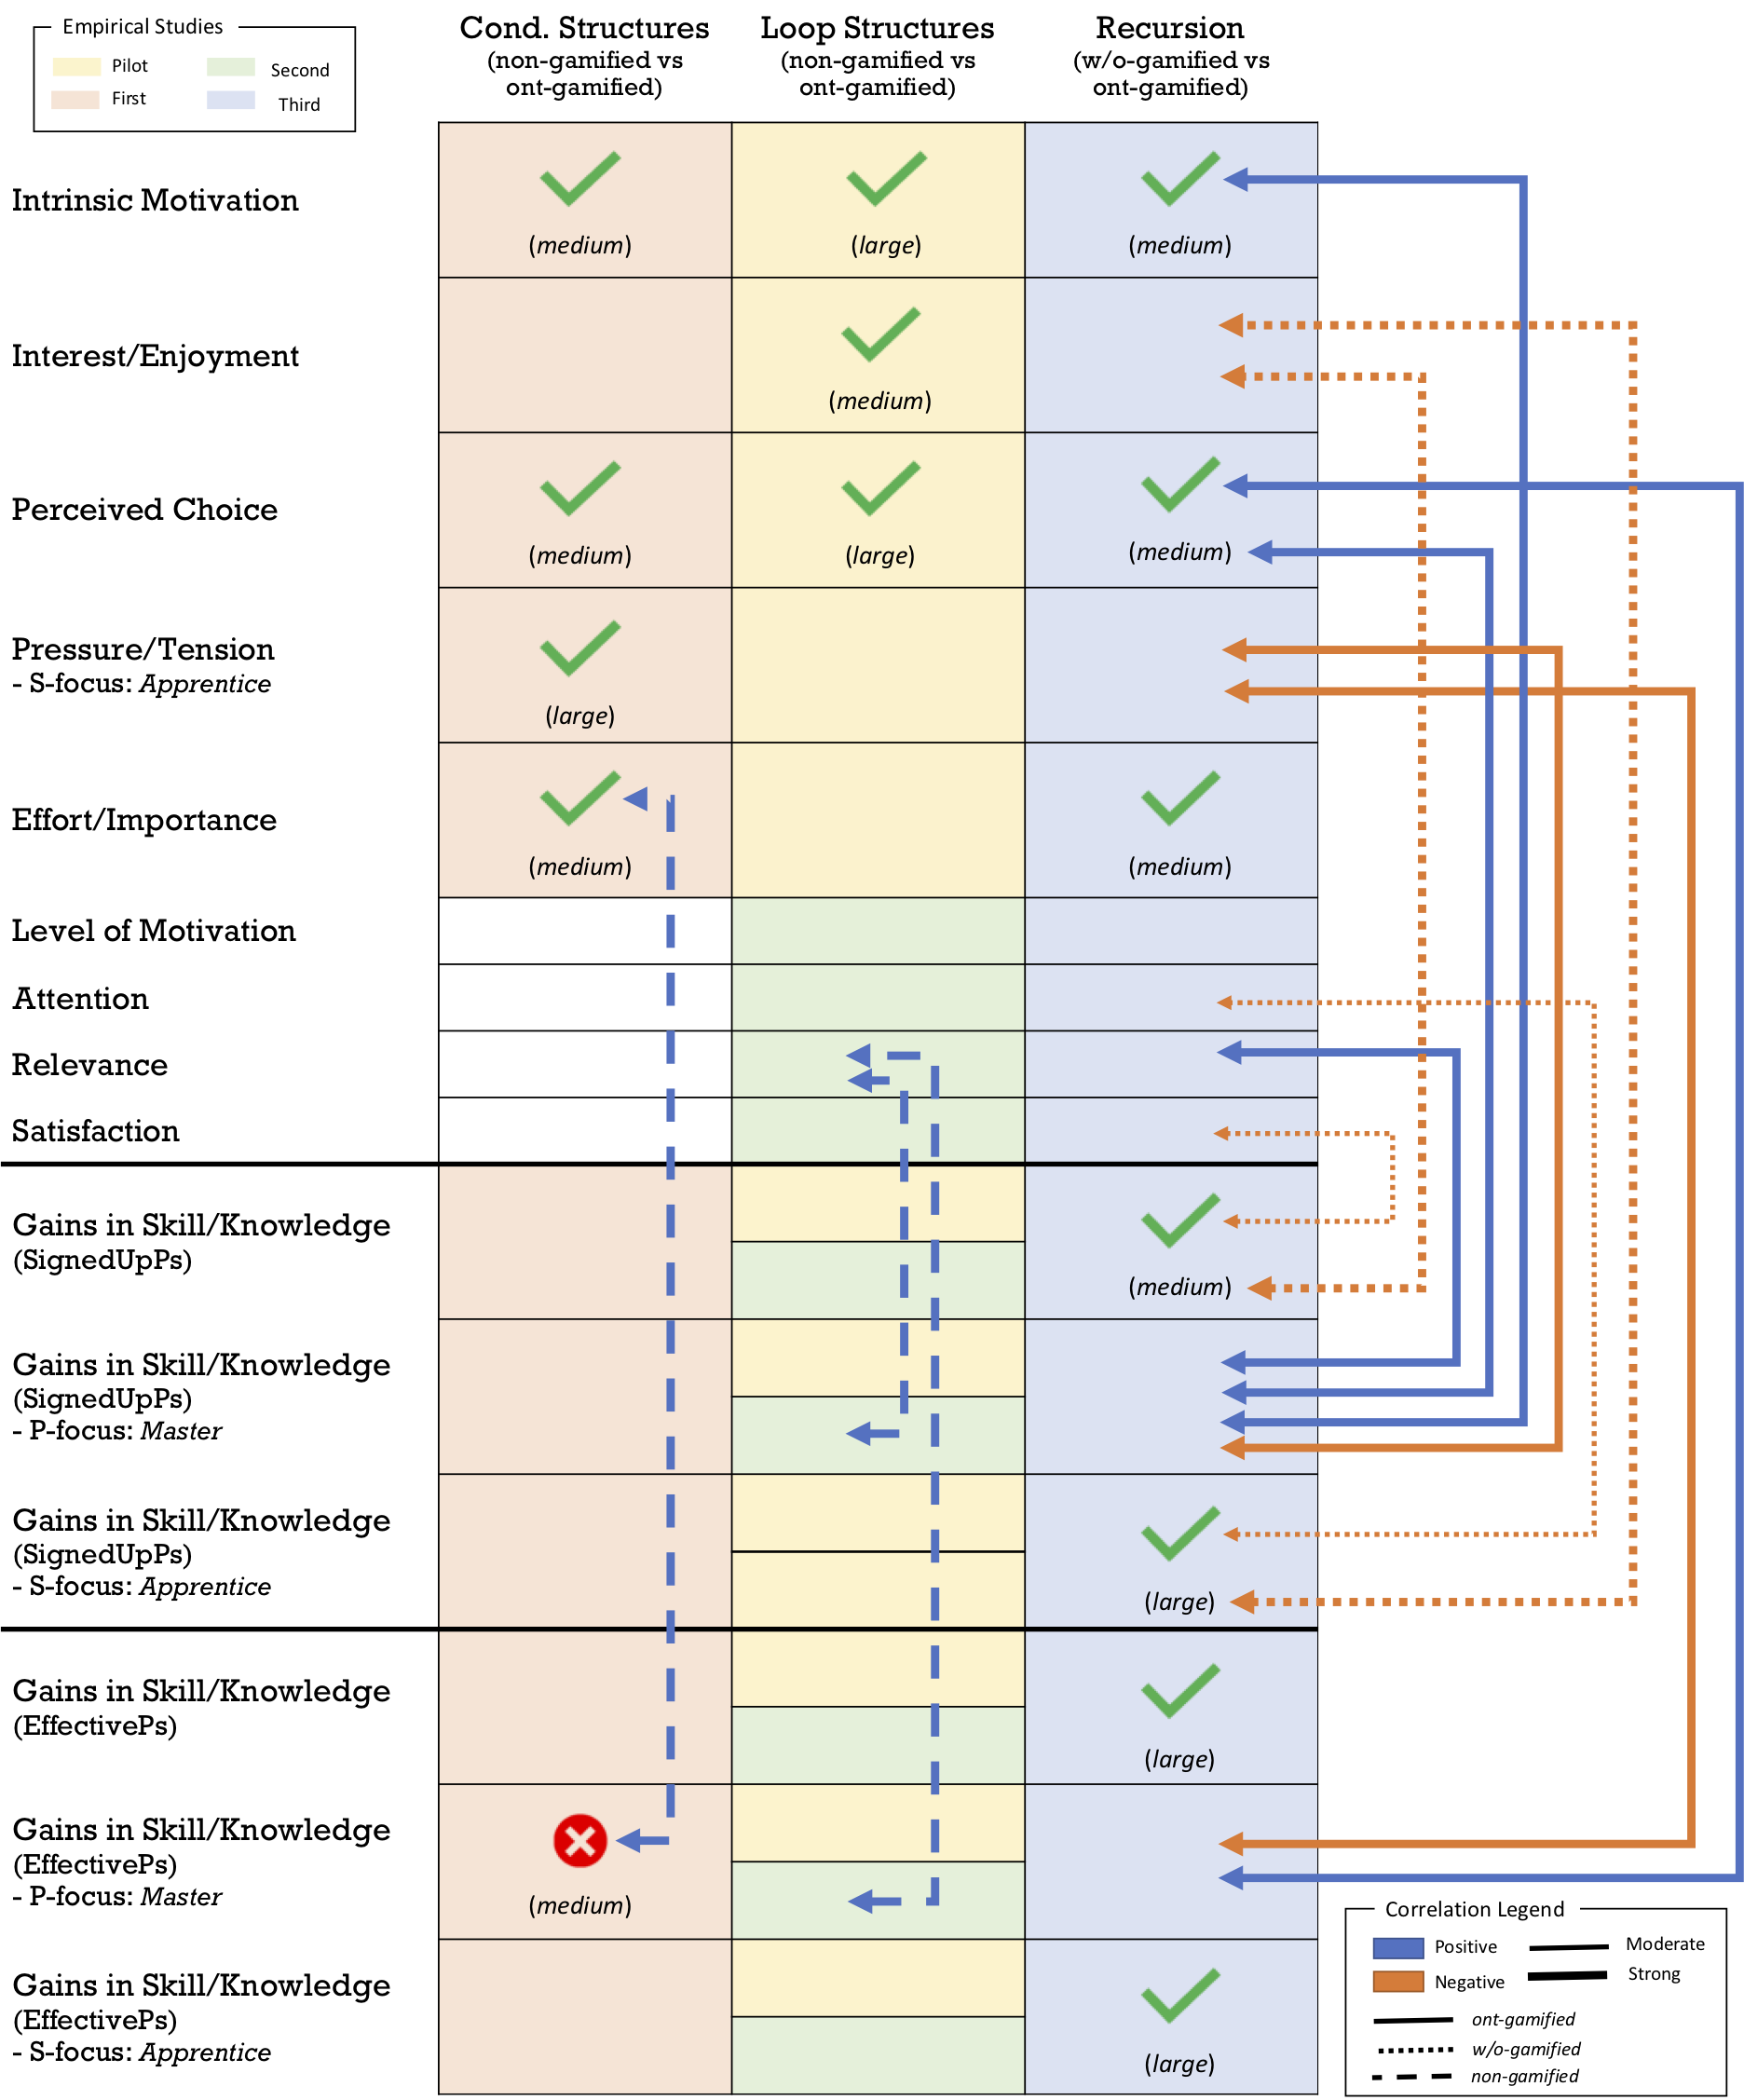
\includegraphics[width=1\textwidth]{images/chap-evaluation/cross-analysis.png}
 \fautor
\end{figure}

\subsubsection*{Assertion (2): The ontological engineering approach to gamify CL scenarios is an efficient method to deal with the motivation problem caused by the scripted collaboration because the participants in ont-gamified CL sessions have better perceived choice, intrinsic motivation and effort/importance than in w/o-gamified CL sessions.}

As was mentioned before, the sense of obligation caused by the lack of choice over the sequence of interactions defined by a CSCL script is avoided by increasing the participants' perceived choice, and the ont-gamified CL sessions in the third empirical study demonstrated their efficacy indicating that the participants' perceived choice  was greater in these sessions than in w/o-gamified CL sessions with a medium effect size. 
To avoid the motivation problem in an efficient way, the internalization of motivation should be better in ont-gamified CL sessions than in w/o-gamified CL sessions. In this sense, this efficacy has been demonstrated in the third empirical study in which the participants were significantly more intrinsic motivated in ont-gamified CL session that in w/o-gamified CL session with a medium effect size because the internalization of motivation requires that the participant to be intrinsic motivated.

\subsubsection*{Assertion (3): The ontological engineering approach to gamify CL scenarios is a method that, to obtain positive learning outcomes, affects in a proper way the participants' motivation towards CL sessions instantiated from CSCL scripts because the participants' gains in skill/knowledge as measurement of learning outcomes were not significantly different in non-gamified CL sessions and ont-gamified CL sessions, and the participants' gains in skill/knowledge obtained in ont-gamified CL sessions are better than in w/o-gamified CL sessions}

As the ontological engineering approach to gamify CL scenarios introduces extrinsic motivators in the learning environment in which the CL sessions are executed, and the extrinsic motivators have been shown to negatively affect people motivation \cite{BenabouTirole2003, FreyJegen1999}, it is likely that game elements would undermine the participants motivation' towards their participation in CL sessions instantiated from CSCL scripts, which in turn can cause unintended negative learning outcomes. In this direction, the pilot and second empirical studies demonstrated that there were not significant difference between the gains in skill/knowledge obtained by students who participated in ont-gamified CL sessions and those gains obtained by students who participated in non-gamified CL sessions.

Although, in the first empirical study, the gains in skill/knowledge obtained by the master students with effective participation in non-gamified CL sessions were significantly better than the gains in skill/knowledge obtained in ont-gamified CL sessions, this difference was apparently not related to the effects on participants' motivation caused by the game elements introduced in ont-gamified CL sessions. According to the correlation tests, there was a significant strong positive correlation between the effort/importance and the gains in skill/knowledge obtained by the master students with effective participation in non-gamified CL sessions, but there was not the same significant correlation by the master students with effective participation in ont-gamified CL sessions. It means that probably the effort/importance of master students in ont-gamified was not enough to be significant, and thus, to increase their gains in skill/knowledge in ont-gamified CL sessions. However, the effort/importance of participants (master and aprentice) in ont-gamified CL sessions were significantly greater than the effort/importance of participants in non-gamified CL session. This fact can be assumed as an contradiction to the correlation between the effort/importance and the gains in skill/knowledge whereby this correlation did not indicate a causal relationship. Furthermore, taking into account that the difficulty level of the topic (Cond. Structures) used as content-domain in the first empirical study to design the CL sessions was the easiest level of difficulty, we can hypothesize that, when the content-domain to instantiate the CL sessions has a easiest difficulty level, the game elements should increase the effort/importance of participants in the primary focus of the CSCL script to obtain at least the same gains in skill/knowledge that are obtained in non-gamified CL sessions. In the first empirical study, this primary focus was master students, and to test this hypothesis is necessary to repeat the first empirical study but using other content-domain with an easiest difficulty level.

Because the gains in skill/knowledge of signed-up students and students with effective participation were significantly greater than the gains in skill/knowledge obtained in w/o-gamified CL sessions in the third empirical study, and these gains were significantly correlated with the positive effects on the participants' motivation, the ontological engineering approach to gamify CL scenarios is considered a method to obtain more positive learning outcomes than the method to gamify CL scenarios without the support given by the ontology OntoGaCLeS. In ont-gamified CL session, by increasing the perceived choice of master students, their gains in skill/knowledge will be likely increased due to the strong positive correlation between the perceived choice and the gains in skill/knowledge obtained by signed-up master students and master students with effective participation, and due to the fact that the participants' perceived choice were significantly greater in ont-gamified CL sessions than in w/o-gamified CL sessions with a medium effect size. In ont-gamified CL sessions, the gains in skill/knowledge of signed-up master students were also significantly strong positive correlated to the intrinsic motivation, but not for the master students with effective participation, so that the gains in skill/knowledge of master students when they were influenced by an increasing in their intrinsic motivation probably occurred as consequence of interacting at least one time in the CL process with other group members.

\subsubsection*{Assertion (4): The ontological engineering approach to gamify CL sessions is a method to improve the participation in CL sessions instantiated from CSCL scripts}

The pilot empirical study demonstrated this assertion when groups of 4 to 5 members in ont-gamified CL sessions instantiated from a CSCL script based on the Cognitive Apprenticeship theory have better percentages of participations per groups than in non-gamified CL sessions. The percentage of participants per group having any participation (incomplete, semi-complete and complete participation levels  for the signed-up students) were significantly greater in ont-gamified CL sessions than in non-gamified CL sessions, and the percentages of participants per group having an incomplete participation (none and incomplete participation levels for the signed-up students) and without participation (none participation level for the signed-up students) were significantly less in ont-gamified CL sessions than in non-gamified CL sessions.

